\subsection{Thiết kế giao diện}
% --- NHÓM 1: XÁC THỰC (AUTHENTICATION) ---

\begin{figure}[H]
    \centering
    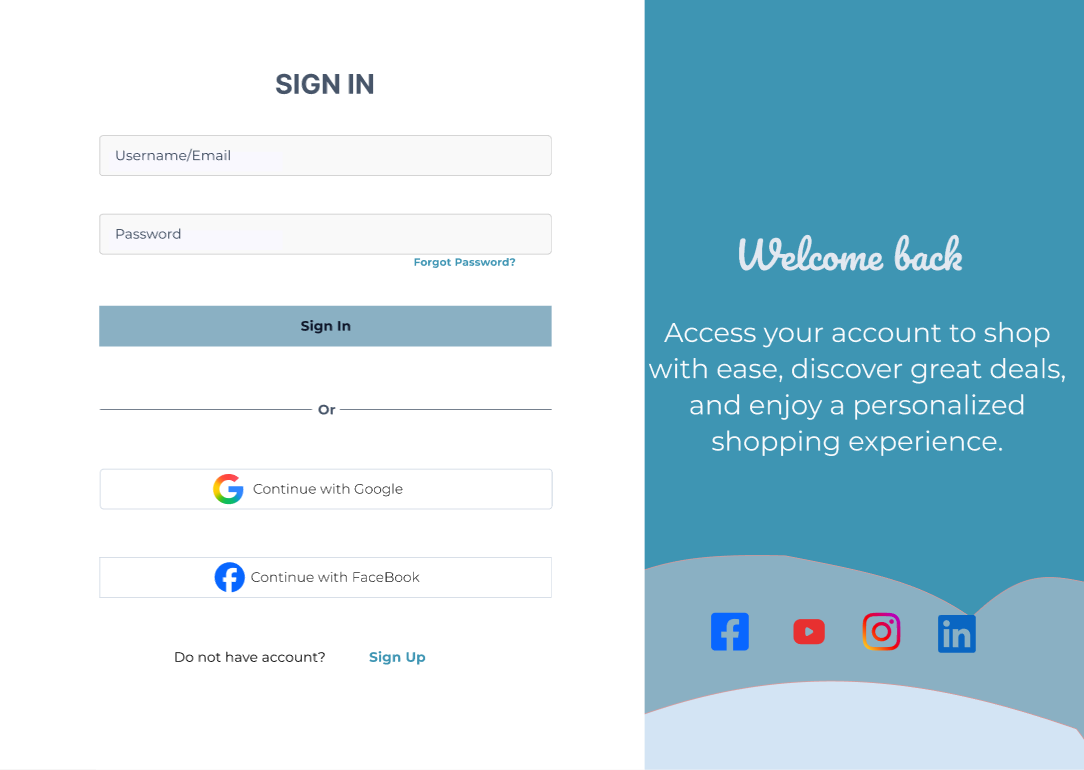
\includegraphics[width=0.8\linewidth]{images/ui/ui_login.png}
   \vspace{0.5cm} \caption{Giao diện Đăng nhập}
    \label{fig:ui_login}
\end{figure}
Giao diện đăng nhập được thiết kế tối giản, tập trung vào form điền thông tin (Email/Tên đăng nhập và Mật khẩu). Hỗ trợ các tính năng tiện ích như "Ghi nhớ đăng nhập" và liên kết nhanh đến trang "Quên mật khẩu" hoặc "Đăng ký" cho người dùng mới.

\begin{figure}[H]
    \centering
    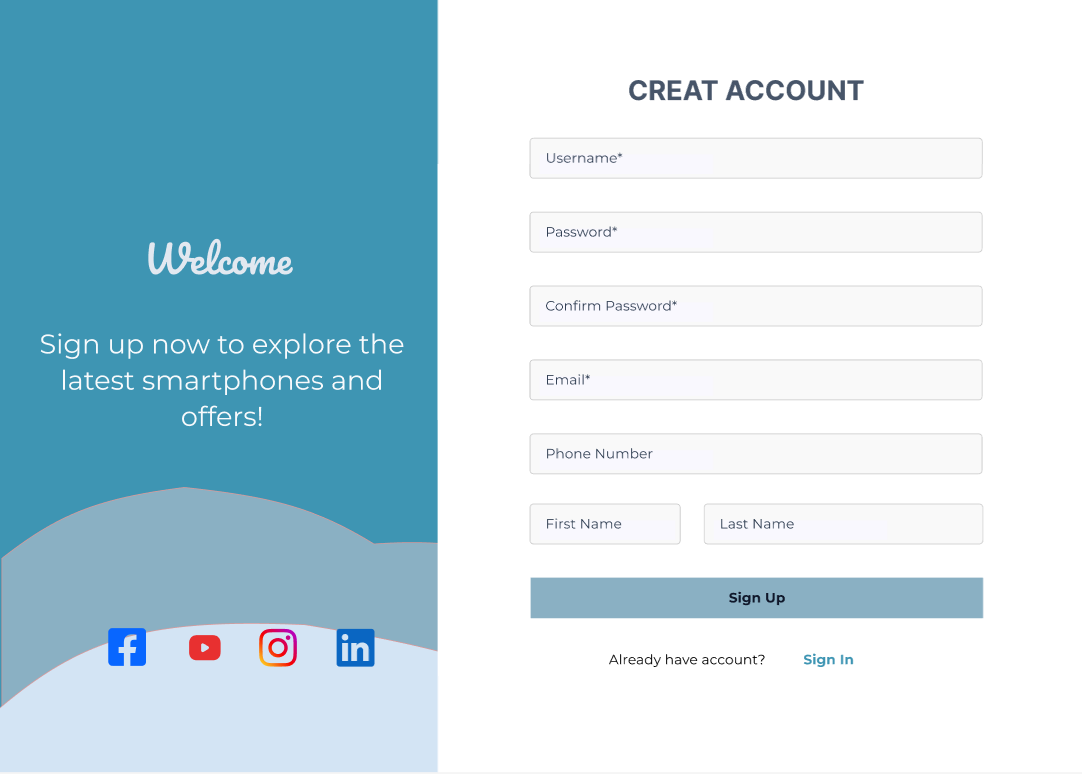
\includegraphics[width=0.8\linewidth]{images/ui/ui_register.png}
   \vspace{0.5cm} \caption{Giao diện Đăng ký tài khoản}
    \label{fig:ui_register}
\end{figure}
Form đăng ký yêu cầu người dùng cung cấp các thông tin thiết yếu để khởi tạo hồ sơ khách hàng. Hệ thống tích hợp xác thực dữ liệu (validation) theo thời gian thực để đảm bảo định dạng email và độ mạnh mật khẩu phù hợp.

\begin{figure}[H]
    \centering
    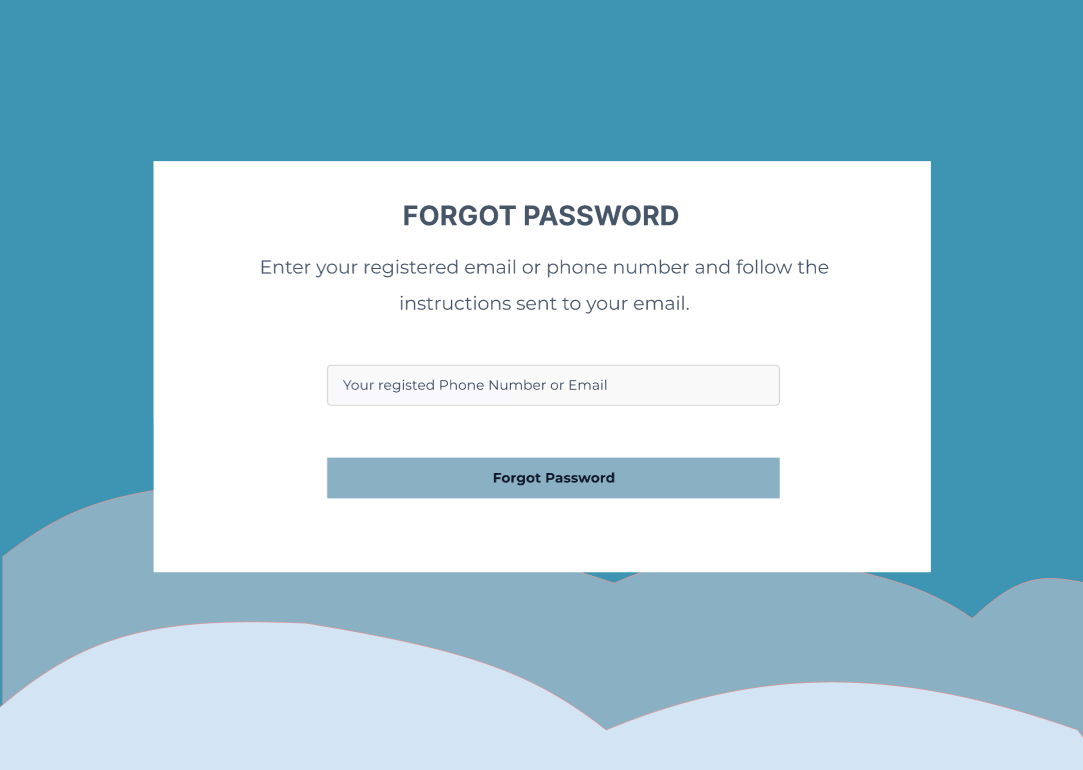
\includegraphics[width=0.8\linewidth]{images/ui/ui_forgot_password.png}
   \vspace{0.5cm} \caption{Giao diện Quên mật khẩu}
    \label{fig:ui_forgot_pass}
\end{figure}
Quy trình khôi phục tài khoản bắt đầu bằng việc người dùng nhập email đã đăng ký. Giao diện hướng dẫn rõ ràng các bước tiếp theo để nhận mã xác thực hoặc đường dẫn đặt lại mật khẩu.

\begin{figure}[H]
    \centering
    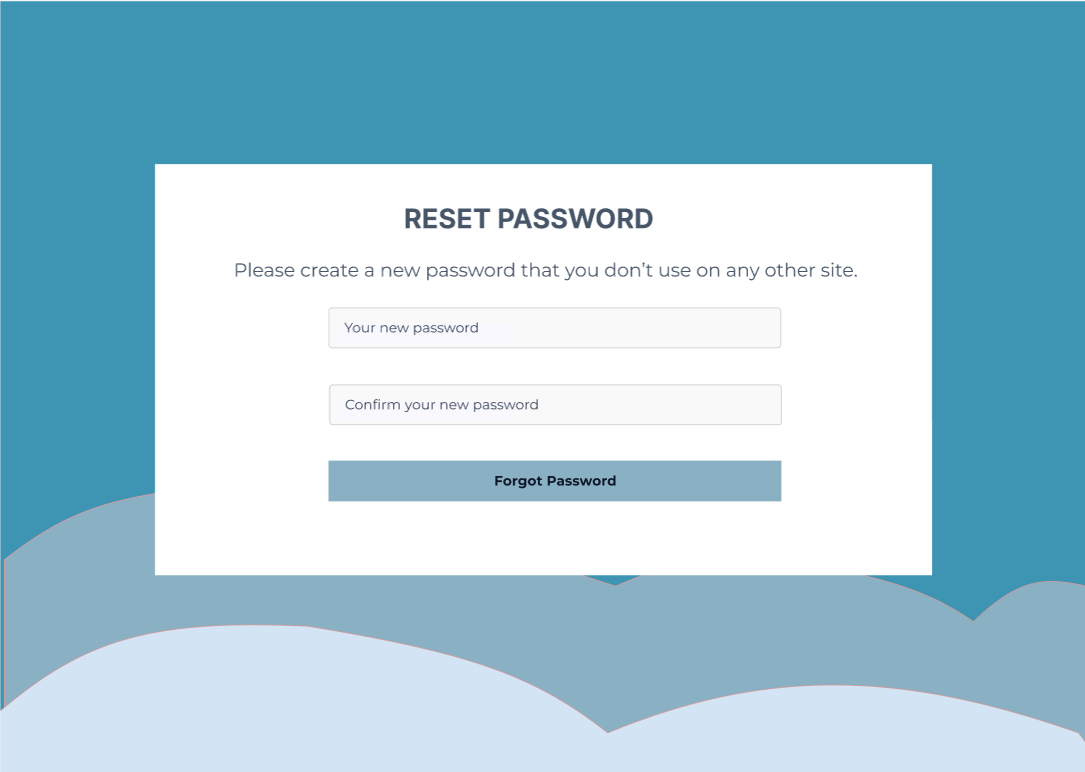
\includegraphics[width=0.8\linewidth]{images/ui/ui_reset_password.png}
   \vspace{0.5cm} \caption{Giao diện Đặt lại mật khẩu}
    \label{fig:ui_reset_pass}
\end{figure}
Sau khi xác thực thành công, người dùng được chuyển đến giao diện này để thiết lập mật khẩu mới.

% --- NHÓM 2: TRANG CHỦ & ĐIỀU HƯỚNG (BROWSING) ---

\begin{figure}[H]
    \centering
    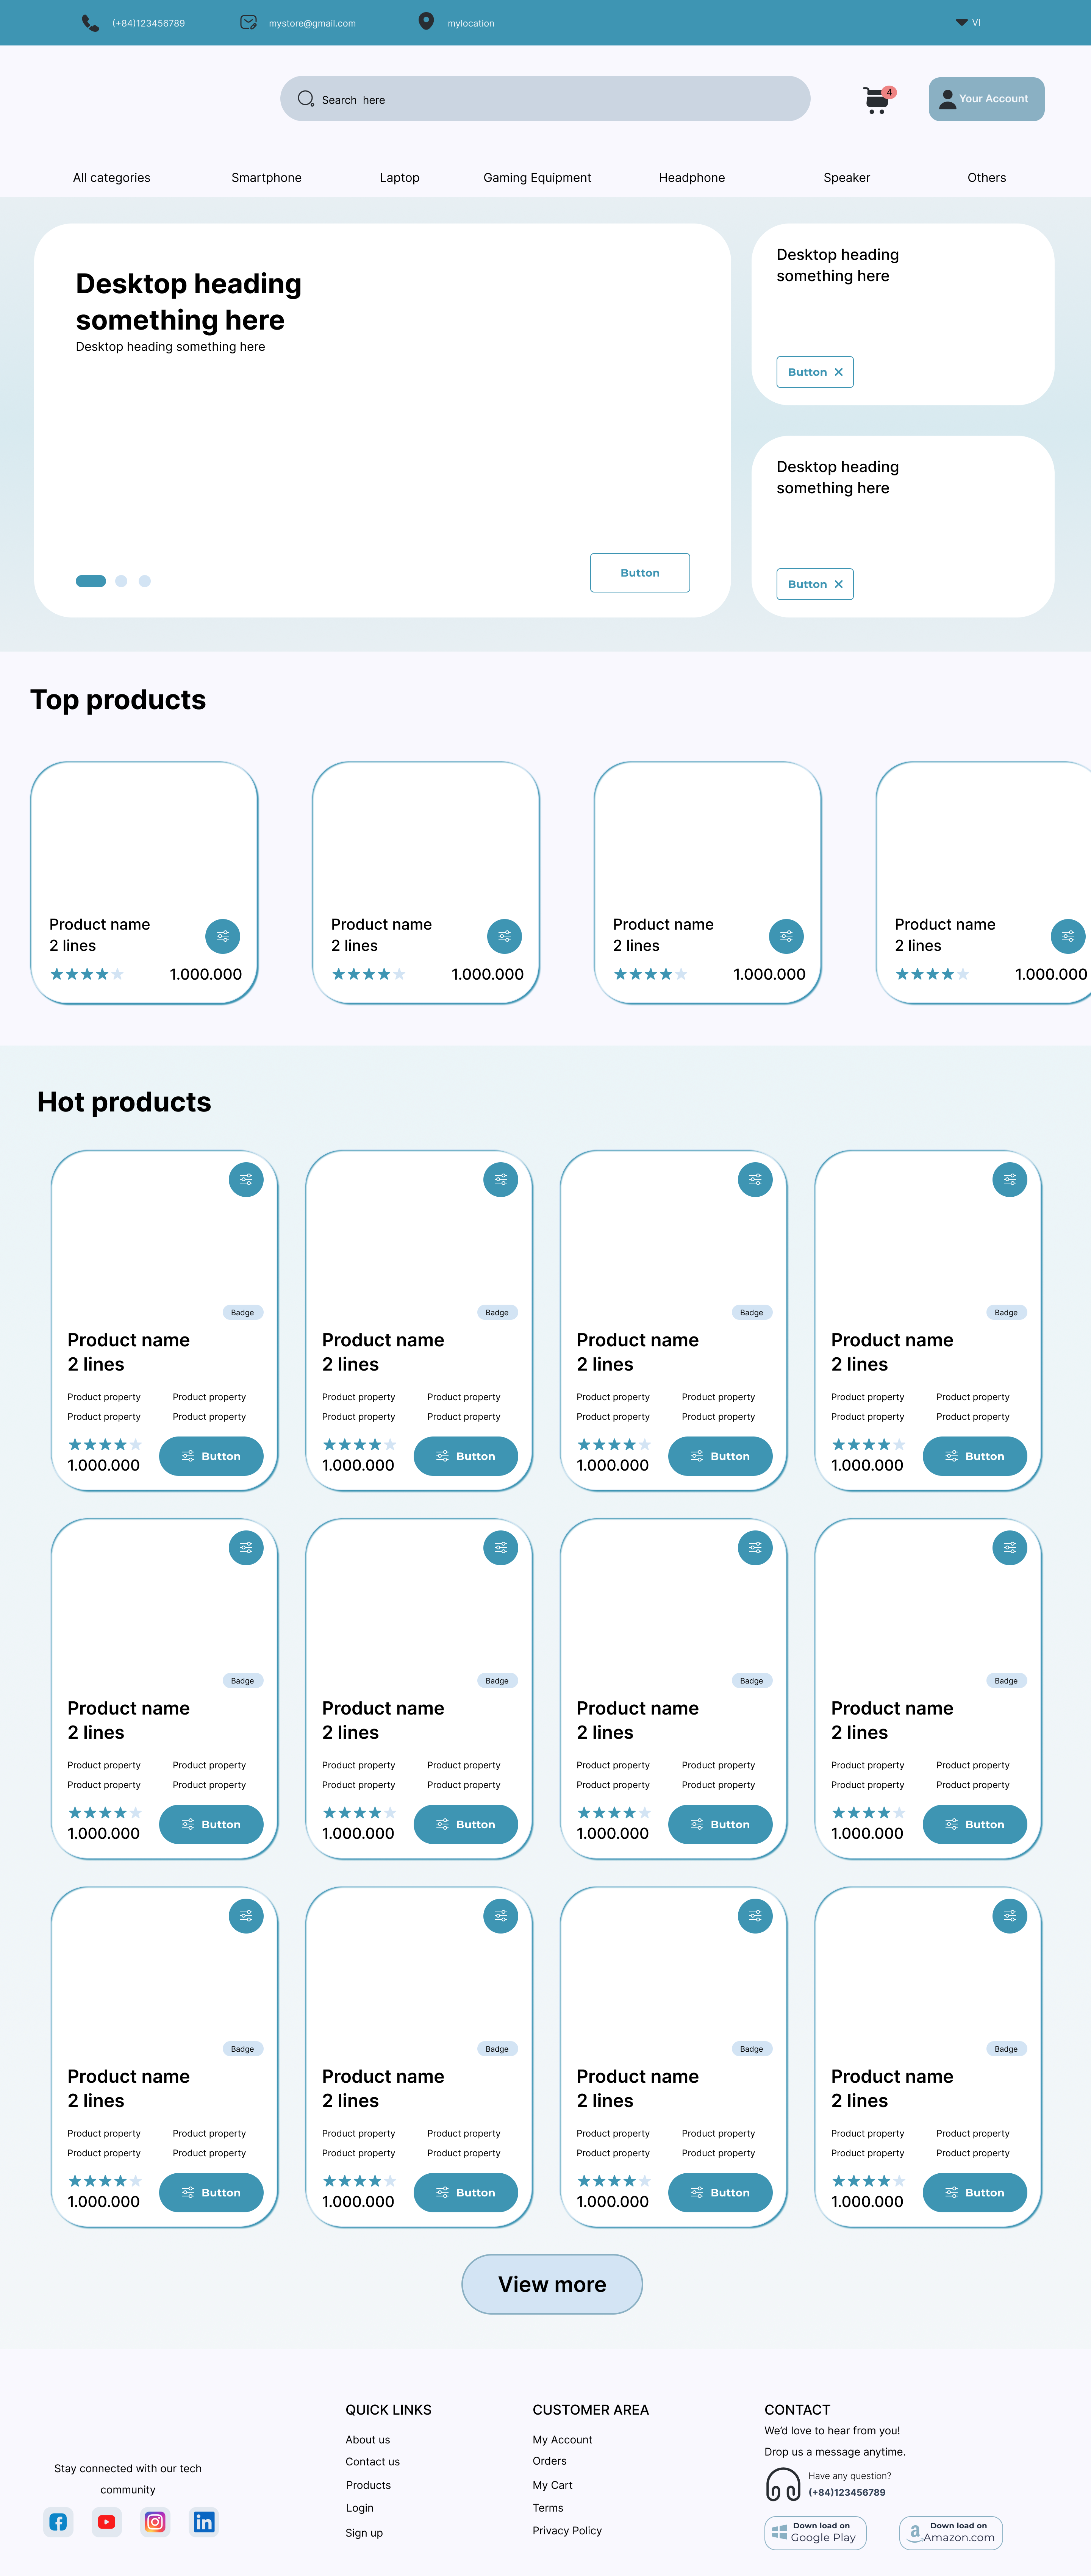
\includegraphics[width=0.6\linewidth]{images/ui/ui_home.png}
   \vspace{0.5cm} \caption{Giao diện Trang chủ (Home Page)}
    \label{fig:ui_home}
\end{figure}
Trang chủ là trung tâm điều hướng, hiển thị các Banner khuyến mãi lớn để thu hút sự chú ý.  Các danh mục sản phẩm công nghệ (Laptop, Điện thoại, Phụ kiện) được phân chia rõ ràng, kèm theo các phần "Sản phẩm bán chạy" hoặc "Hàng mới về" để kích thích nhu cầu mua sắm.

\begin{figure}[H]
    \centering
    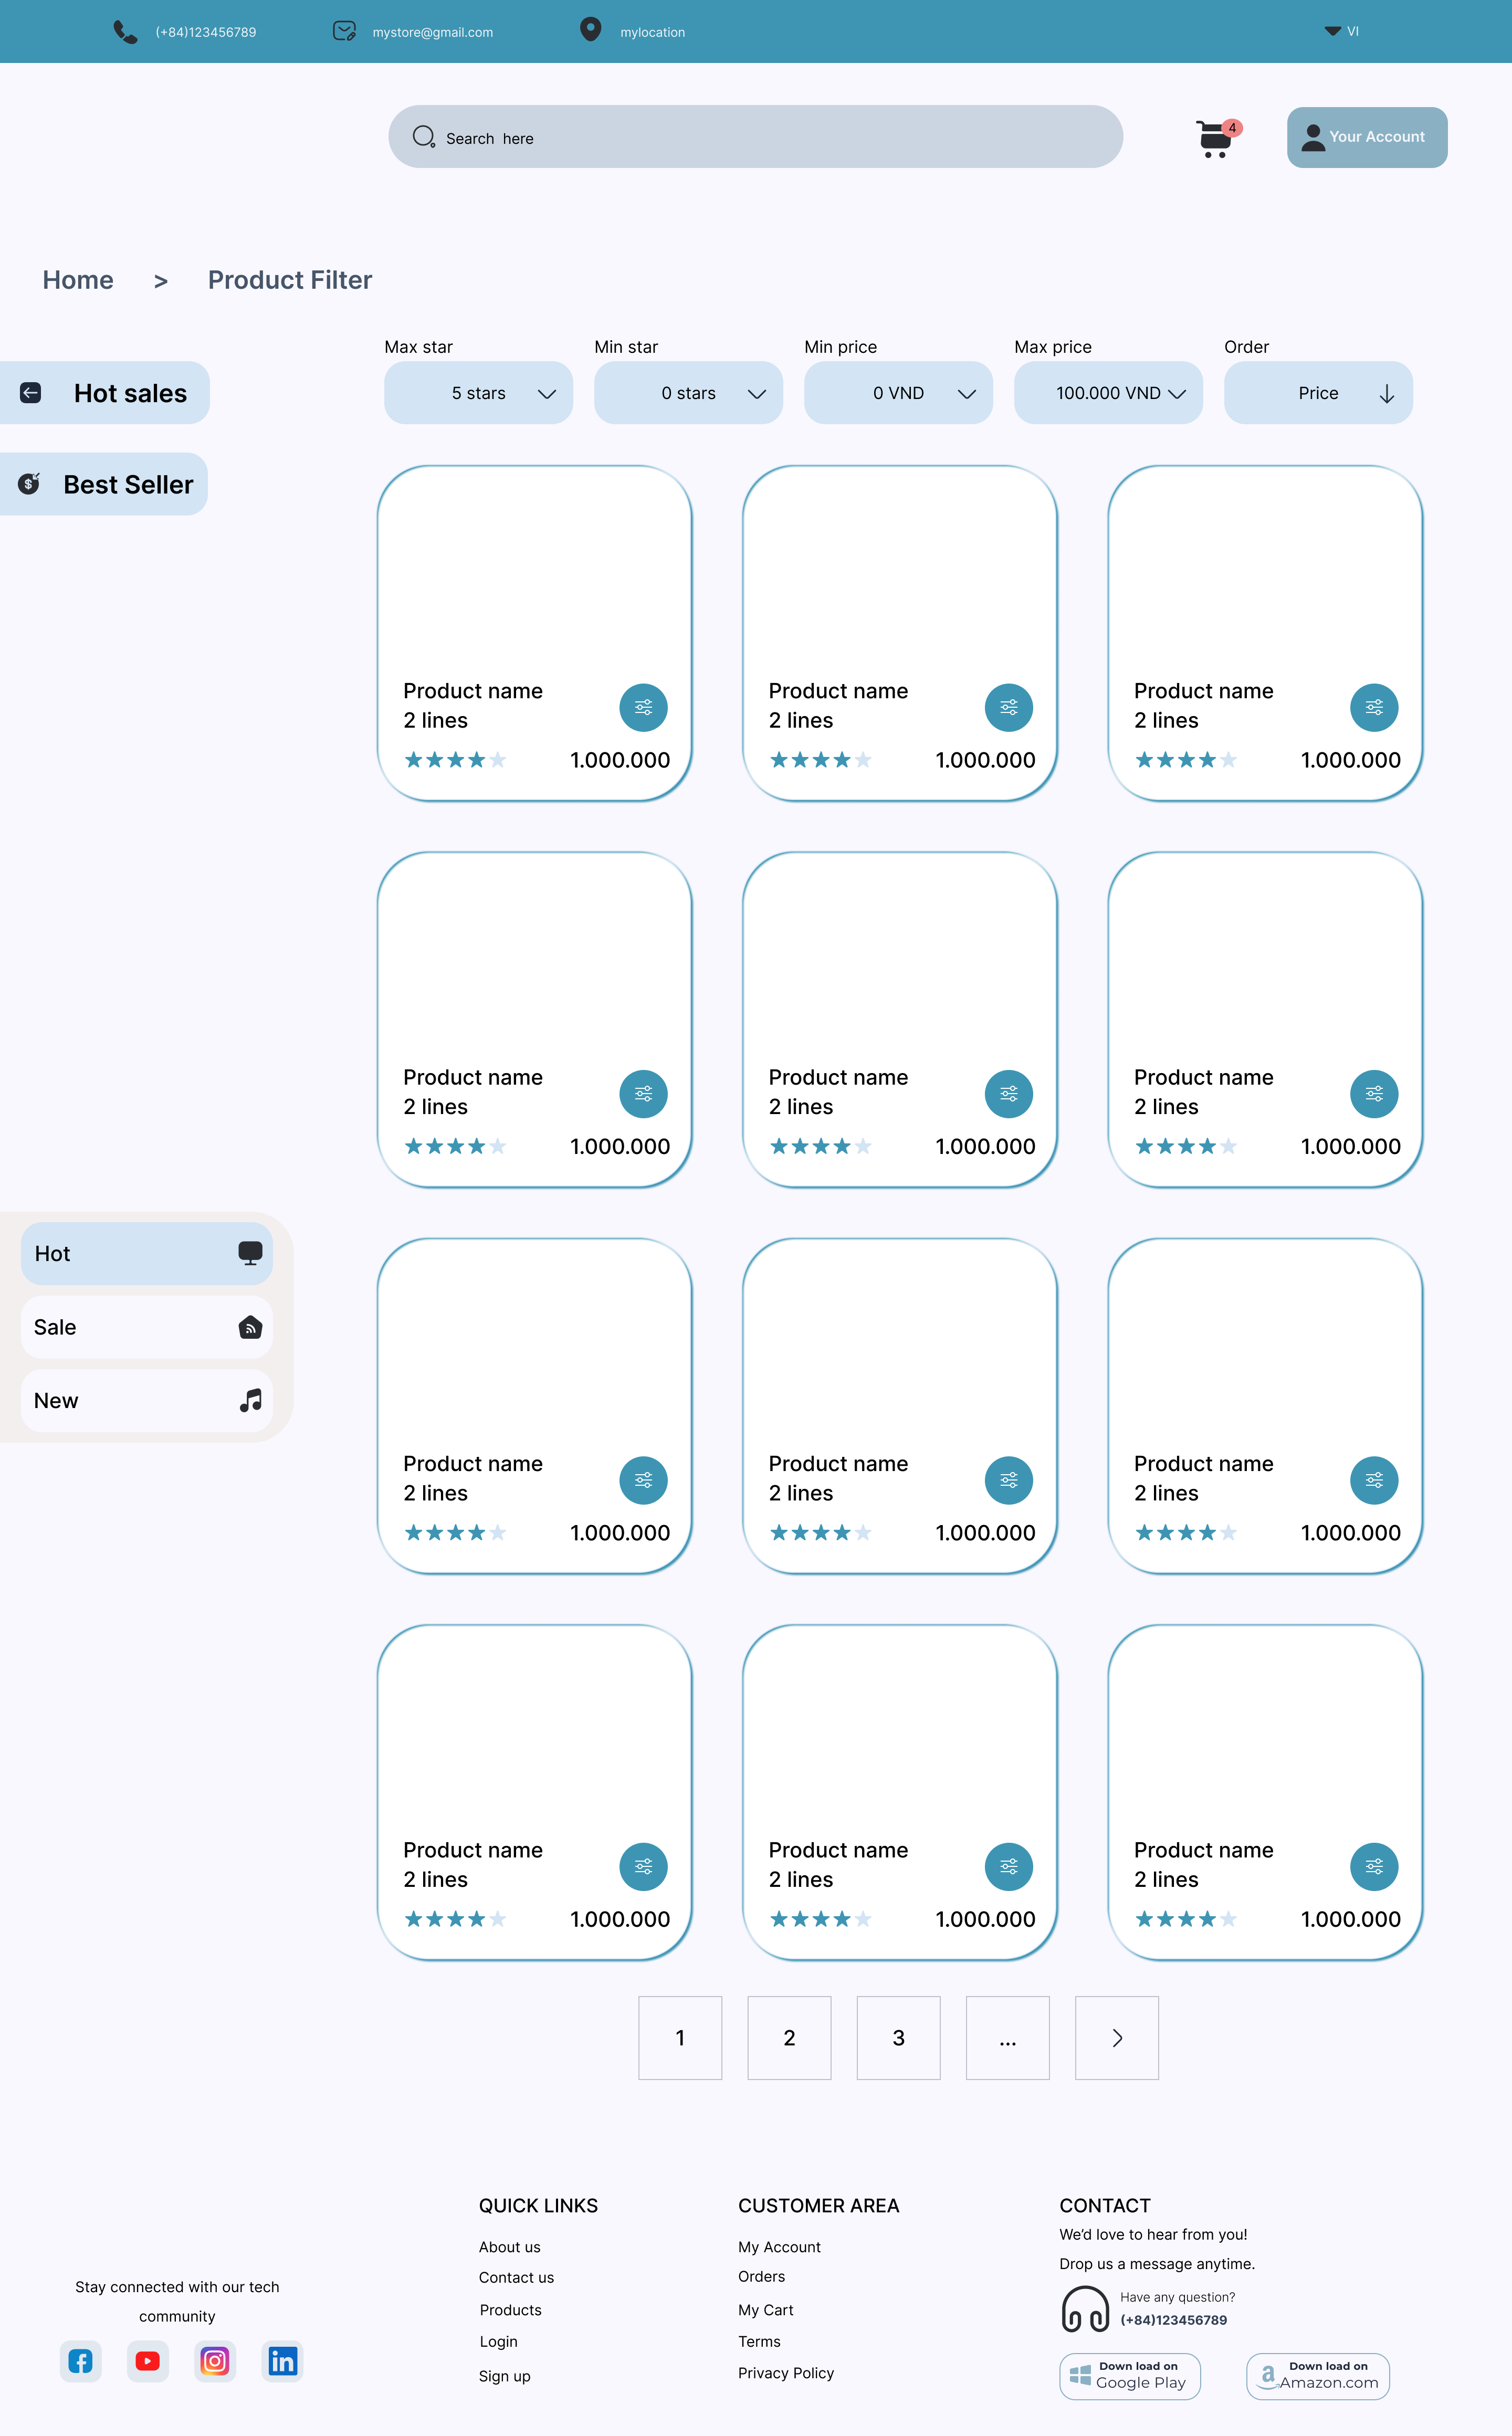
\includegraphics[width=0.8\linewidth]{images/ui/ui_about_us.png}
   \vspace{0.5cm} \caption{Giao diện Giới thiệu (About Us)}
    \label{fig:ui_about}
\end{figure}
Trang cung cấp thông tin về doanh nghiệp, sứ mệnh và cam kết chất lượng dịch vụ, giúp xây dựng lòng tin với khách hàng khi mua sắm các thiết bị điện tử giá trị cao.

\begin{figure}[H]
    \centering
    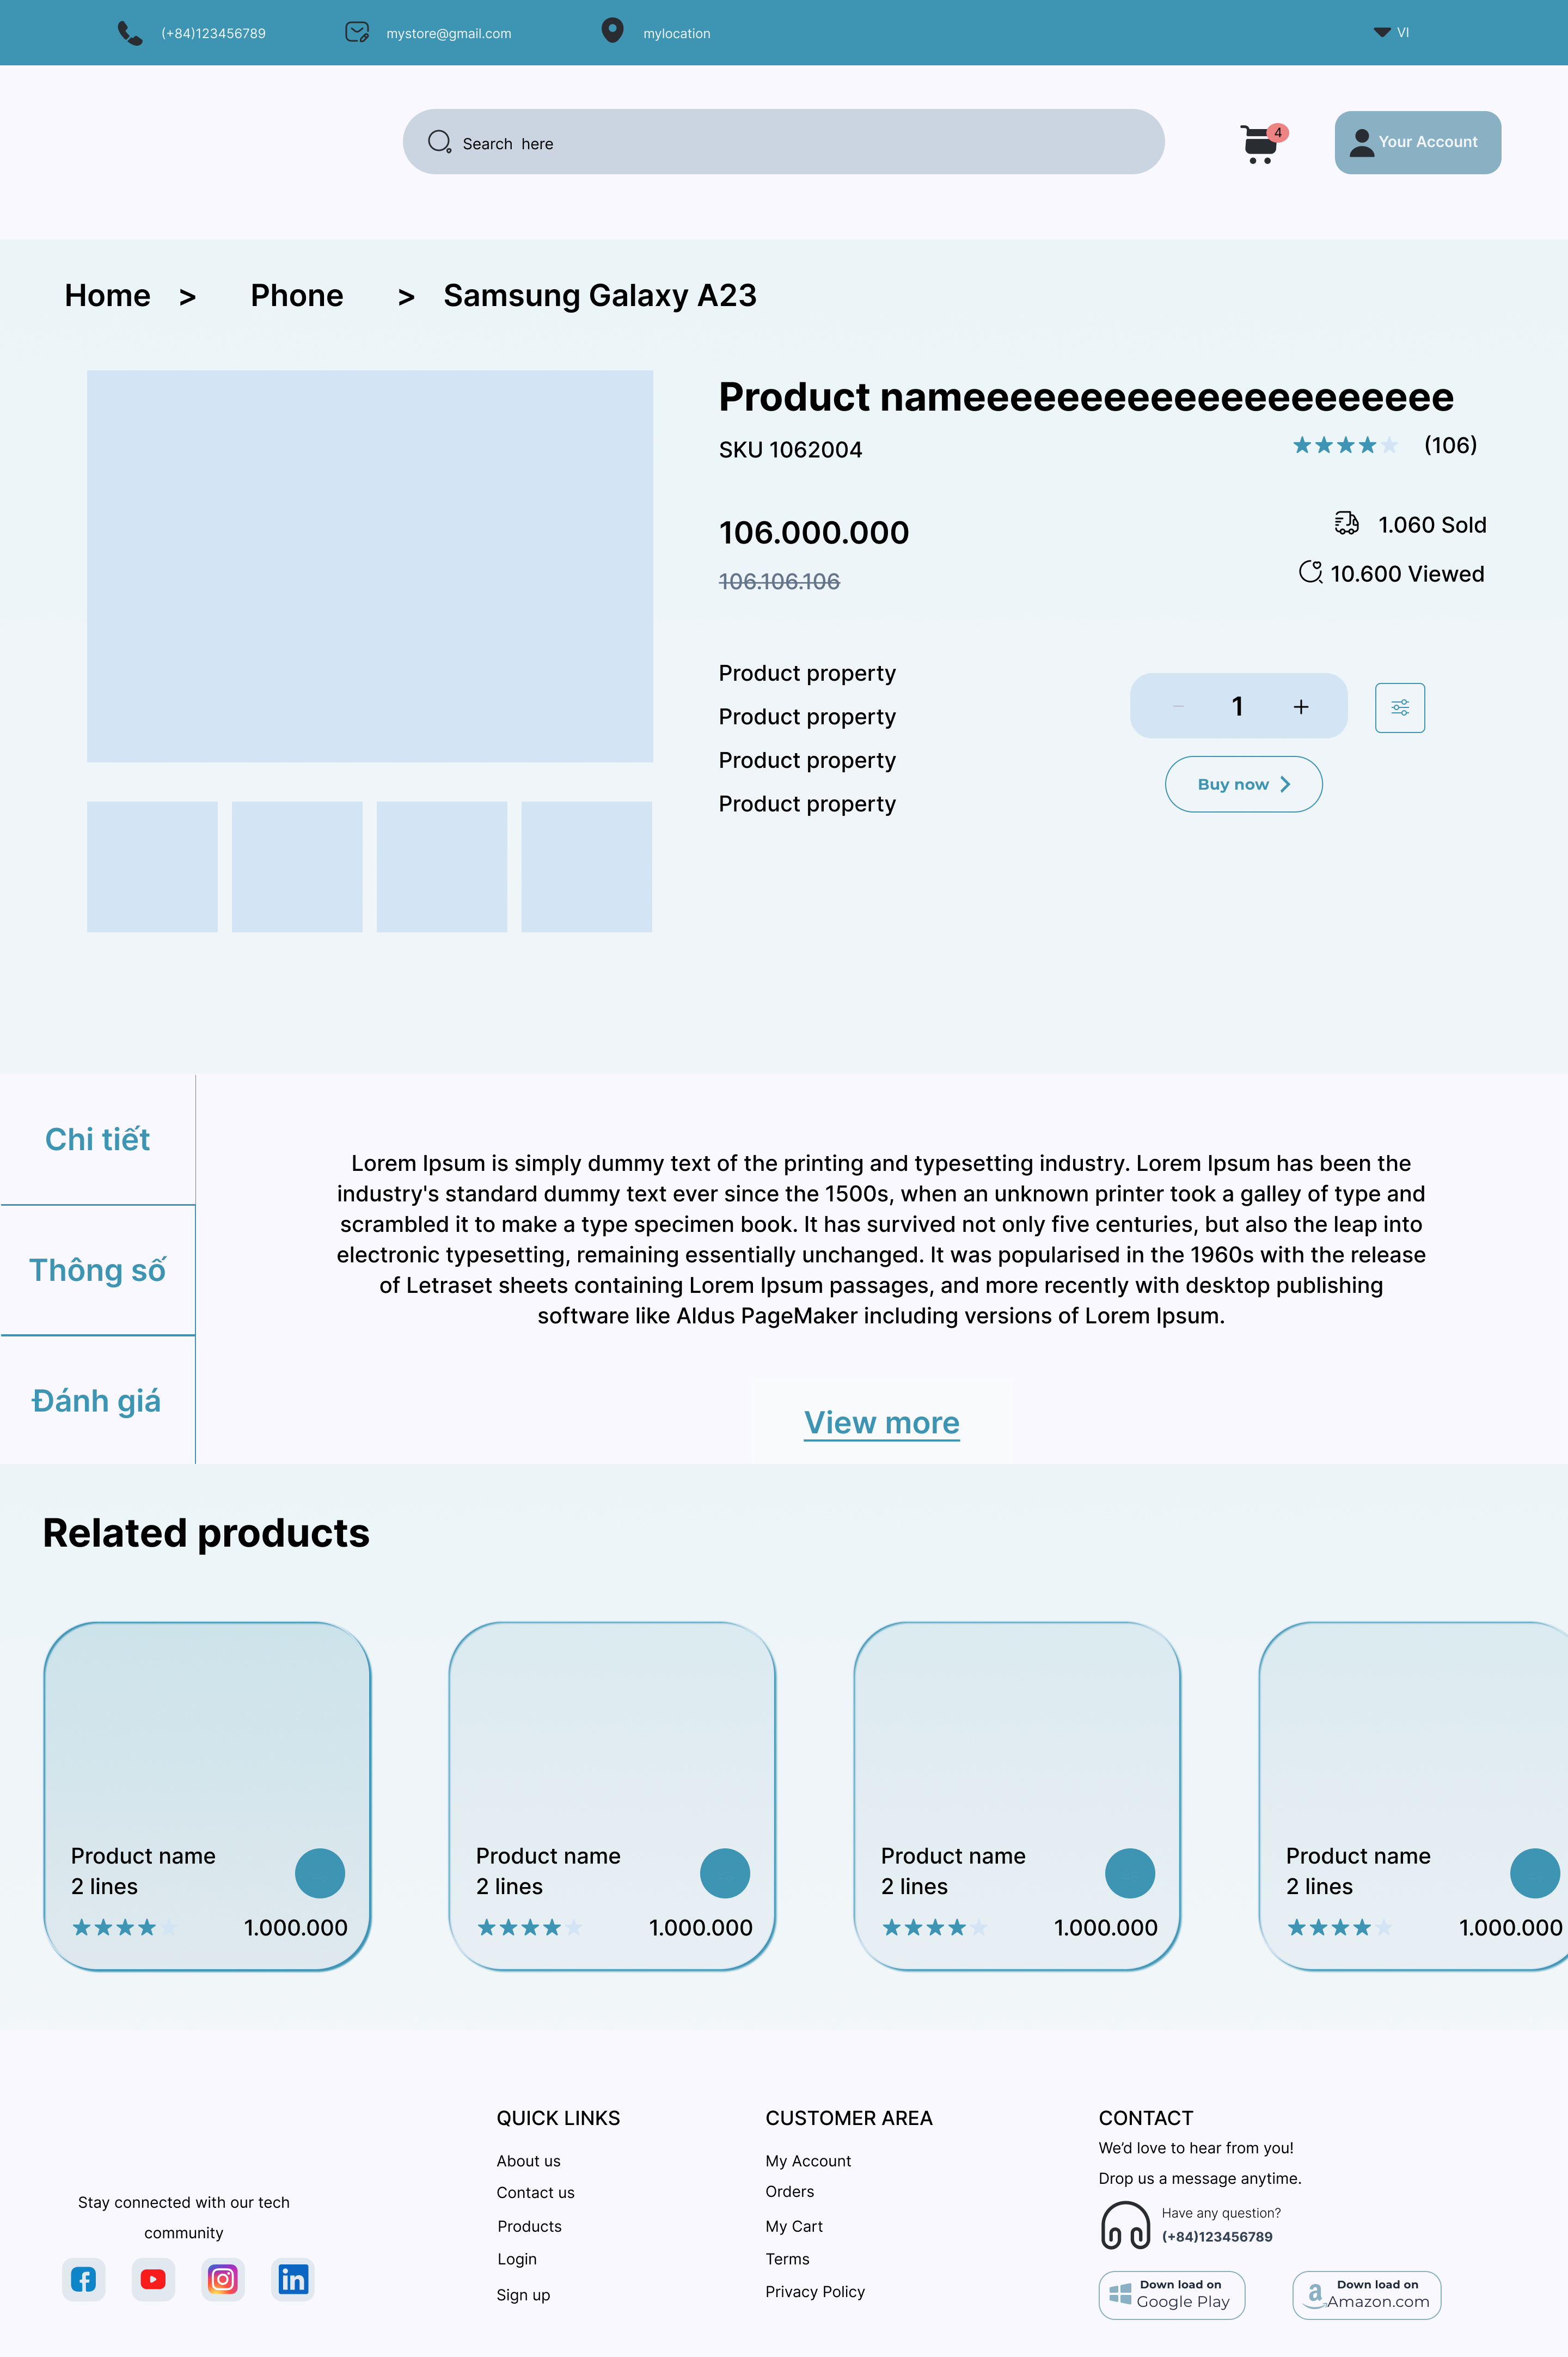
\includegraphics[width=0.9\linewidth]{images/ui/ui_product_filter.png}
   \vspace{0.5cm} \caption{Giao diện Danh sách và Bộ lọc sản phẩm}
    \label{fig:ui_filter}
\end{figure}
Giao diện danh mục sản phẩm tích hợp bộ lọc nâng cao (Sidebar Filter). Người dùng có thể lọc theo: Khoảng giá, Thương hiệu (Apple, Samsung, Dell...), Thông số kỹ thuật (RAM, SSD, Chipset) - yếu tố quan trọng nhất đối với web bán đồ công nghệ.

\begin{figure}[H]
    \centering
    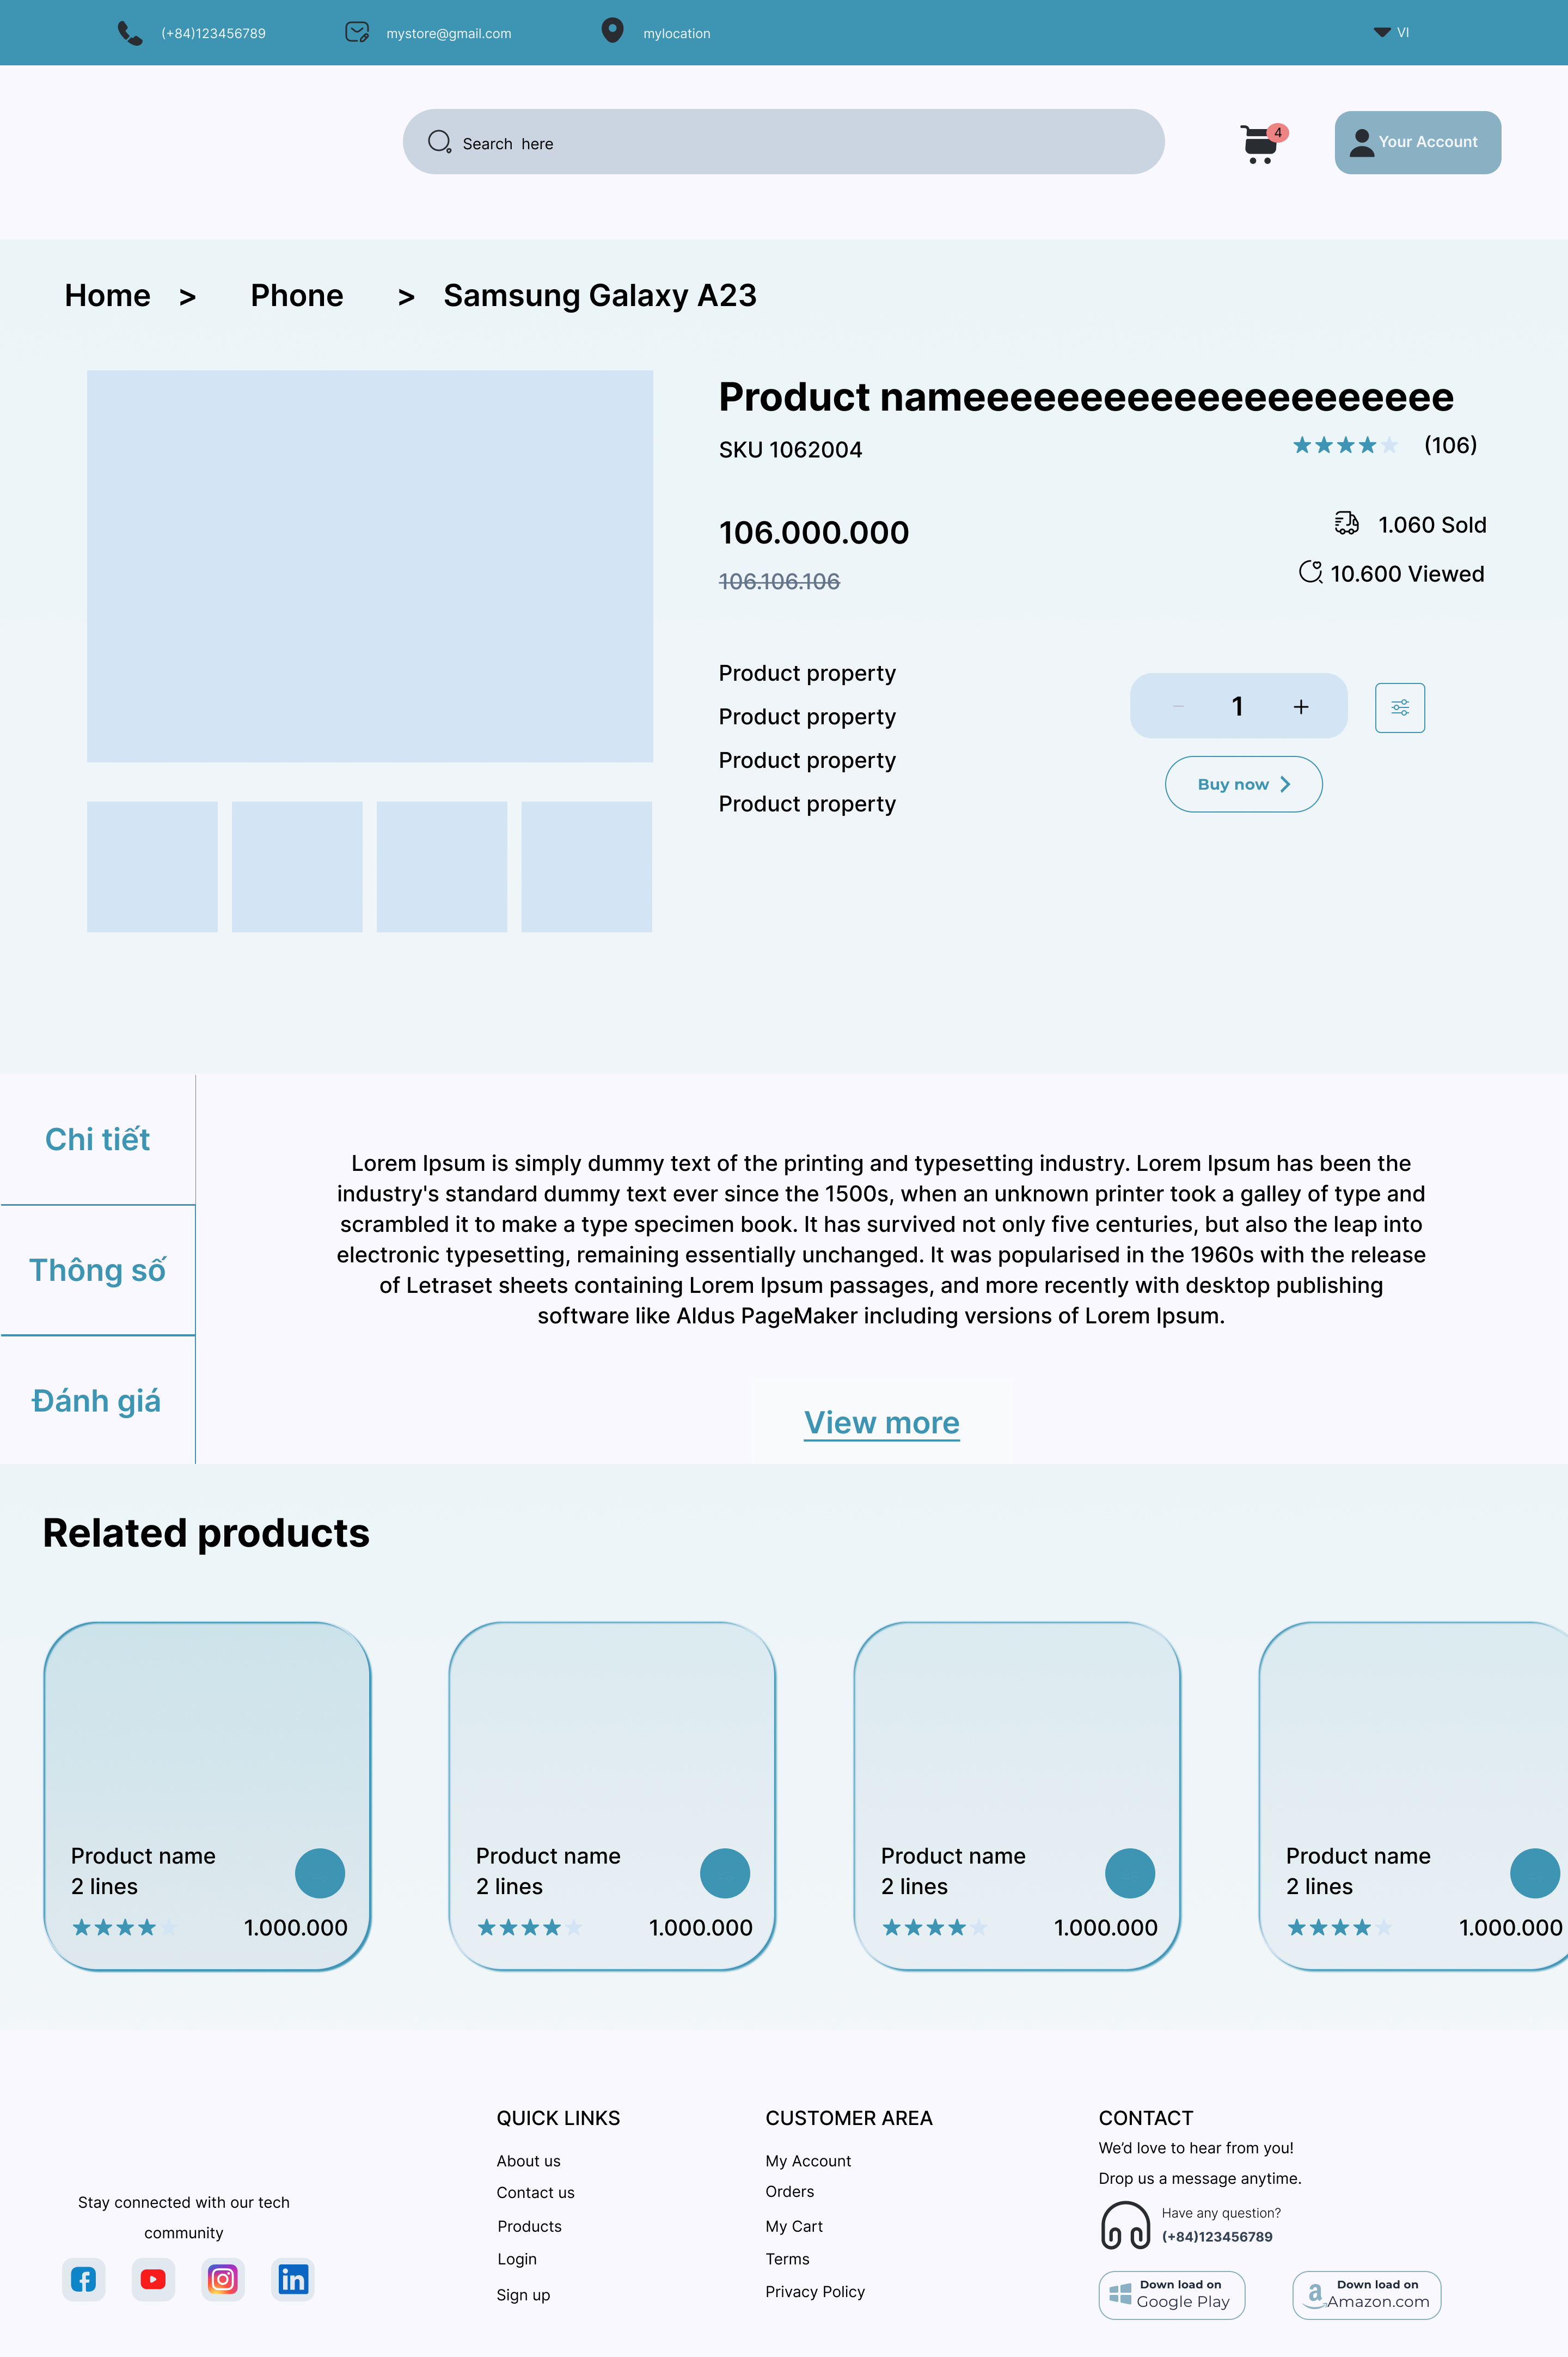
\includegraphics[width=0.9\linewidth]{images/ui/ui_profuct_detail.png}
   \vspace{0.5cm} \caption{Giao diện Chi tiết sản phẩm}
    \label{fig:ui_product_detail}
\end{figure}
Trang chi tiết cung cấp đầy đủ thông tin: Hình ảnh sản phẩm độ nét cao, thông số kỹ thuật chi tiết, tình trạng kho hàng, các tùy chọn phiên bản (Màu sắc, Cấu hình) và nút "Thêm vào giỏ hàng" (Call-to-Action) nổi bật.

\begin{figure}[H]
    \centering
    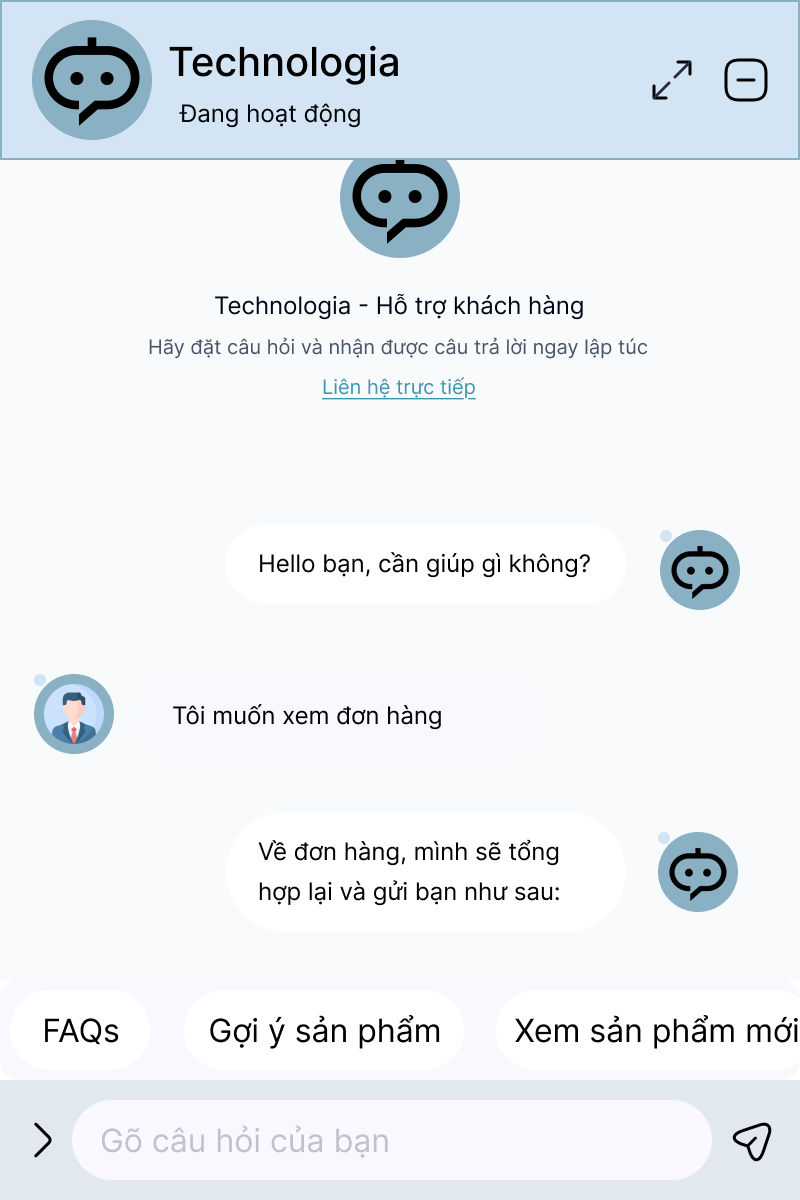
\includegraphics[width=0.4\linewidth]{images/ui/ui_chatbot.png}
   \vspace{0.5cm} \caption{Giao diện Chatbot hỗ trợ}
    \label{fig:ui_chatbot}
\end{figure}
Cửa sổ Chatbot AI tích hợp ở góc màn hình, hỗ trợ giải đáp nhanh các câu hỏi thường gặp về cấu hình máy, chính sách bảo hành hoặc hướng dẫn đặt hàng 24/7. 



% --- NHÓM 3: MUA HÀNG & THANH TOÁN (CHECKOUT) ---

\begin{figure}[H]
    \centering
    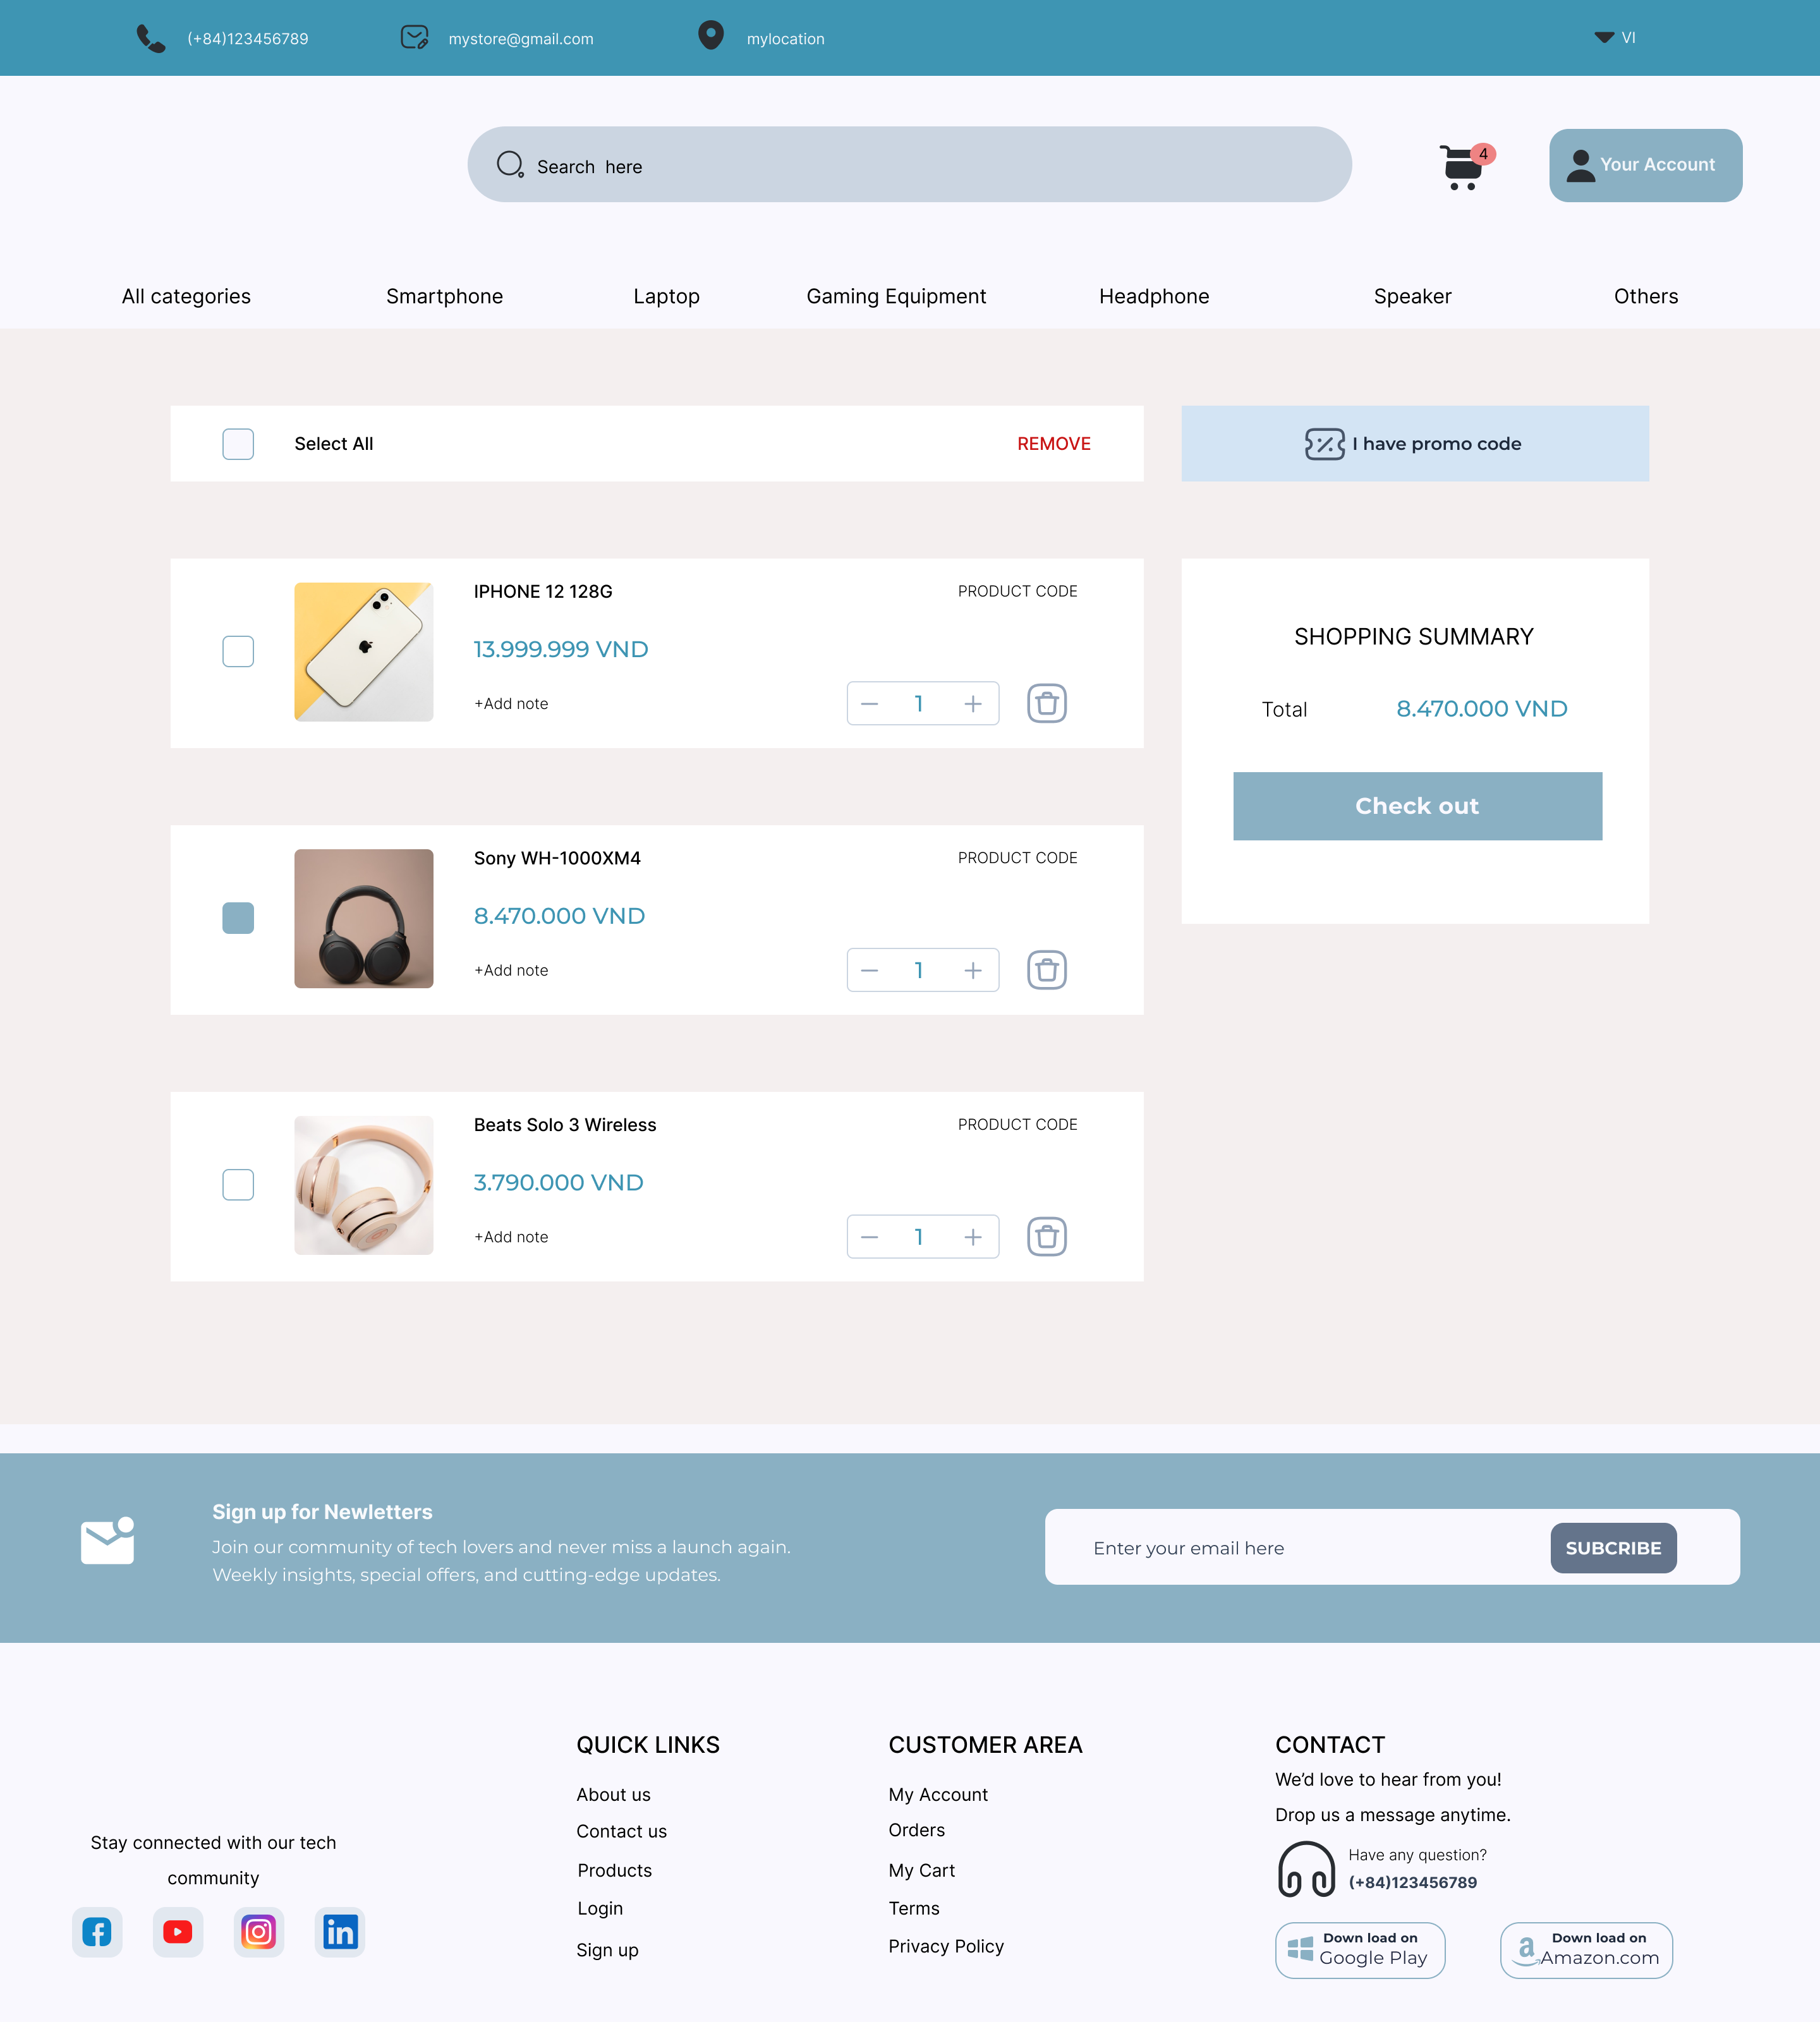
\includegraphics[width=0.9\linewidth]{images/ui/ui_cart.png}
   \vspace{0.5cm} \caption{Giao diện Giỏ hàng}
    \label{fig:ui_cart}
\end{figure}
Người dùng xem lại danh sách sản phẩm đã chọn, điều chỉnh số lượng hoặc xóa bớt sản phẩm. Tổng giá trị đơn hàng được cập nhật tự động.

\begin{figure}[H]
    \centering
    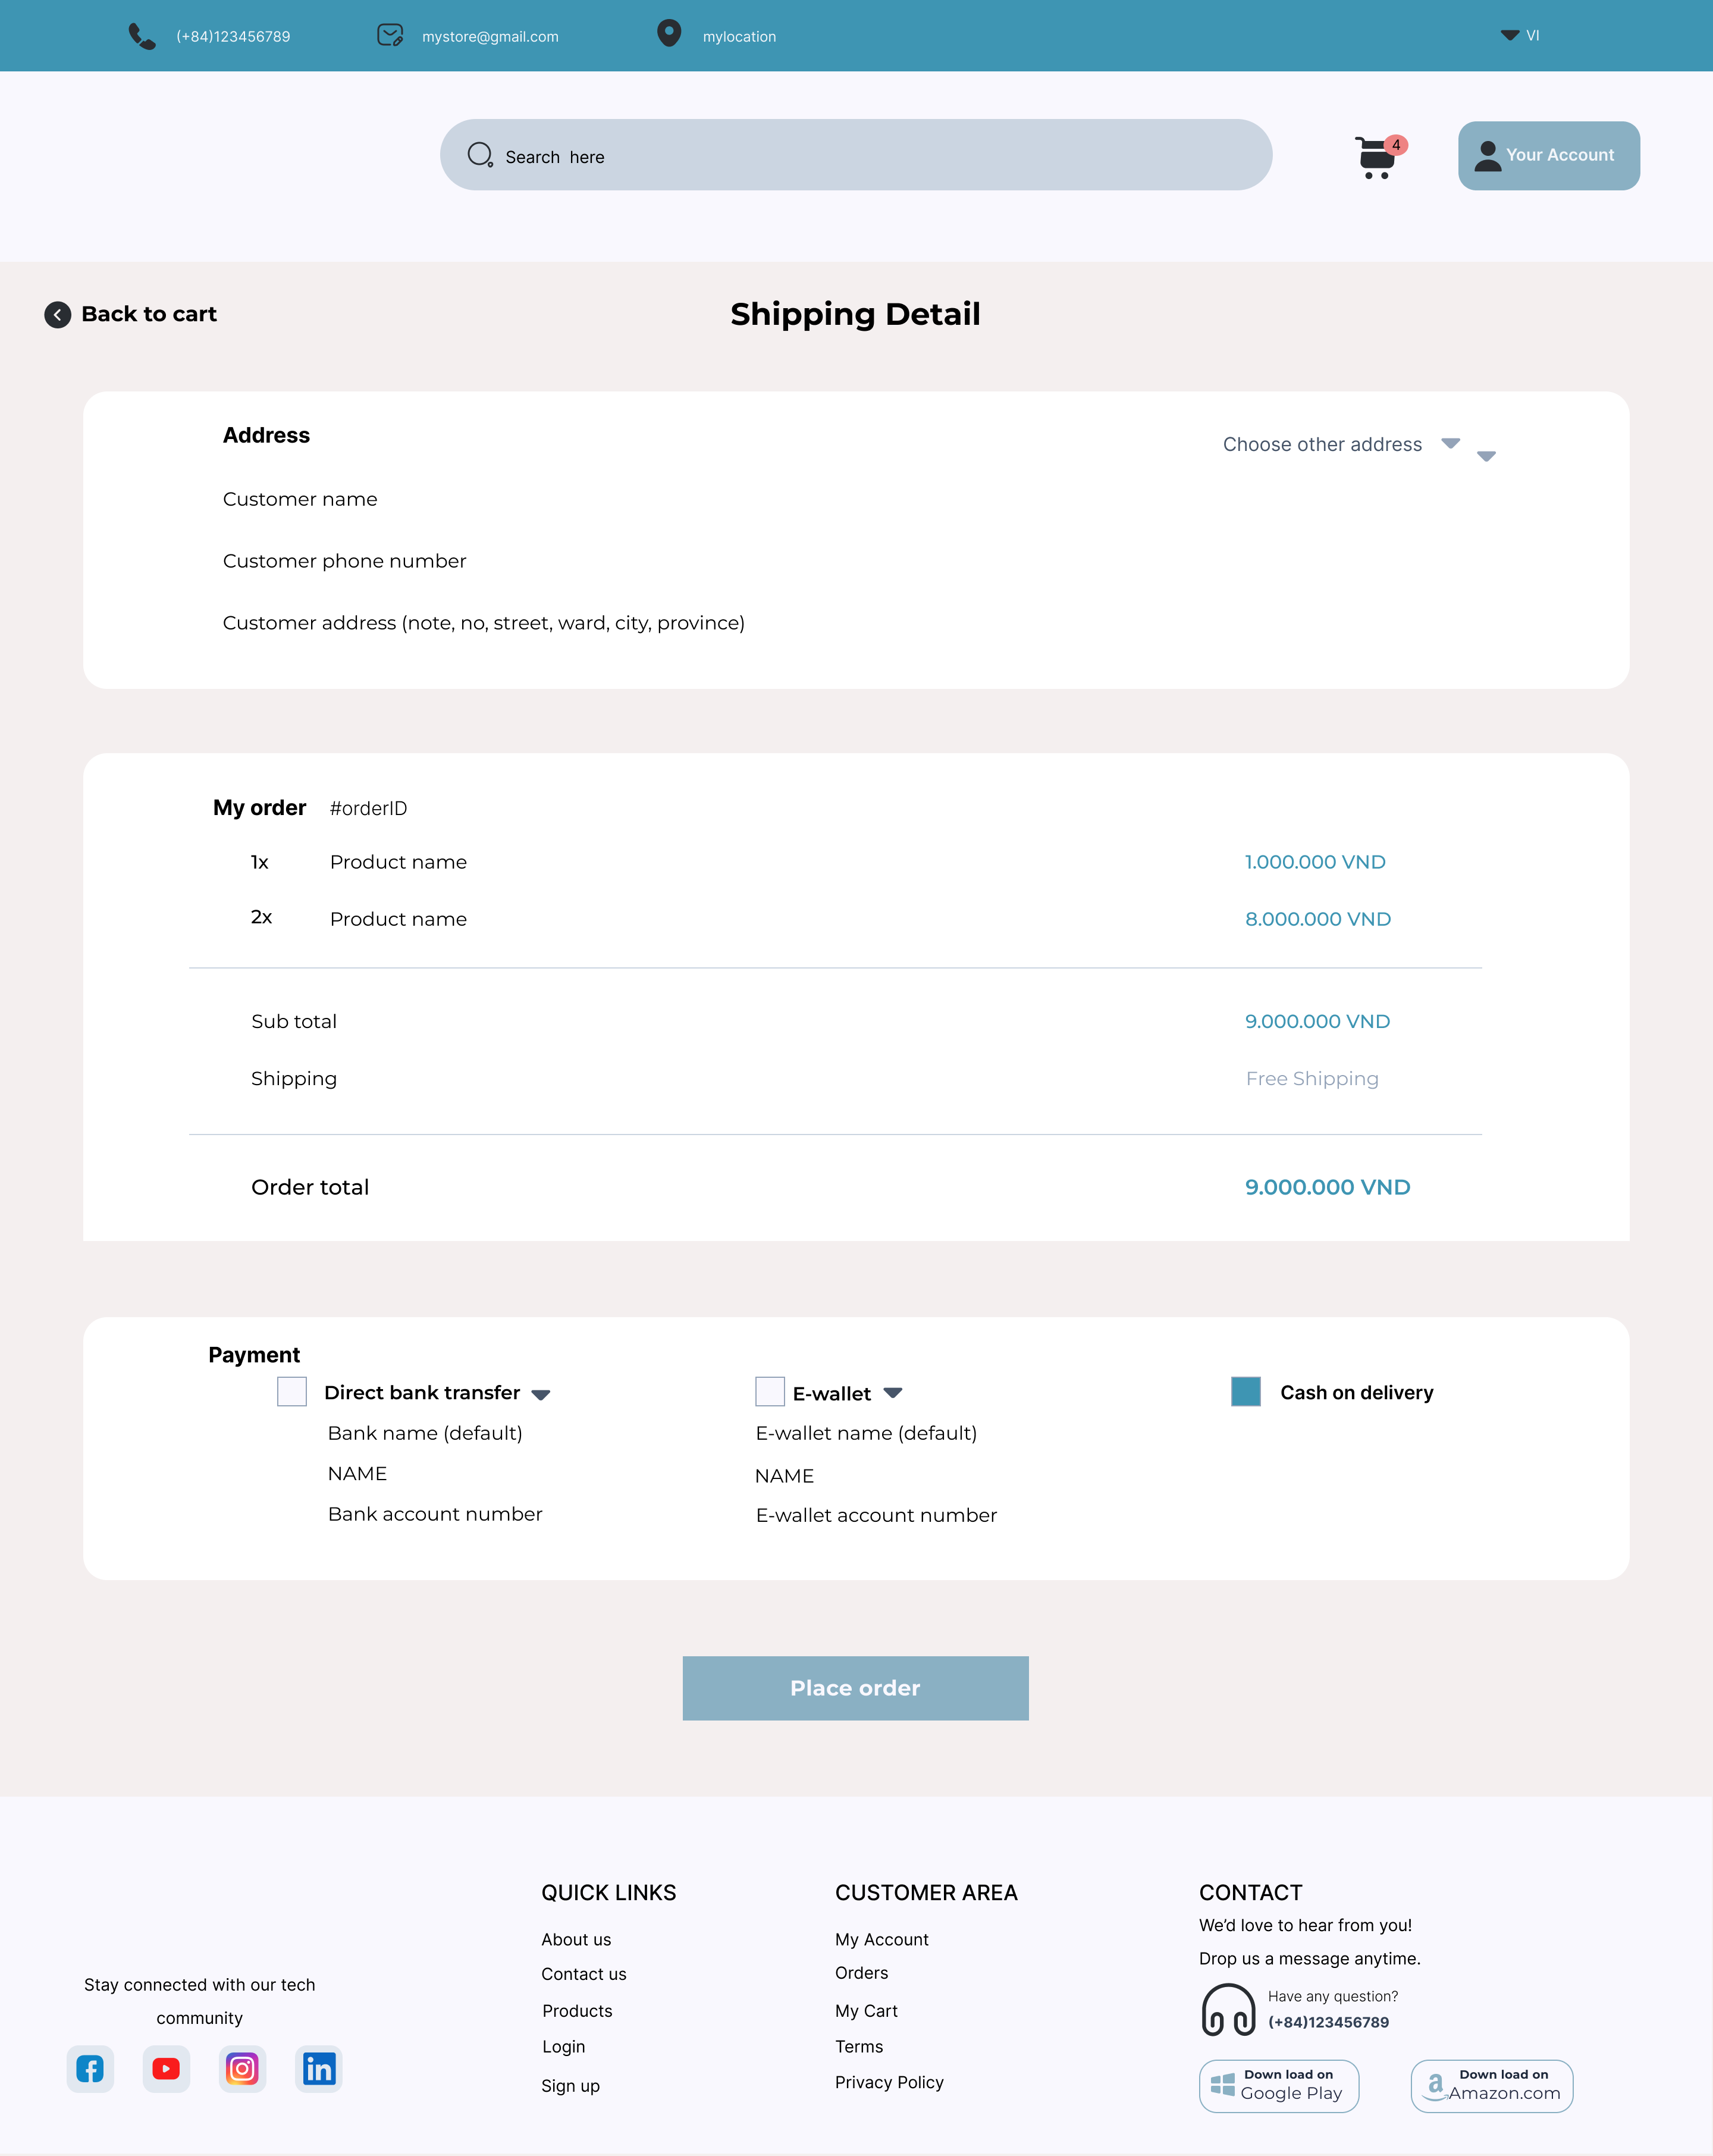
\includegraphics[width=0.9\linewidth]{images/ui/ui_shipping_detail.png}
   \vspace{0.5cm} \caption{Giao diện Thông tin giao hàng}
    \label{fig:ui_shipping}
\end{figure}
Bước nhập địa chỉ nhận hàng và chọn phương thức vận chuyển. Hệ thống có thể gợi ý địa chỉ đã lưu nếu người dùng đã đăng nhập.

% --- NHÓM 4: QUẢN LÝ TÀI KHOẢN (USER PROFILE) ---

\begin{figure}[H]
    \centering
    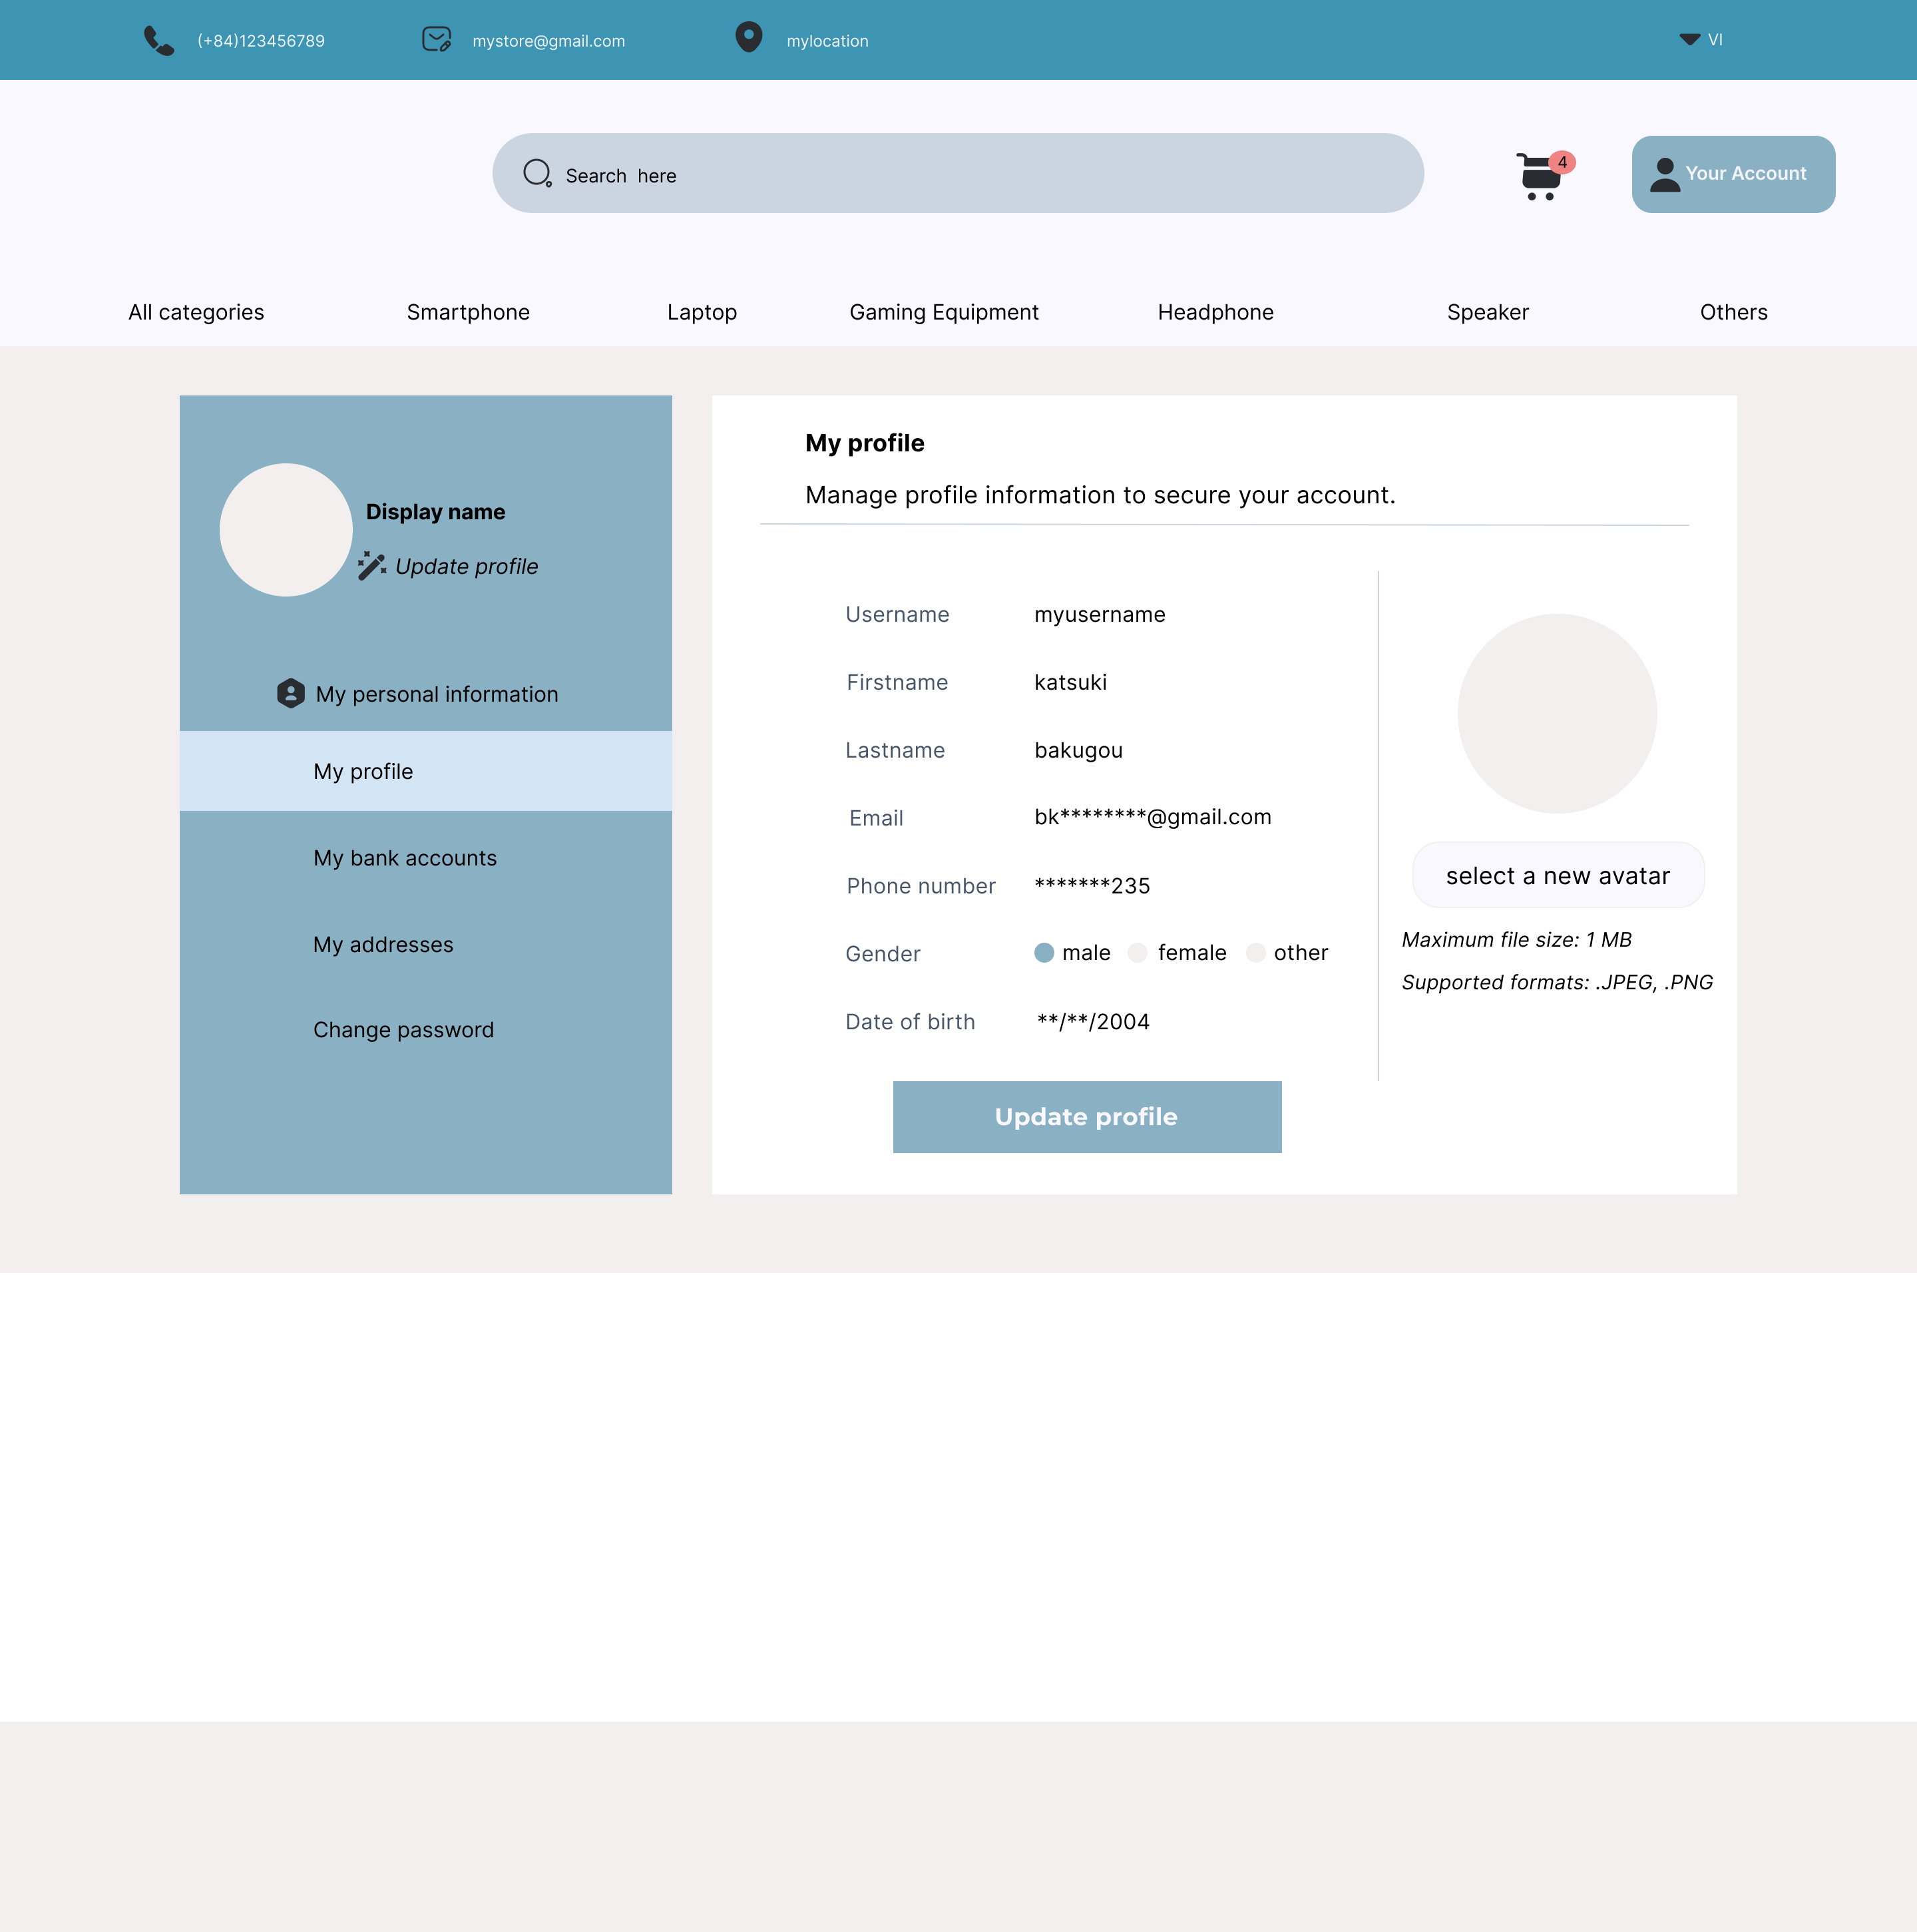
\includegraphics[width=0.8\linewidth]{images/ui/ui_view_profile_profile.png}
   \vspace{0.5cm} \caption{Giao diện Hồ sơ cá nhân}
    \label{fig:ui_profile_info}
\end{figure}
Nơi người dùng xem và cập nhật thông tin định danh cơ bản như Họ tên, Số điện thoại, Email liên hệ.

\begin{figure}[H]
    \centering
    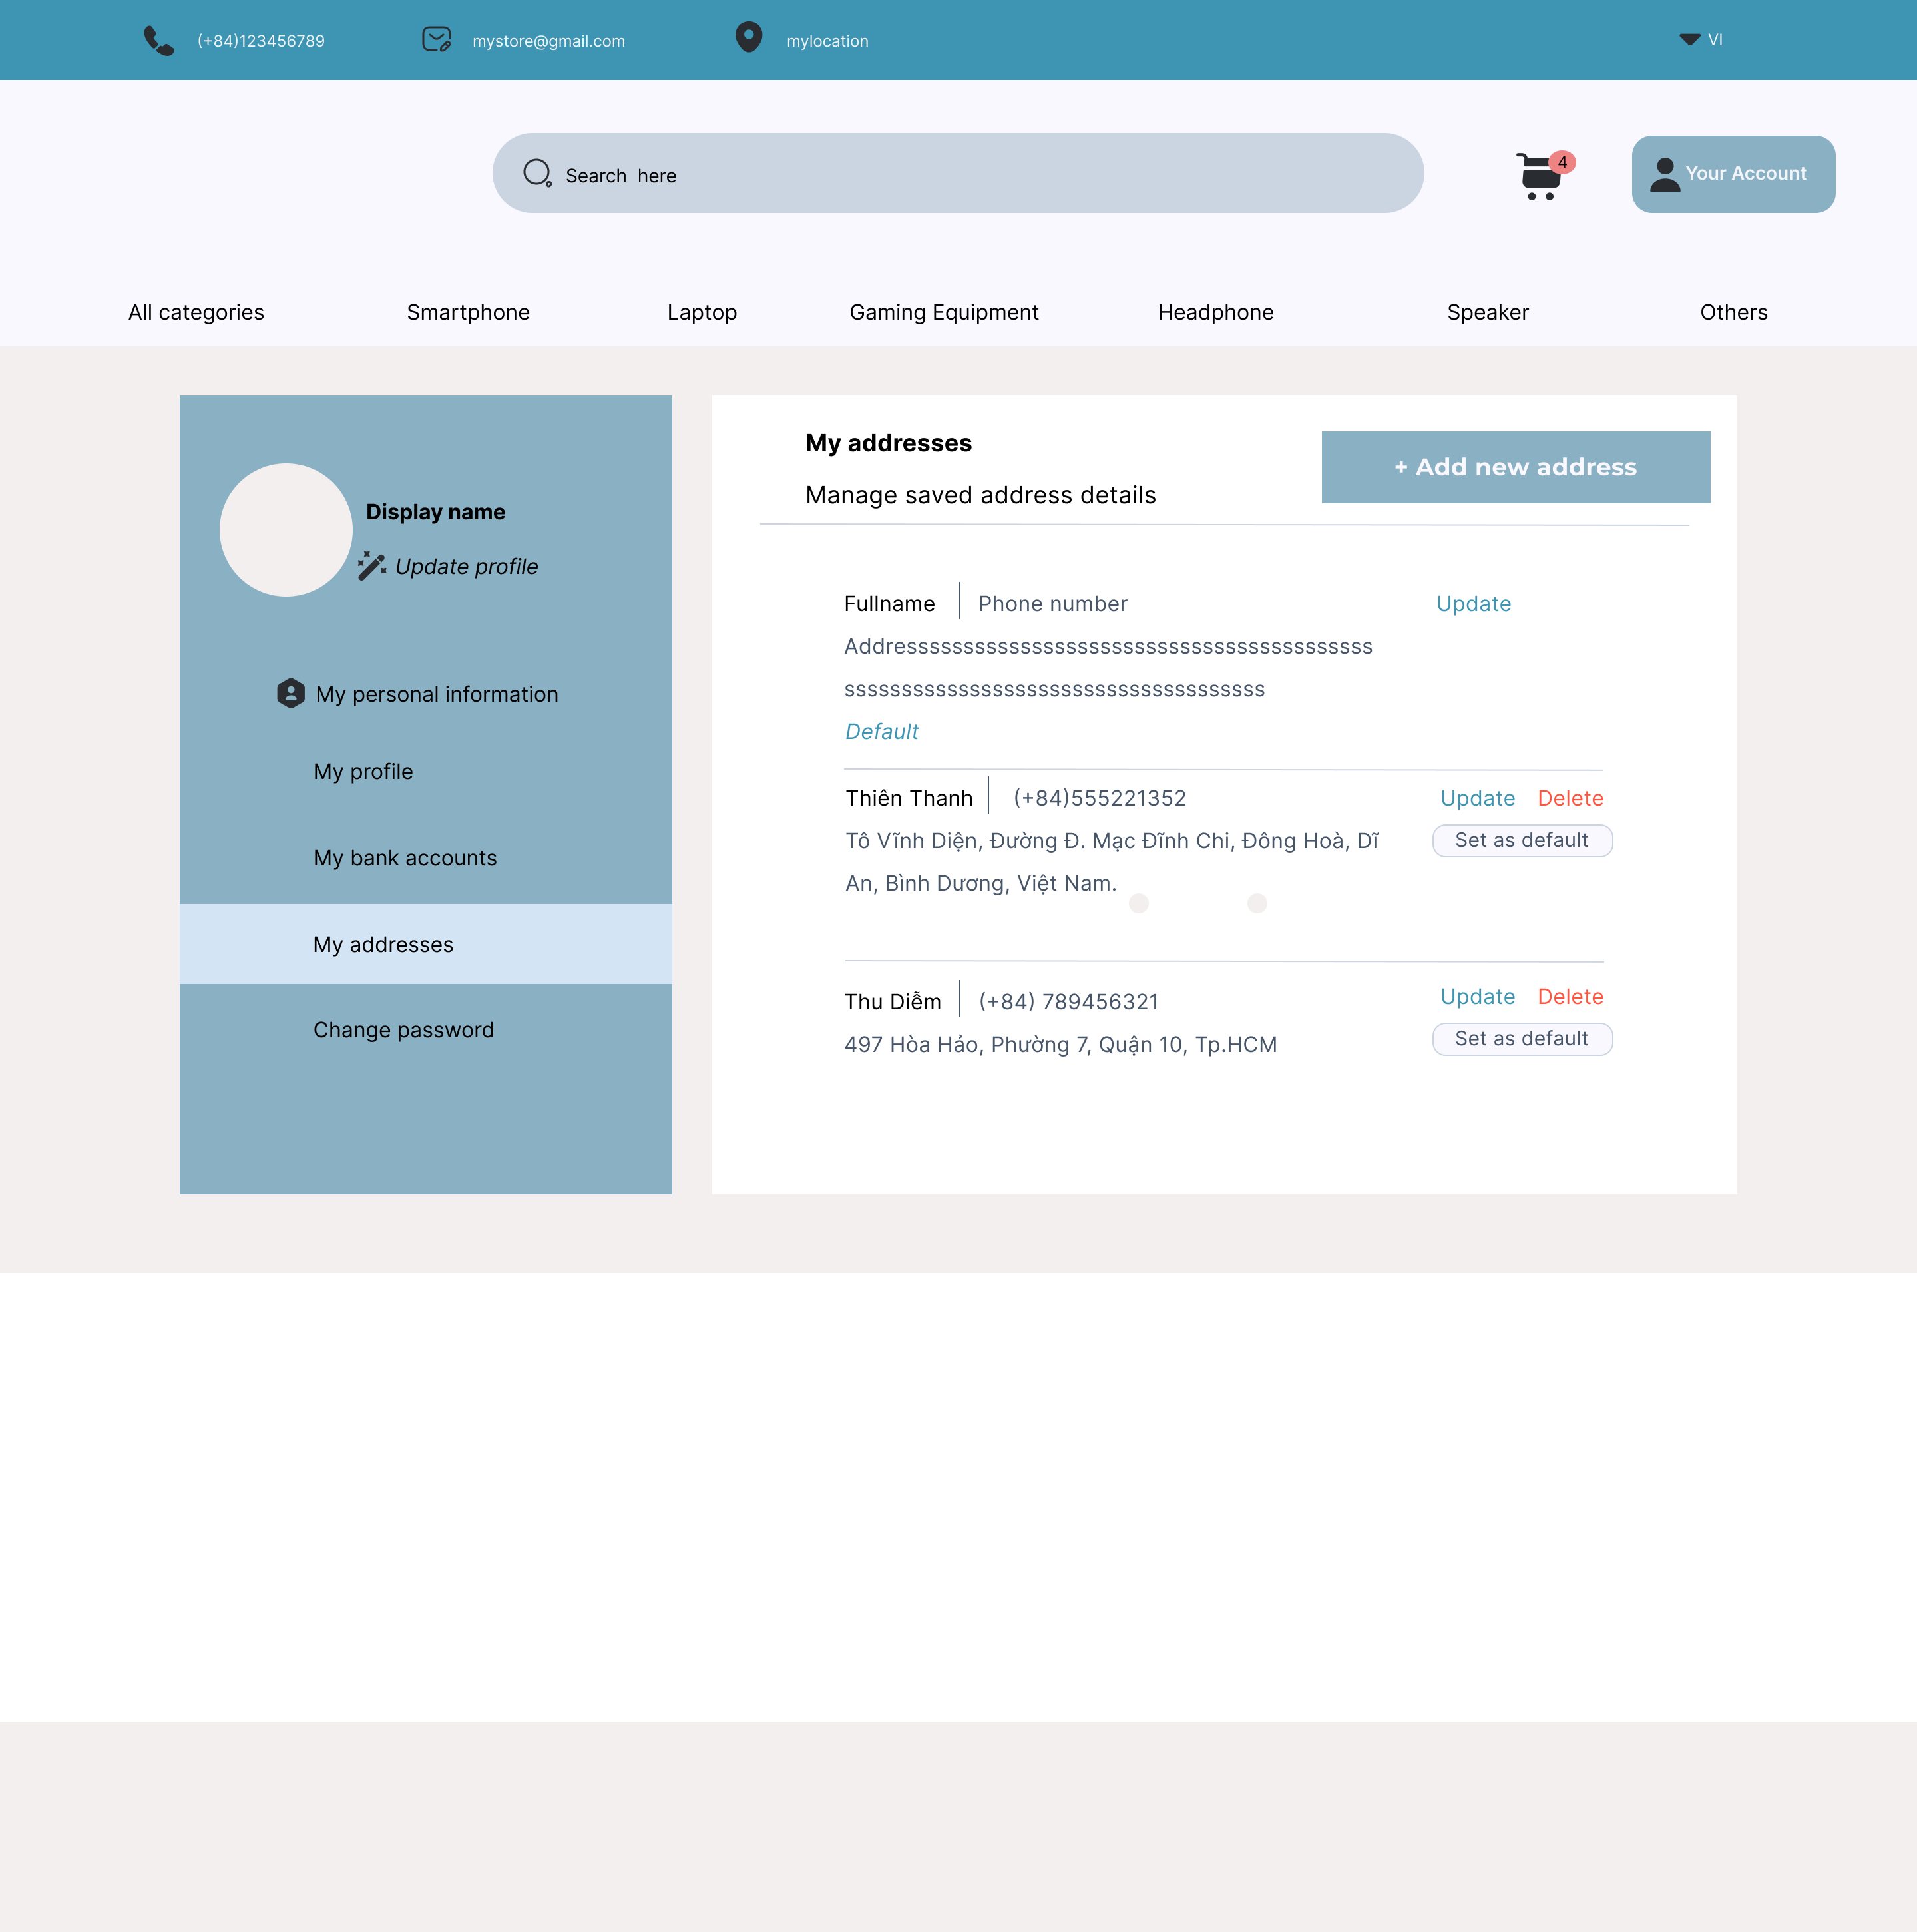
\includegraphics[width=0.8\linewidth]{images/ui/ui_view_profile_address.png}
   \vspace{0.5cm} \caption{Giao diện Sổ địa chỉ}
    \label{fig:ui_profile_address}
\end{figure}
Quản lý danh sách các địa chỉ giao hàng (Nhà riêng, Cơ quan), cho phép thêm mới hoặc đặt địa chỉ mặc định để rút ngắn thời gian thanh toán cho các lần sau.

\begin{figure}[H]
    \centering
    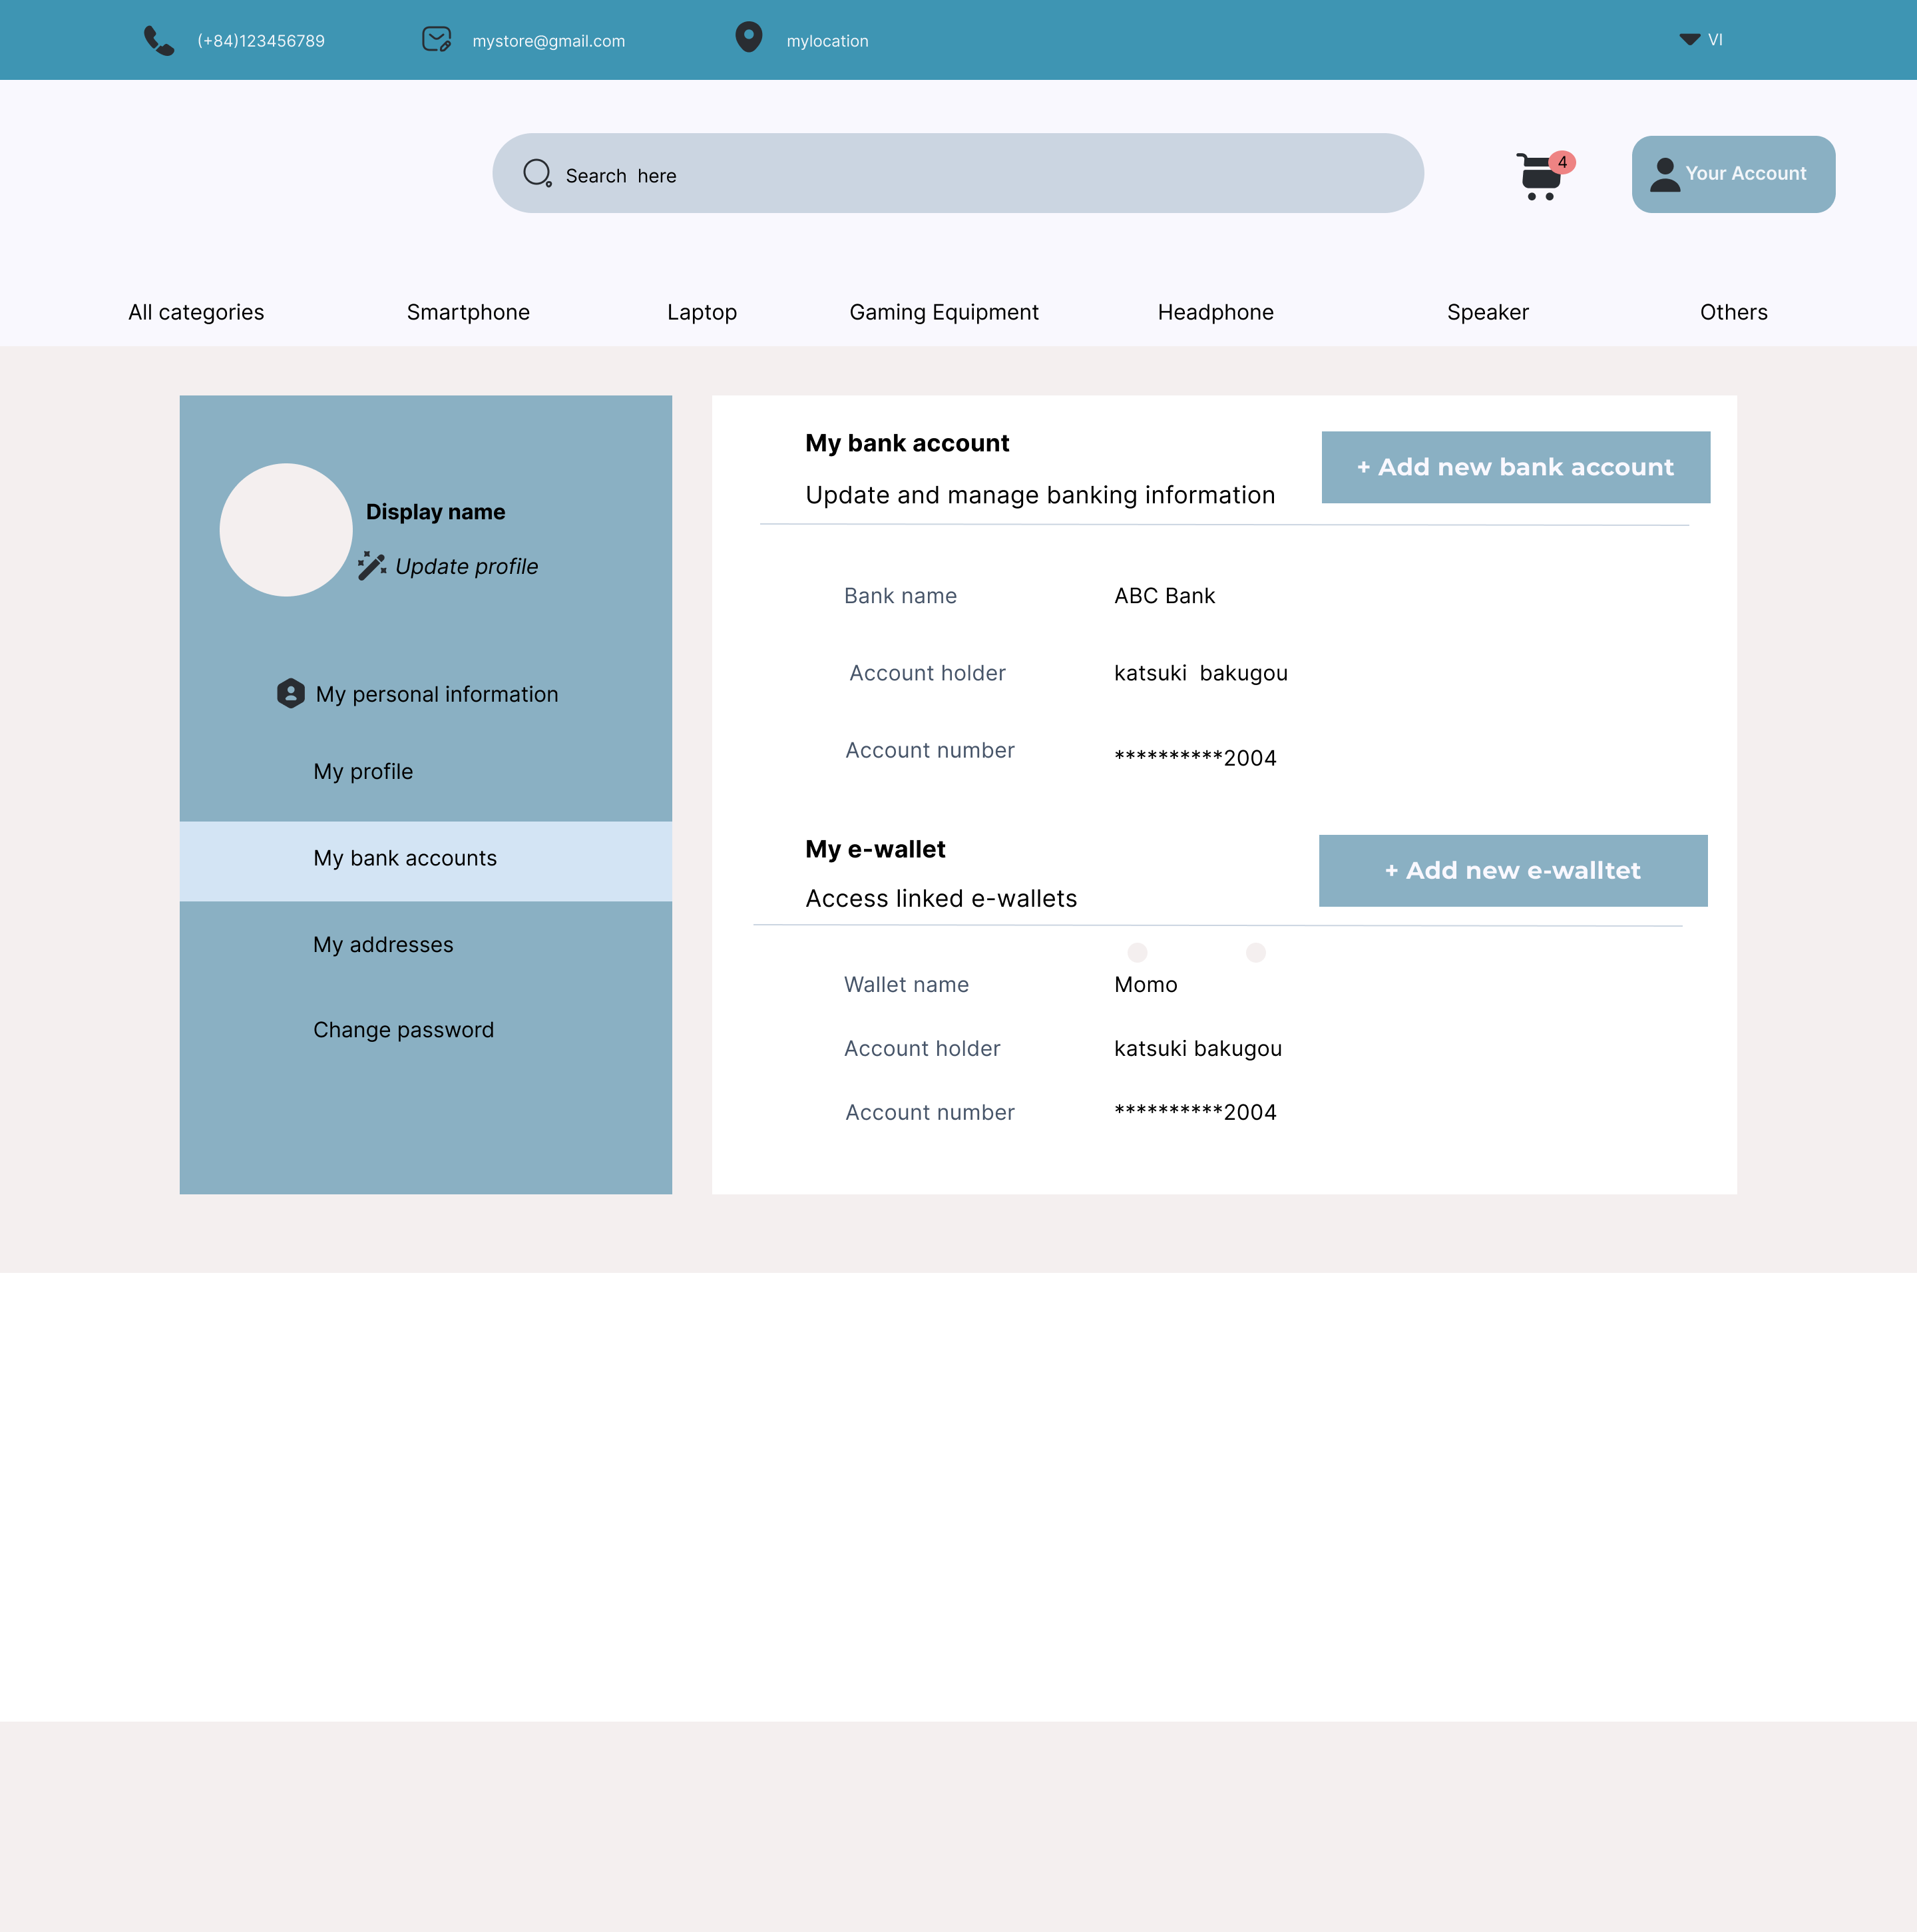
\includegraphics[width=0.8\linewidth]{images/ui/ui_view_profile_bank.png}
   \vspace{0.5cm} \caption{Giao diện Tài khoản ngân hàng liên kết}
    \label{fig:ui_profile_bank}
\end{figure}
Quản lý các phương thức thanh toán đã lưu hoặc tài khoản ngân hàng dùng cho việc hoàn tiền (nếu có phát sinh trả hàng).

\begin{figure}[H]
    \centering
    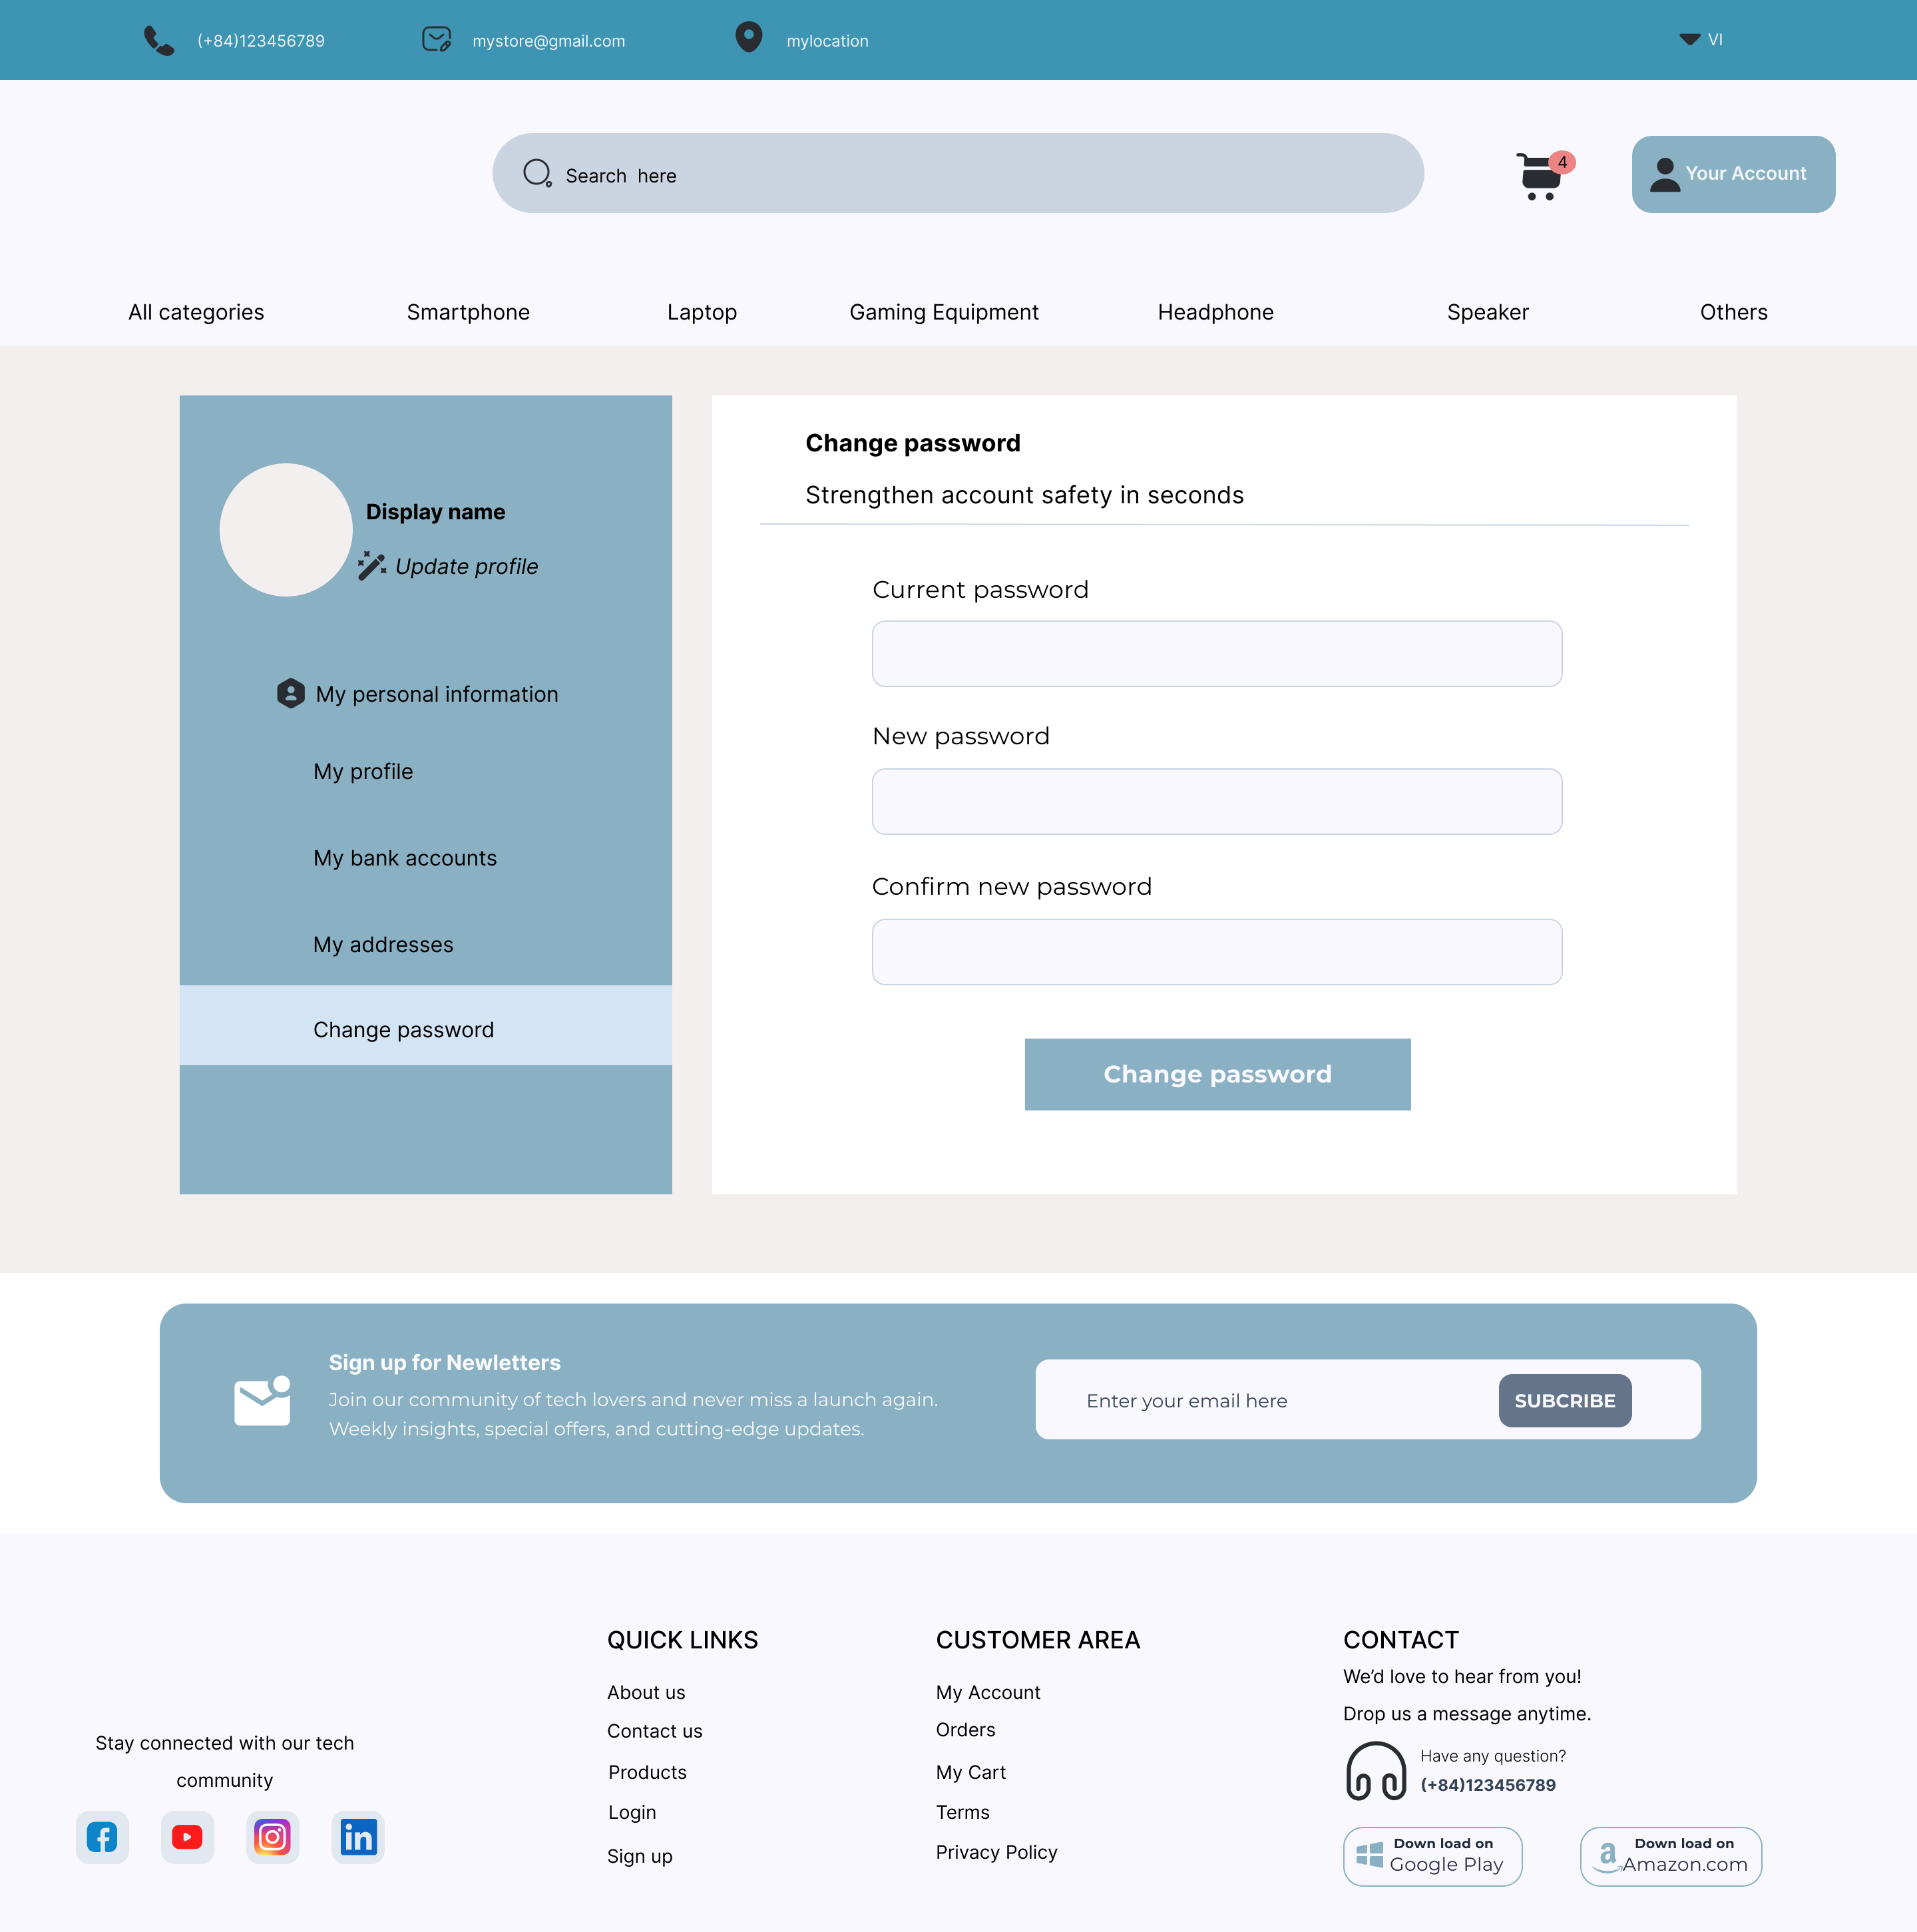
\includegraphics[width=0.8\linewidth]{images/ui/ui_view_profile_change_password.png}
   \vspace{0.5cm} \caption{Giao diện Đổi mật khẩu}
    \label{fig:ui_change_pass}
\end{figure}
Tính năng bảo mật cho phép người dùng thay đổi mật khẩu định kỳ để bảo vệ tài khoản.

% --- NHÓM 5: QUẢN LÝ ĐƠN HÀNG (ORDER MANAGEMENT) ---

\begin{figure}[H]
    \centering
    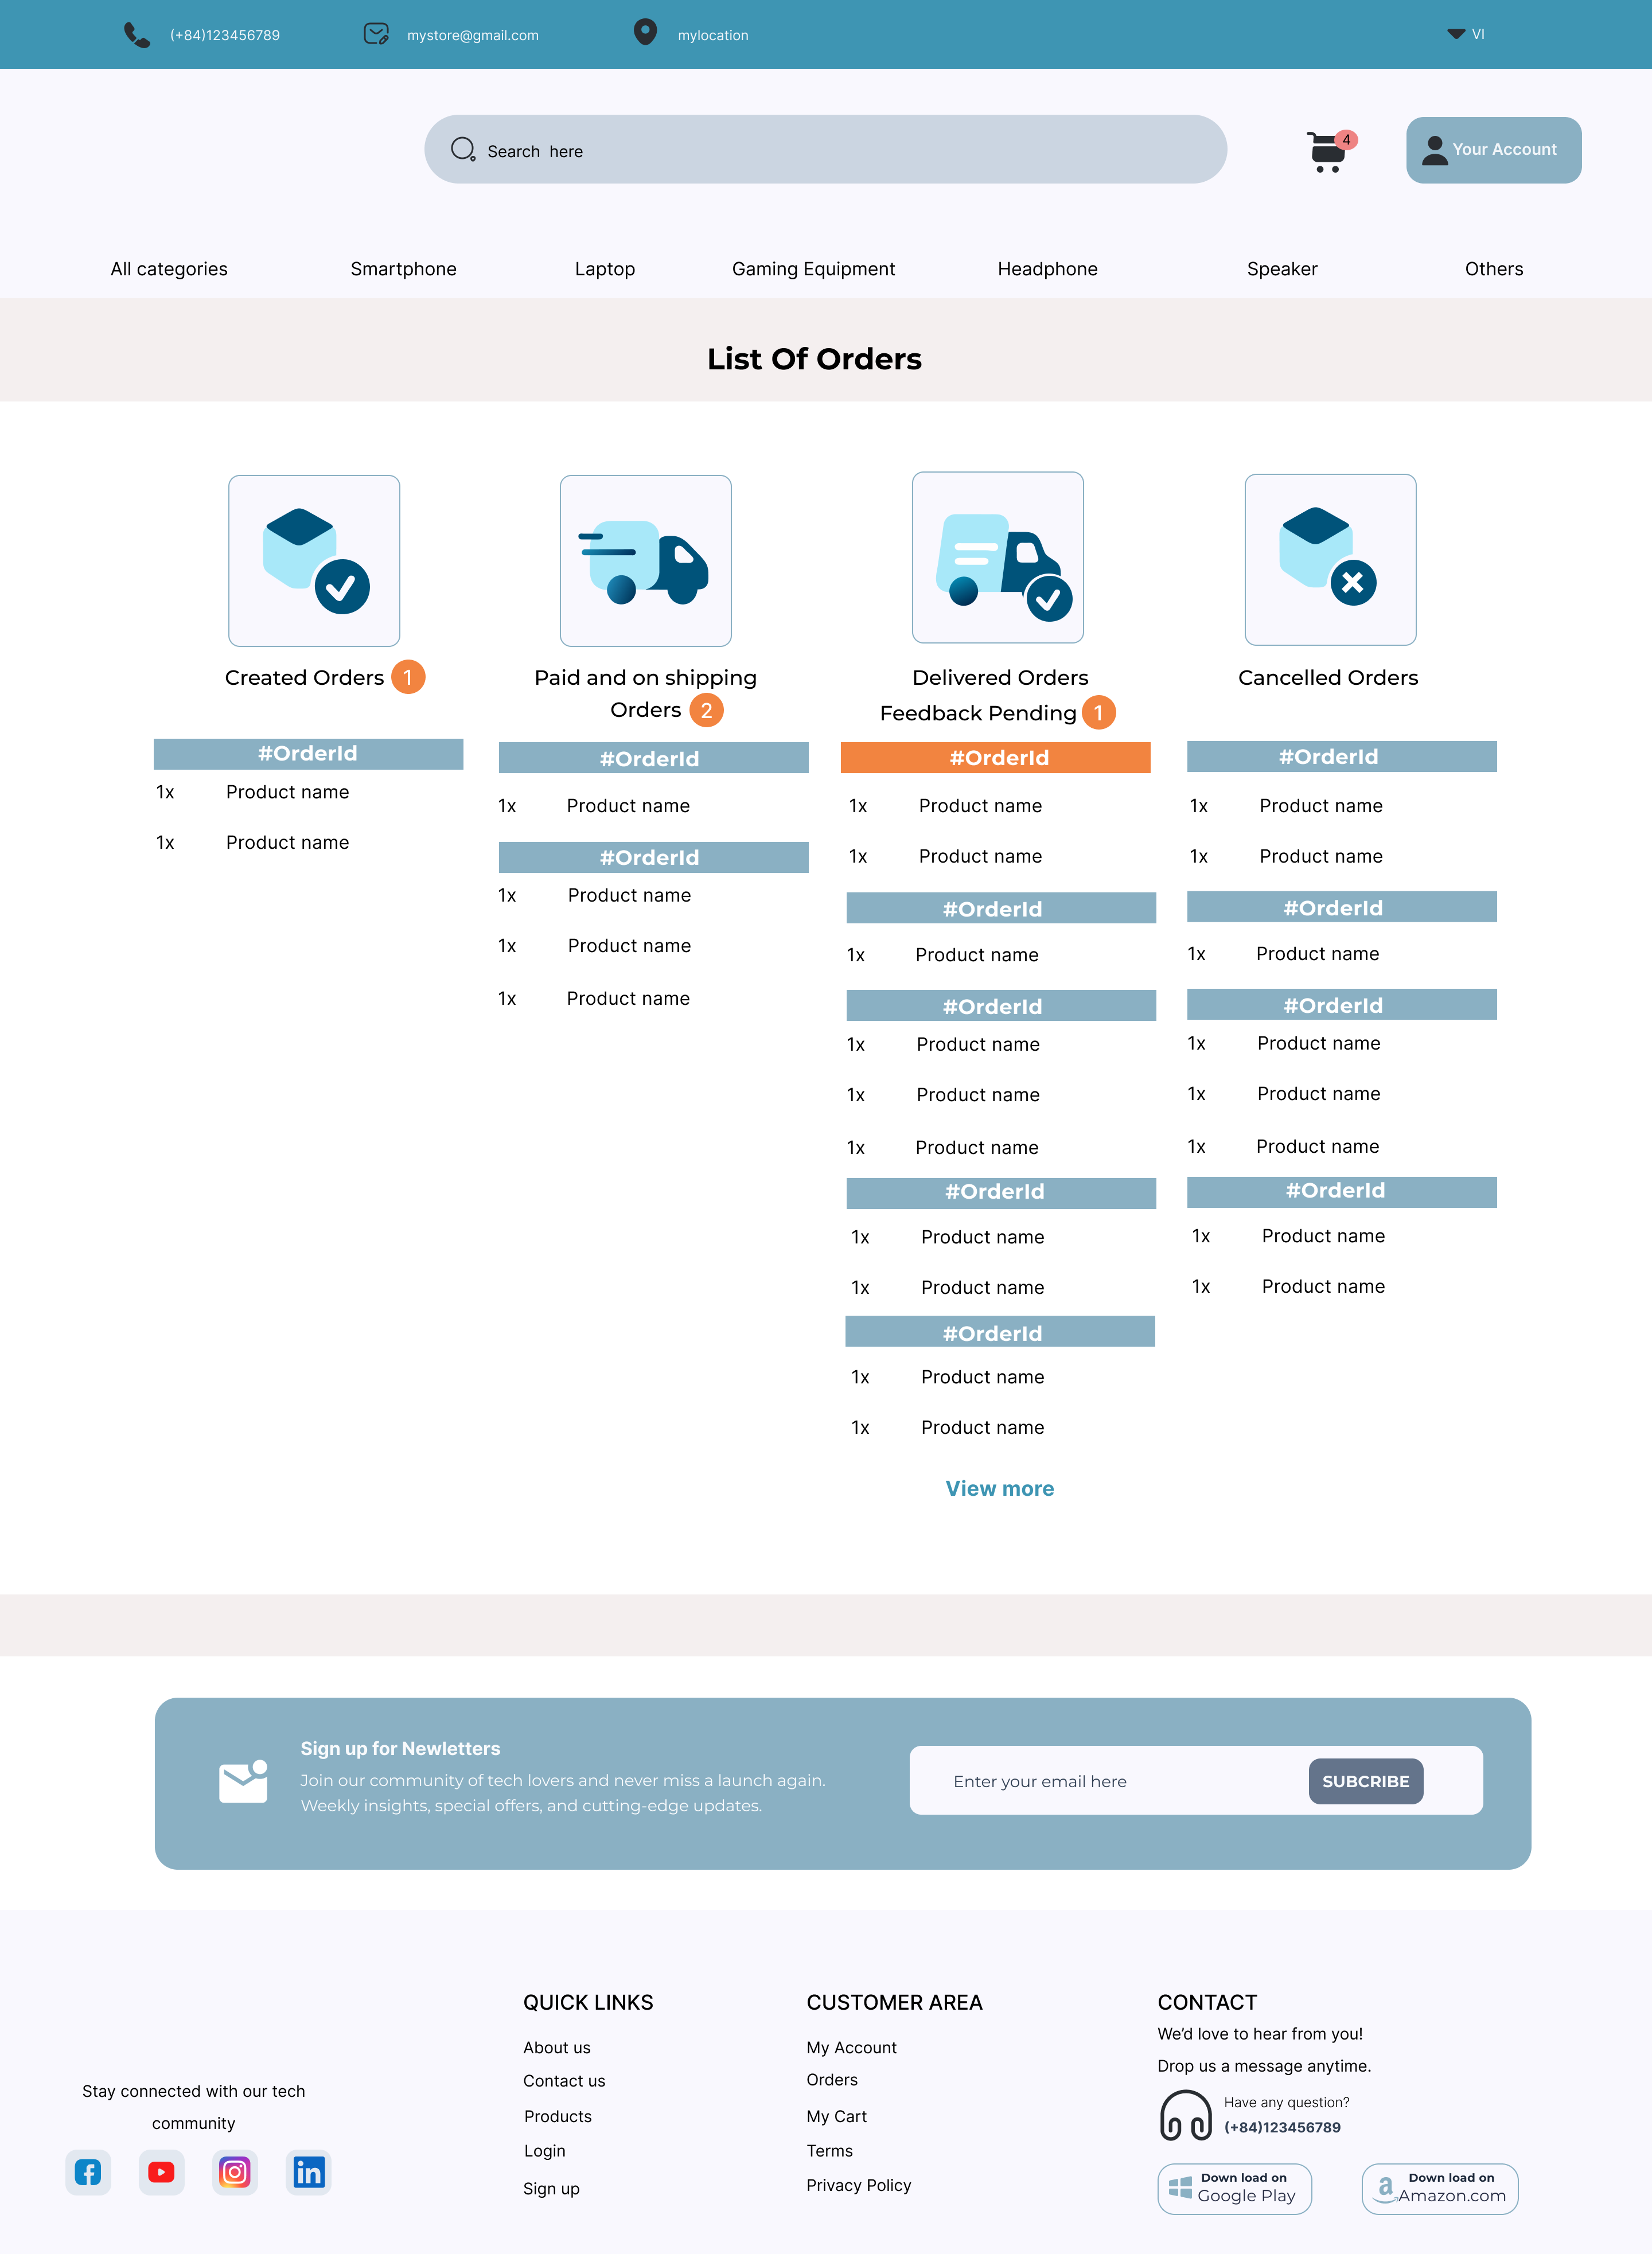
\includegraphics[width=0.9\linewidth]{images/ui/ui_list_of_order.png}
   \vspace{0.5cm} \caption{Giao diện Lịch sử đơn hàng}
    \label{fig:ui_order_list}
\end{figure}
Danh sách liệt kê tất cả đơn hàng đã đặt, được phân loại theo trạng thái (Chờ xác nhận, Đang giao, Đã giao, Đã hủy) giúp người dùng dễ dàng theo dõi.

\begin{figure}[H]
    \centering
    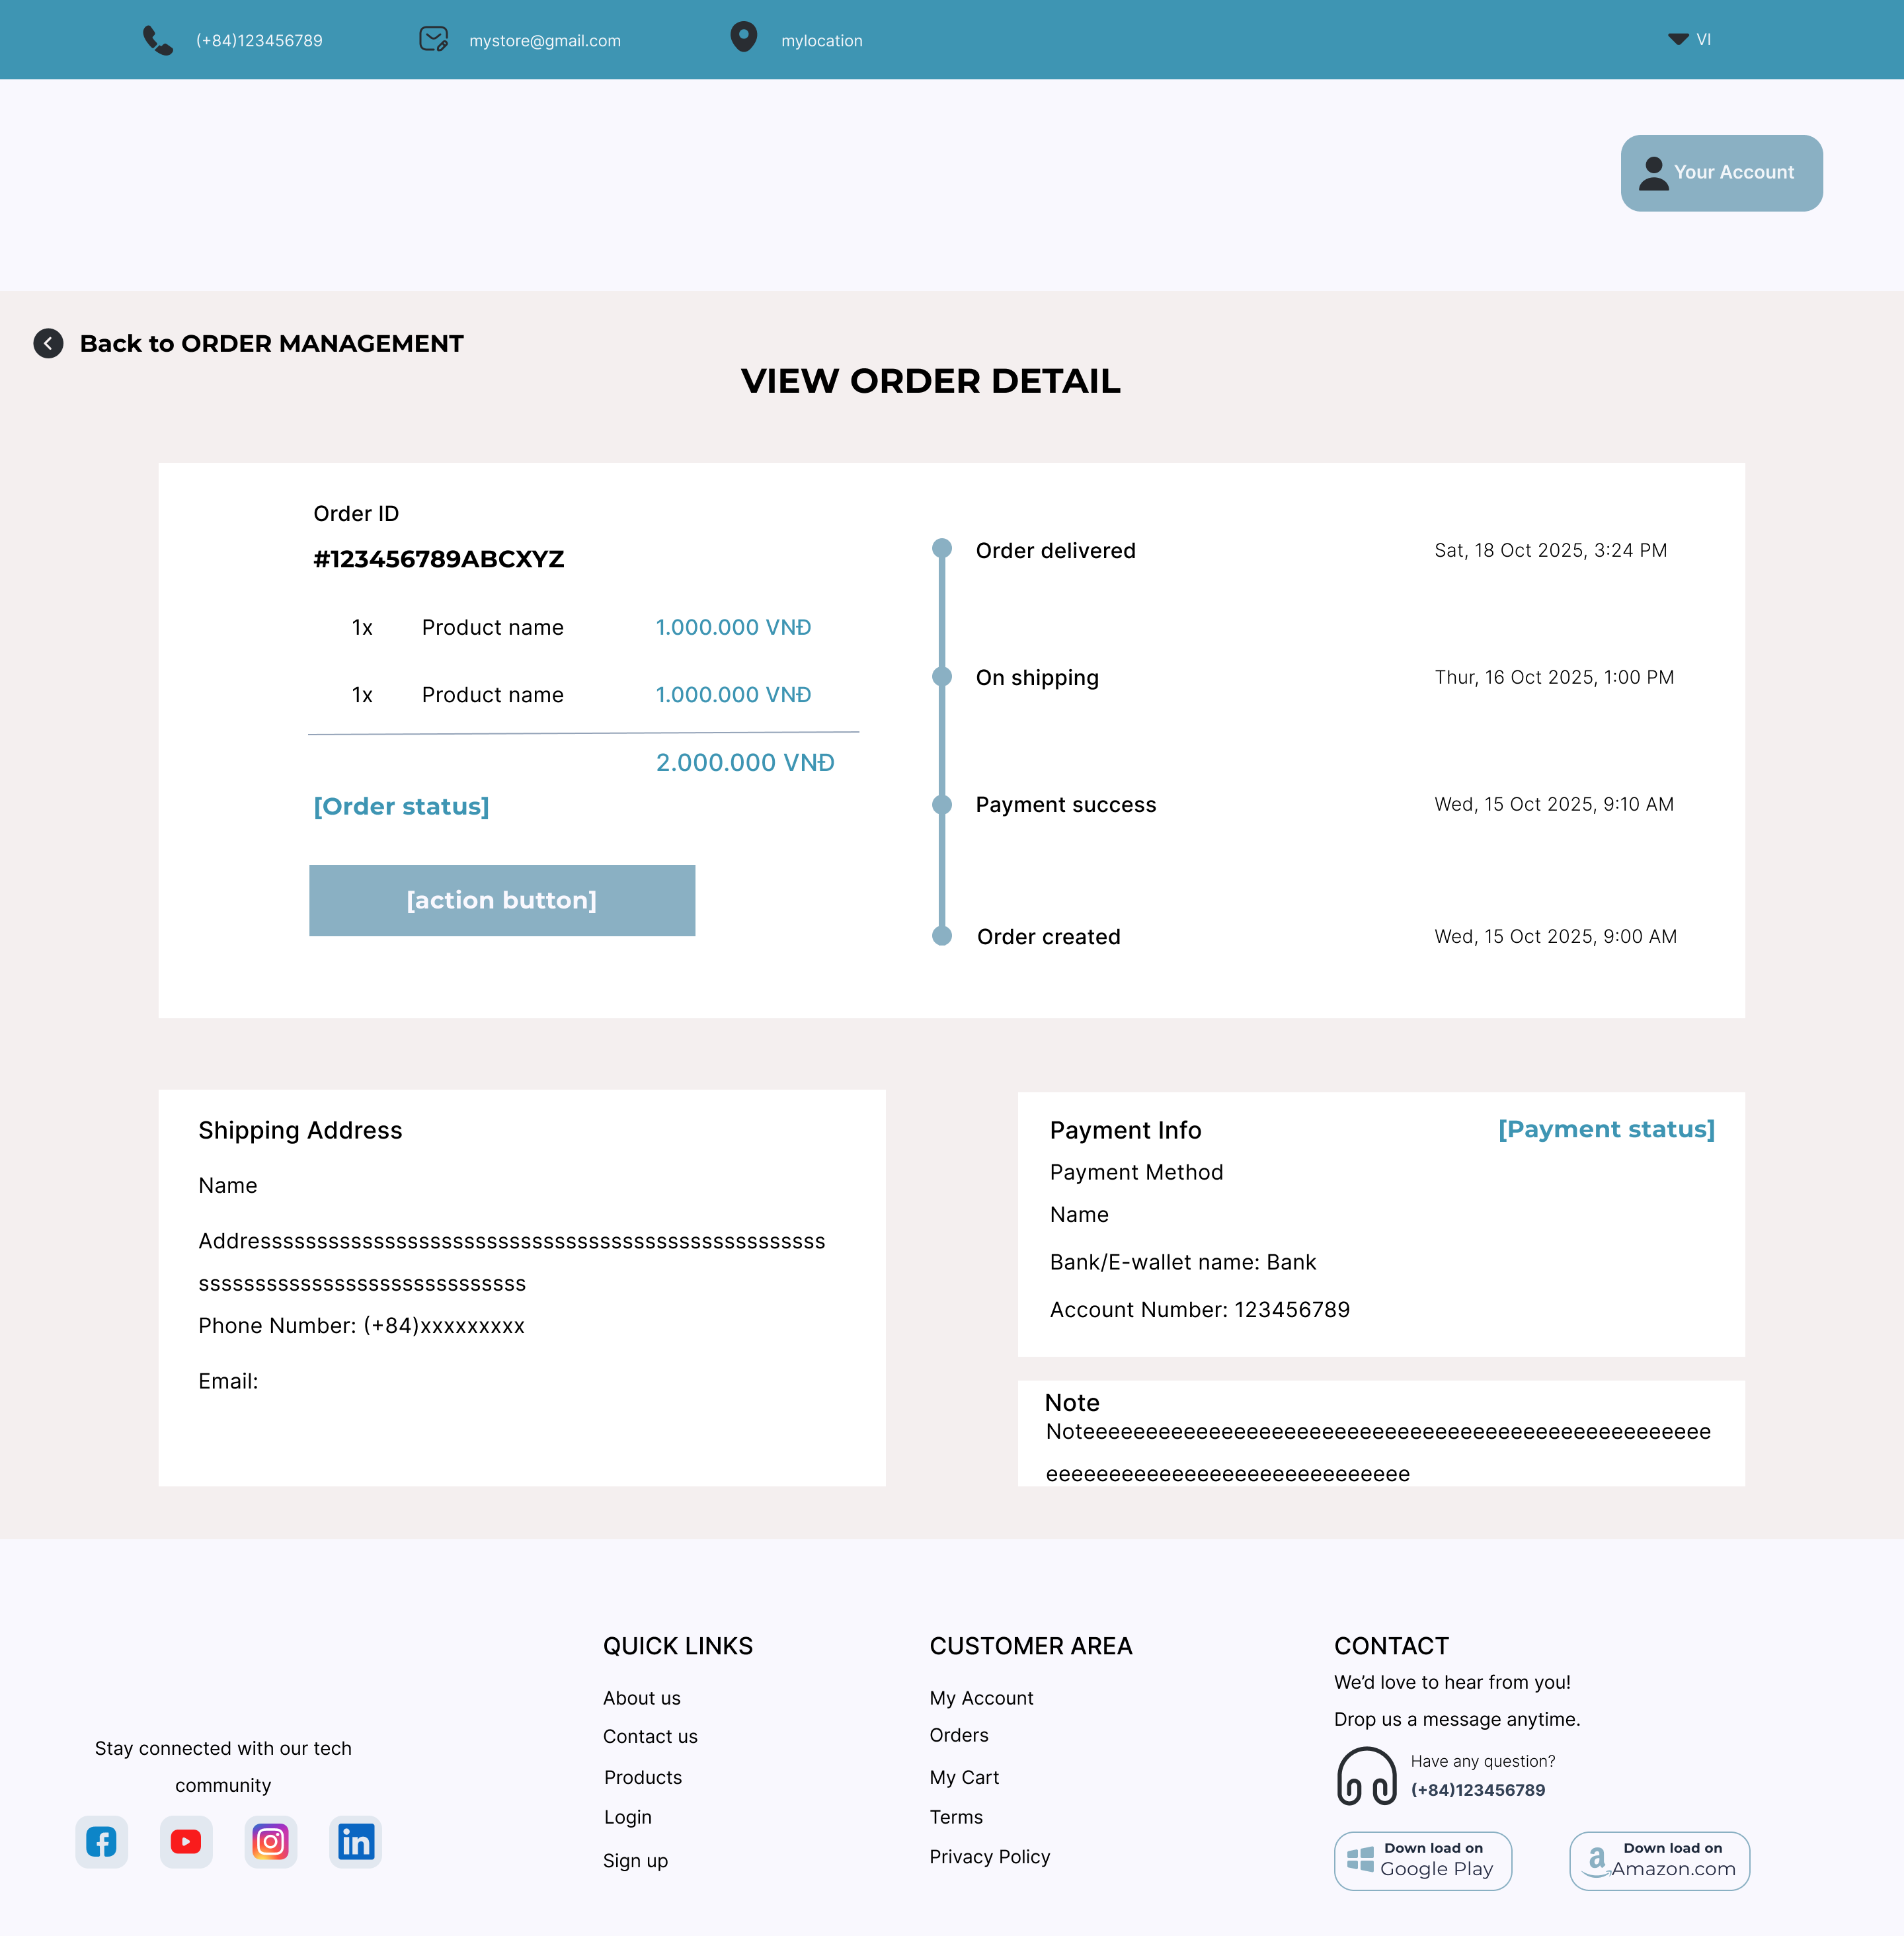
\includegraphics[width=0.9\linewidth]{images/ui/ui_order_detail.png}
   \vspace{0.5cm} \caption{Giao diện Chi tiết đơn hàng}
    \label{fig:ui_order_detail}
\end{figure}
Hiển thị đầy đủ thông tin của một đơn hàng cụ thể: Danh sách sản phẩm, tổng tiền, thông tin người nhận và mã vận đơn.

\begin{figure}[H]
    \centering
    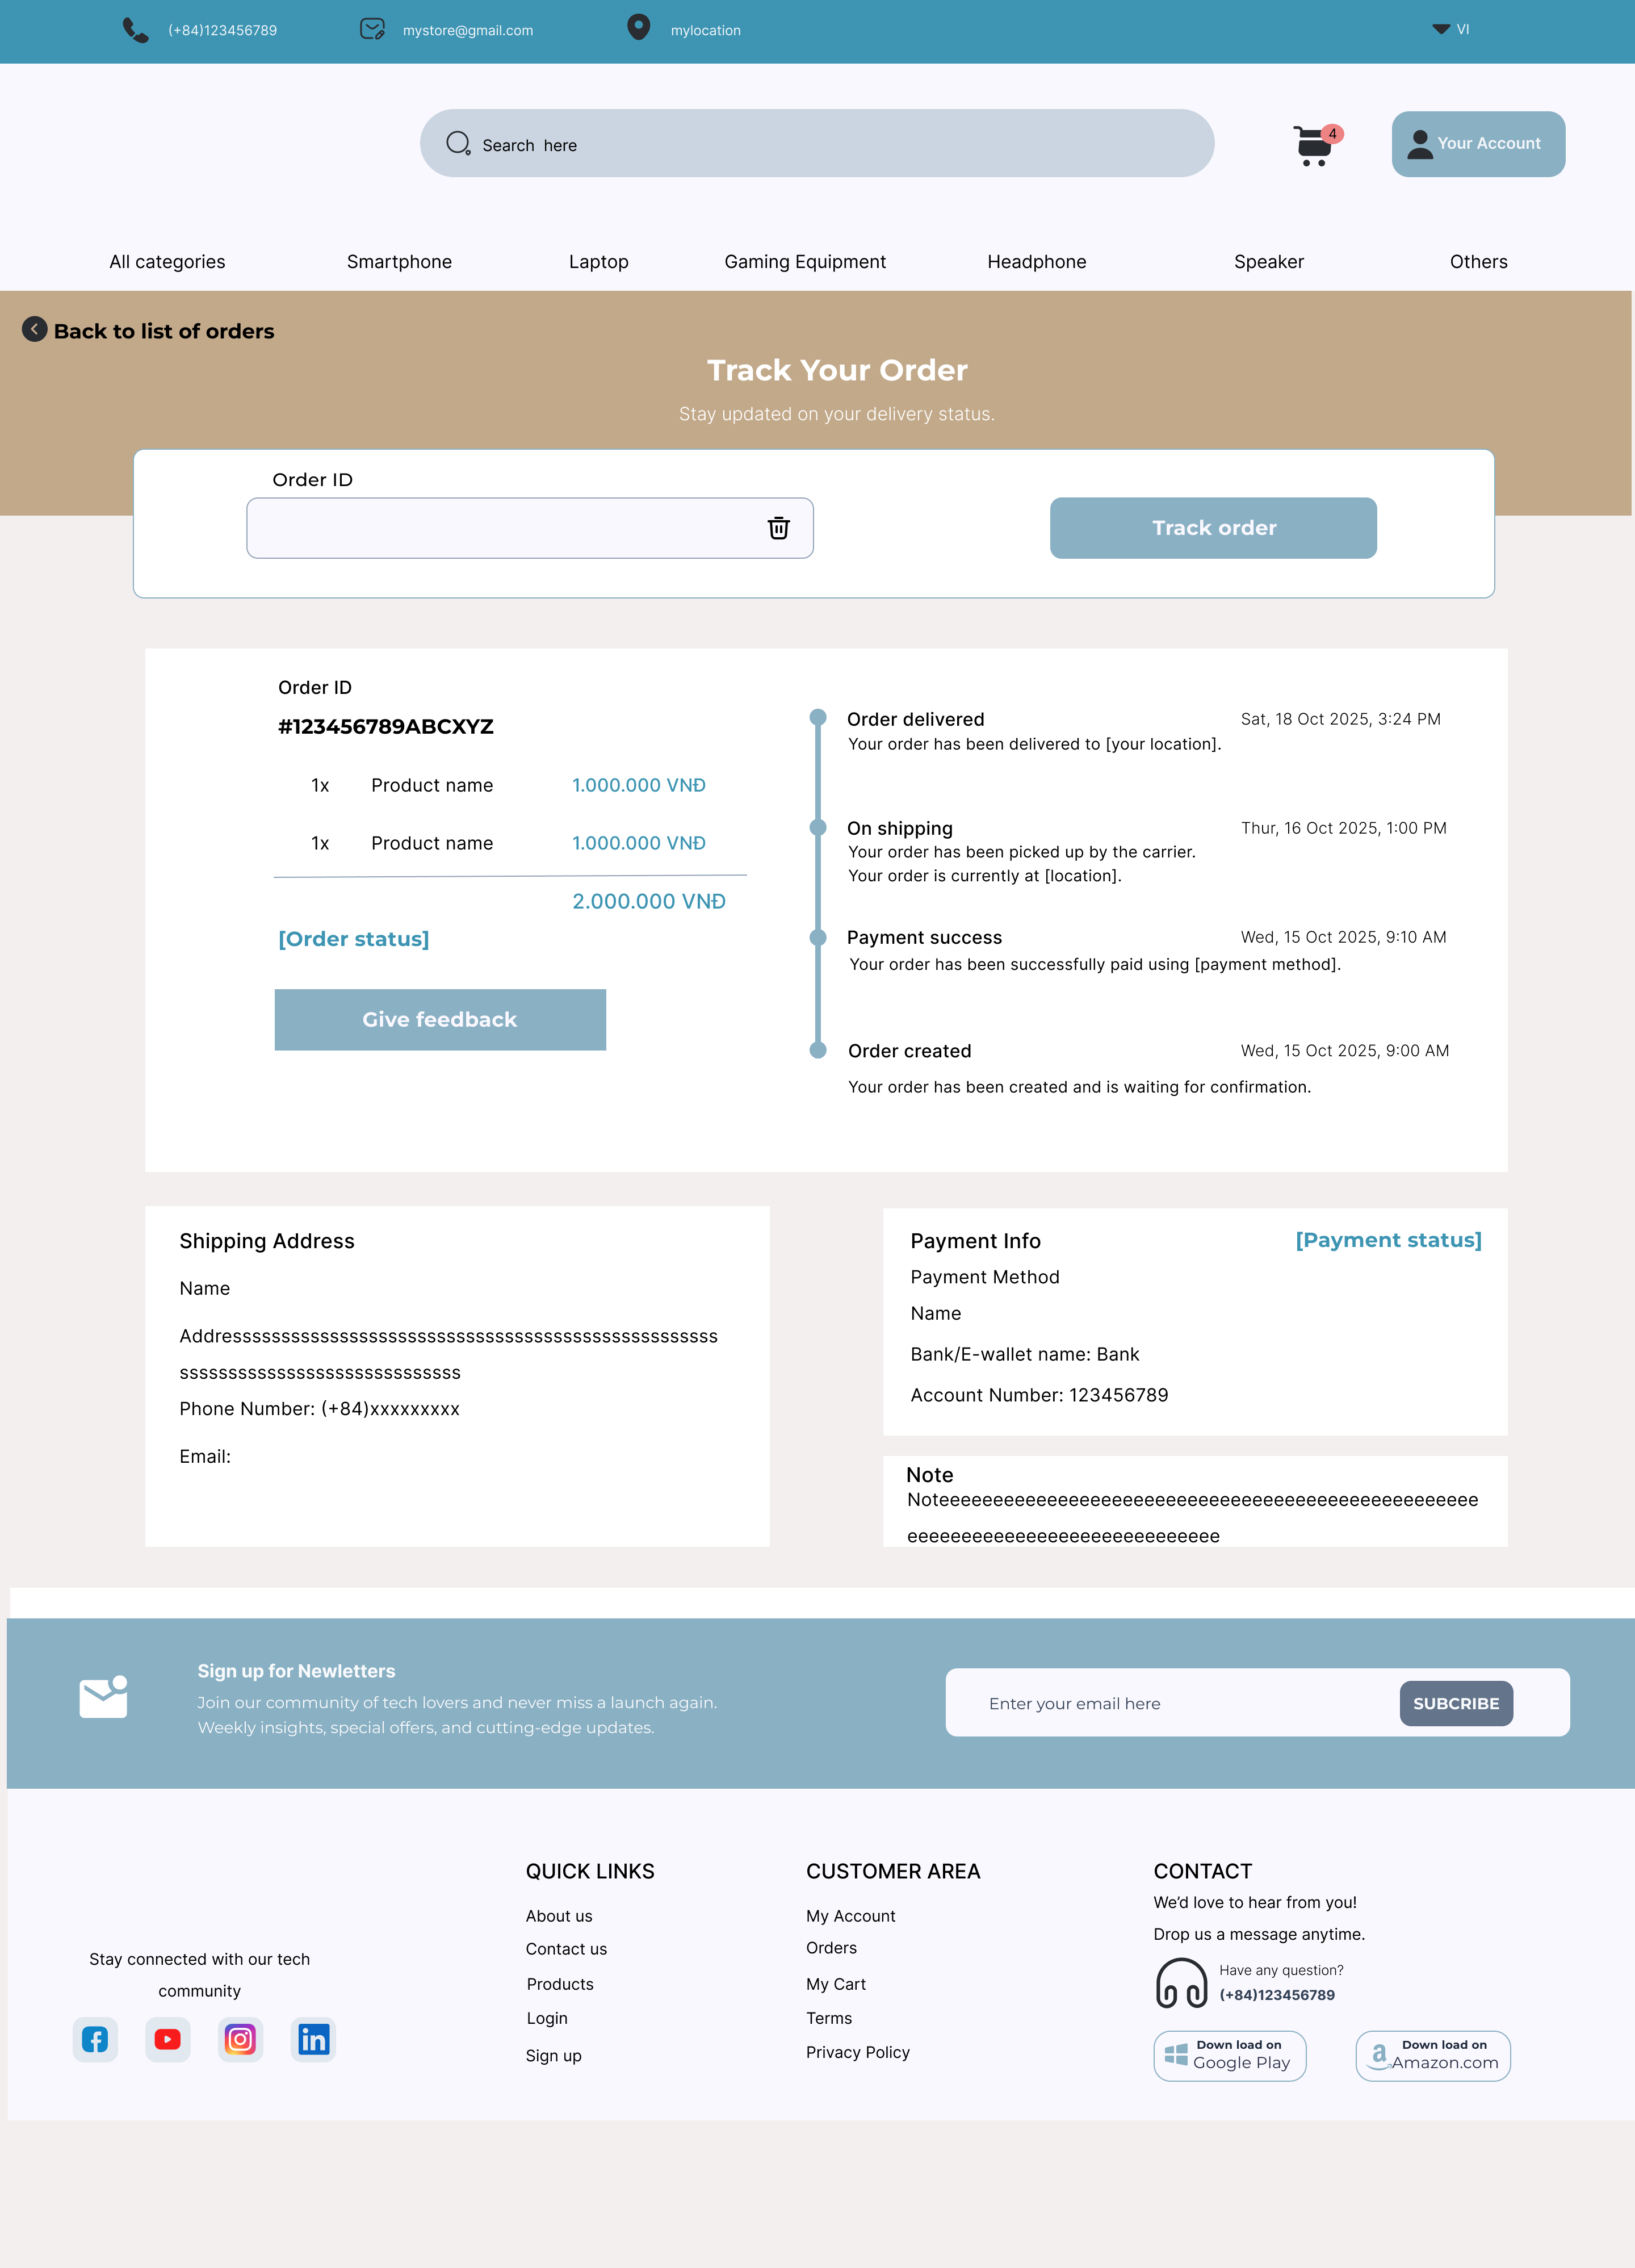
\includegraphics[width=0.9\linewidth]{images/ui/ui_tracking_order.png}
   \vspace{0.5cm} \caption{Giao diện Theo dõi đơn hàng (Tracking)}
    \label{fig:ui_tracking}
\end{figure}
Biểu đồ dòng thời gian (Timeline) trực quan hiển thị hành trình của gói hàng từ lúc xuất kho đến khi giao tới tay khách hàng.

\begin{figure}[H]
    \centering
    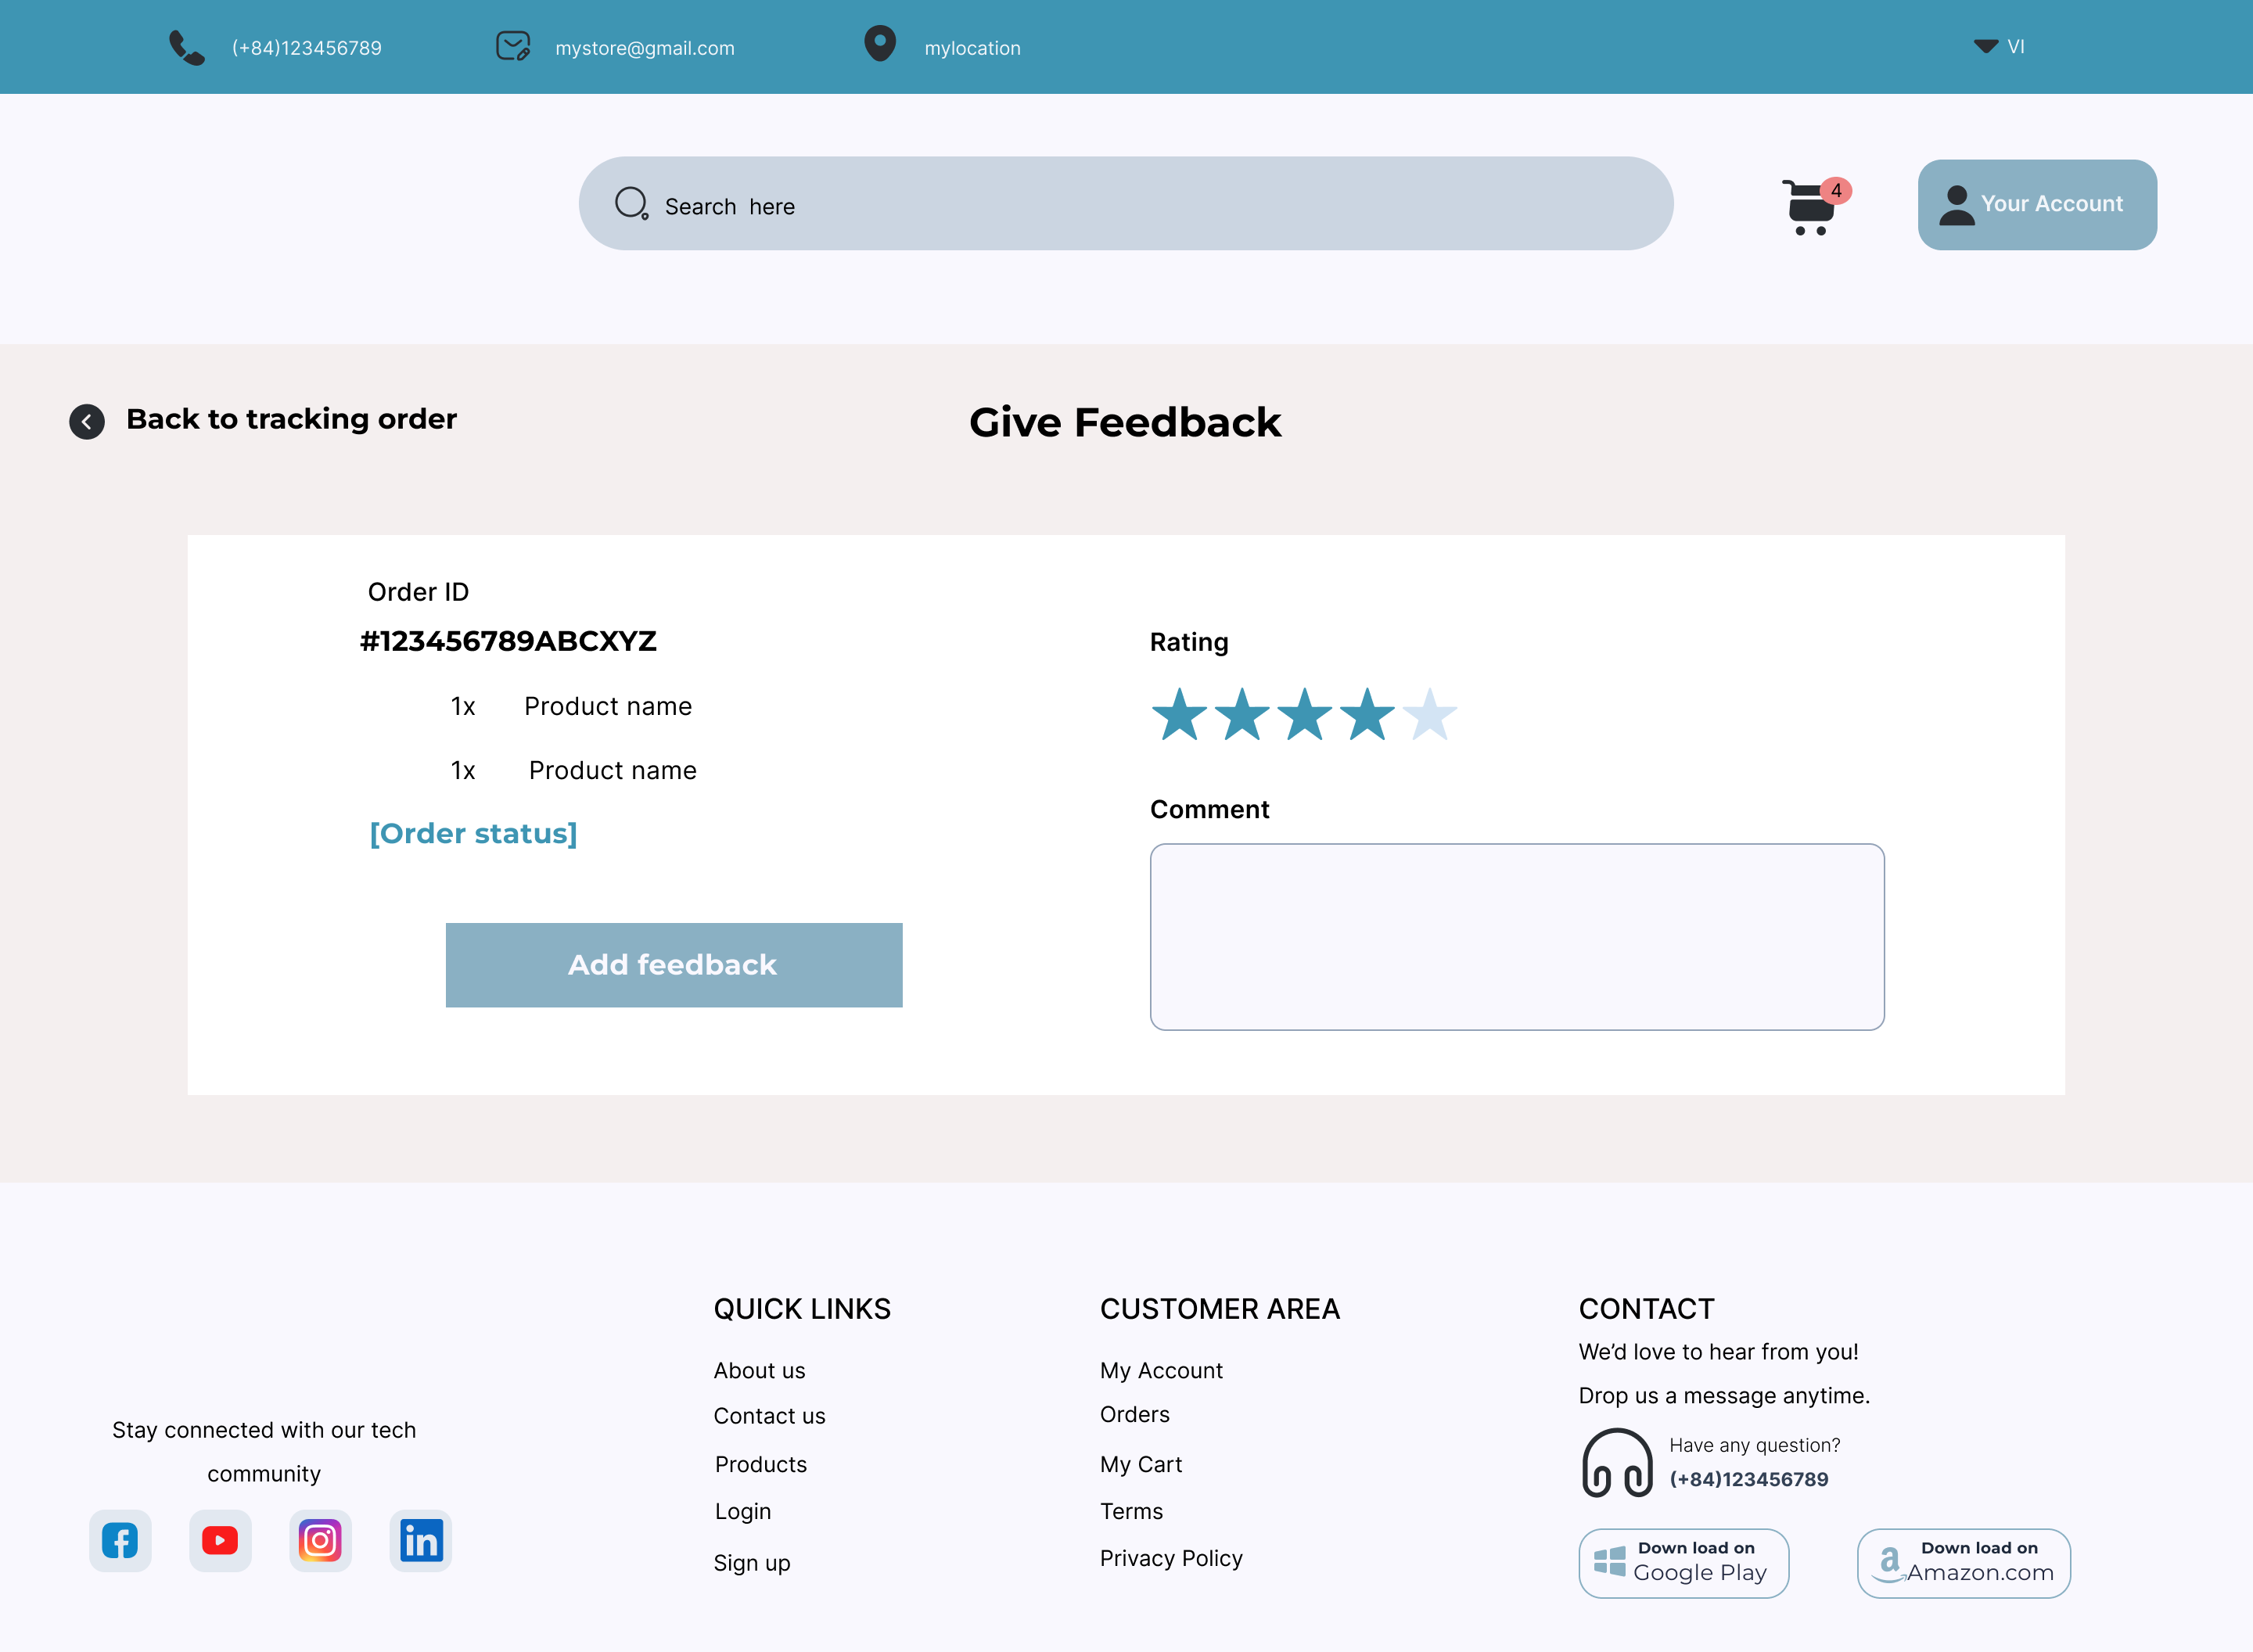
\includegraphics[width=0.8\linewidth]{images/ui/ui_give_feedback.png}
   \vspace{0.5cm} \caption{Giao diện Đánh giá sản phẩm}
    \label{fig:ui_feedback}
\end{figure}
Cho phép người dùng để lại sao (rating) và bình luận (review) sau khi mua hàng thành công, góp phần xây dựng hệ thống tín nhiệm cho sản phẩm.

\subsection{Giao diện quản trị (Admin-Site UI)}

\begin{figure}[H]
    \centering
    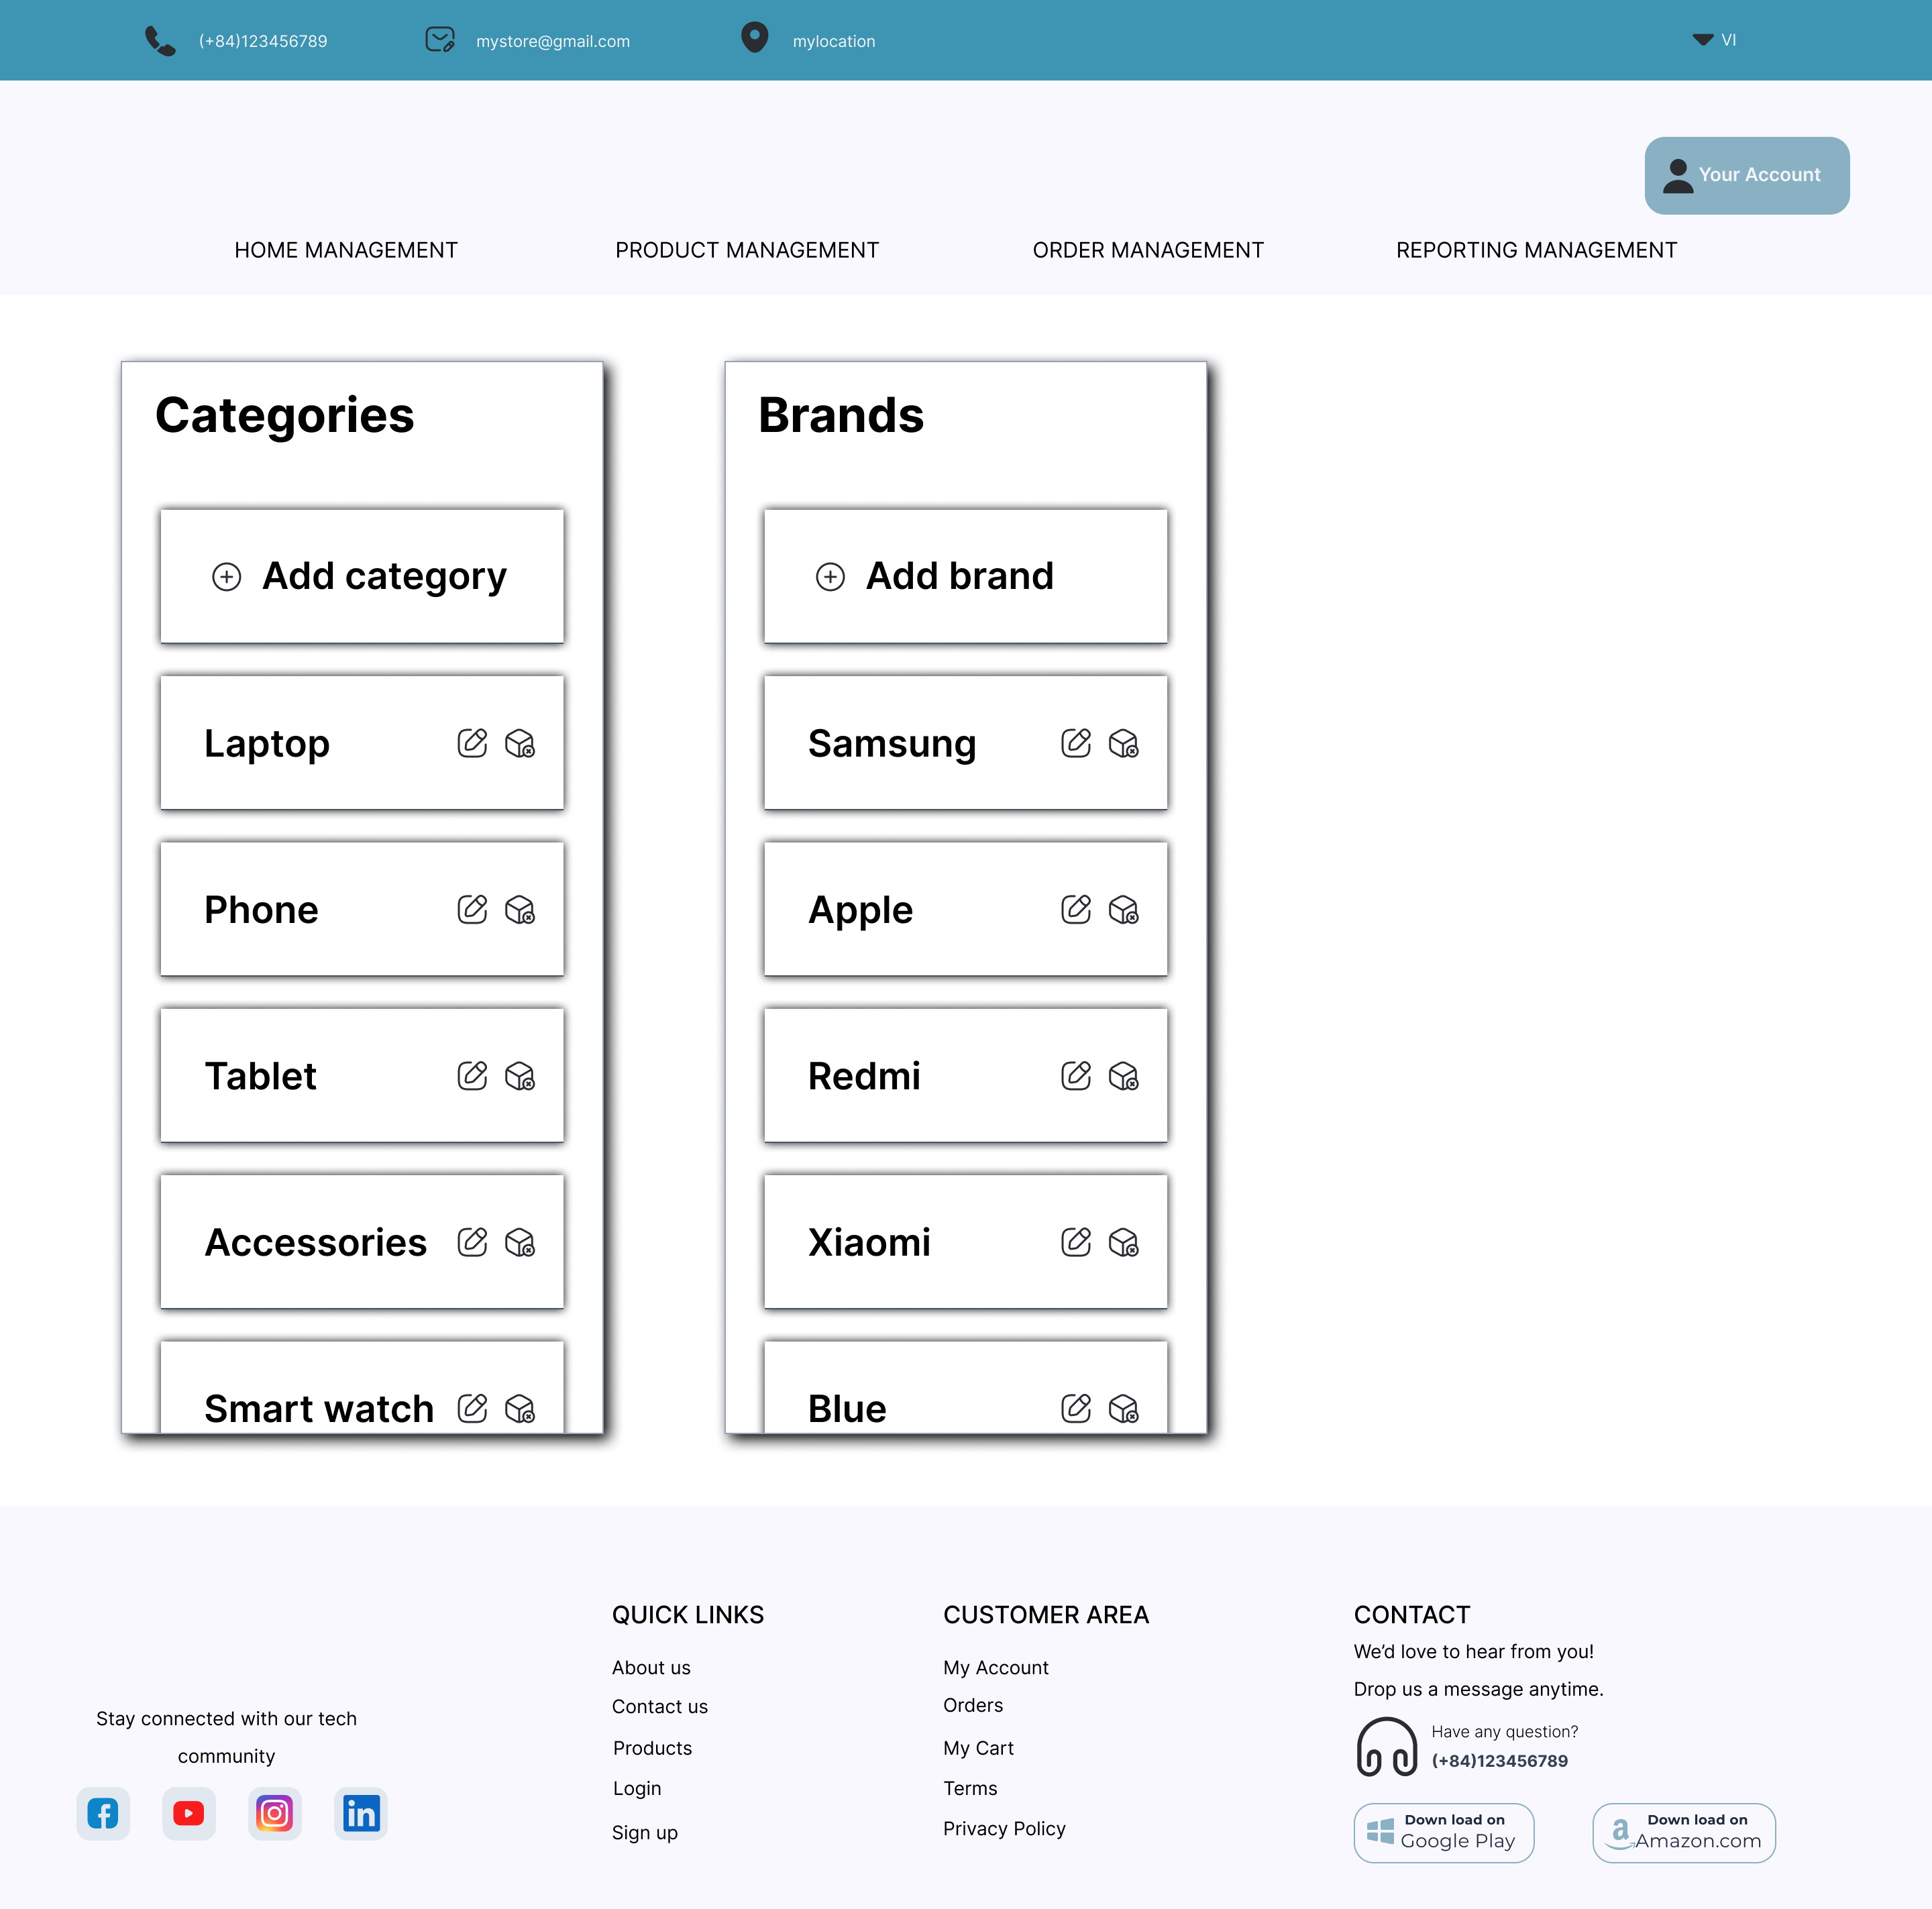
\includegraphics[width=1.0\linewidth]{images/ui/ui_admin_home.png}
   \vspace{0.5cm} \caption{Giao diện Dashboard quản trị (Admin Home)}
    \label{fig:ui_admin_home}
\end{figure}
Màn hình tổng quan dành cho quản trị viên, hiển thị các chỉ số kinh doanh quan trọng (KPIs) như: Doanh thu trong ngày, số lượng đơn mới, số lượng khách hàng mới đăng ký dưới dạng các thẻ (Cards) tóm tắt.

\begin{figure}[H]
    \centering
    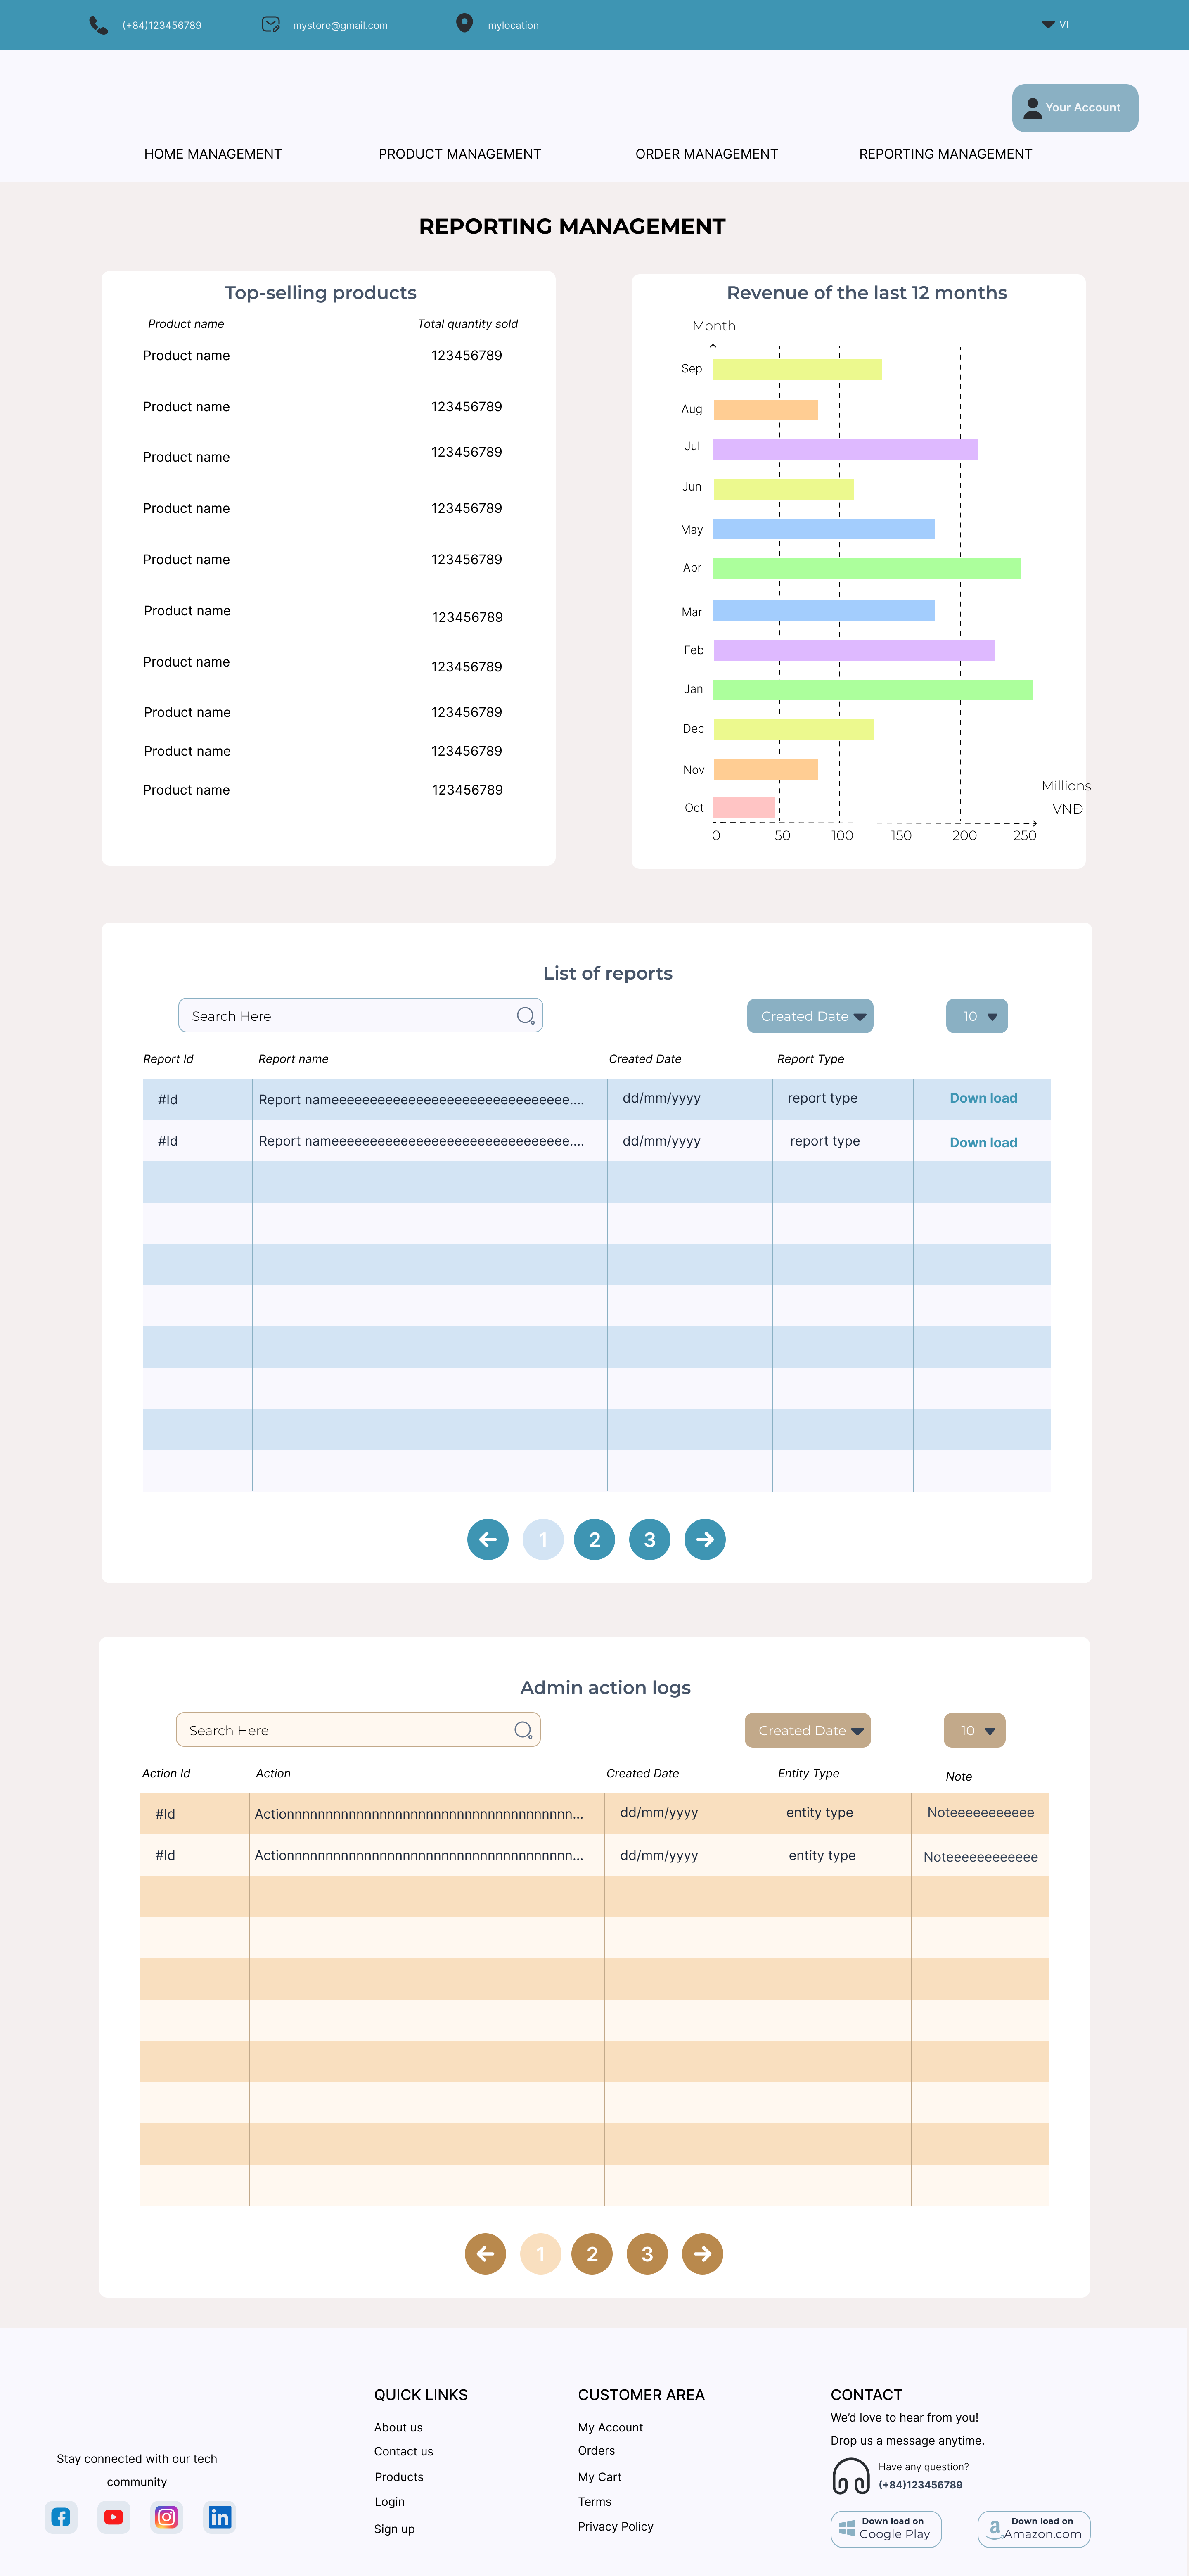
\includegraphics[width=0.6\linewidth]{images/ui/ui_report_management.png}
   \vspace{0.5cm} \caption{Giao diện Báo cáo thống kê}
    \label{fig:ui_admin_report}
\end{figure}
Cung cấp các biểu đồ trực quan (Biểu đồ cột, biểu đồ đường) để phân tích xu hướng doanh thu theo thời gian, sản phẩm bán chạy nhất và hiệu quả kinh doanh.

\begin{figure}[H]
    \centering
    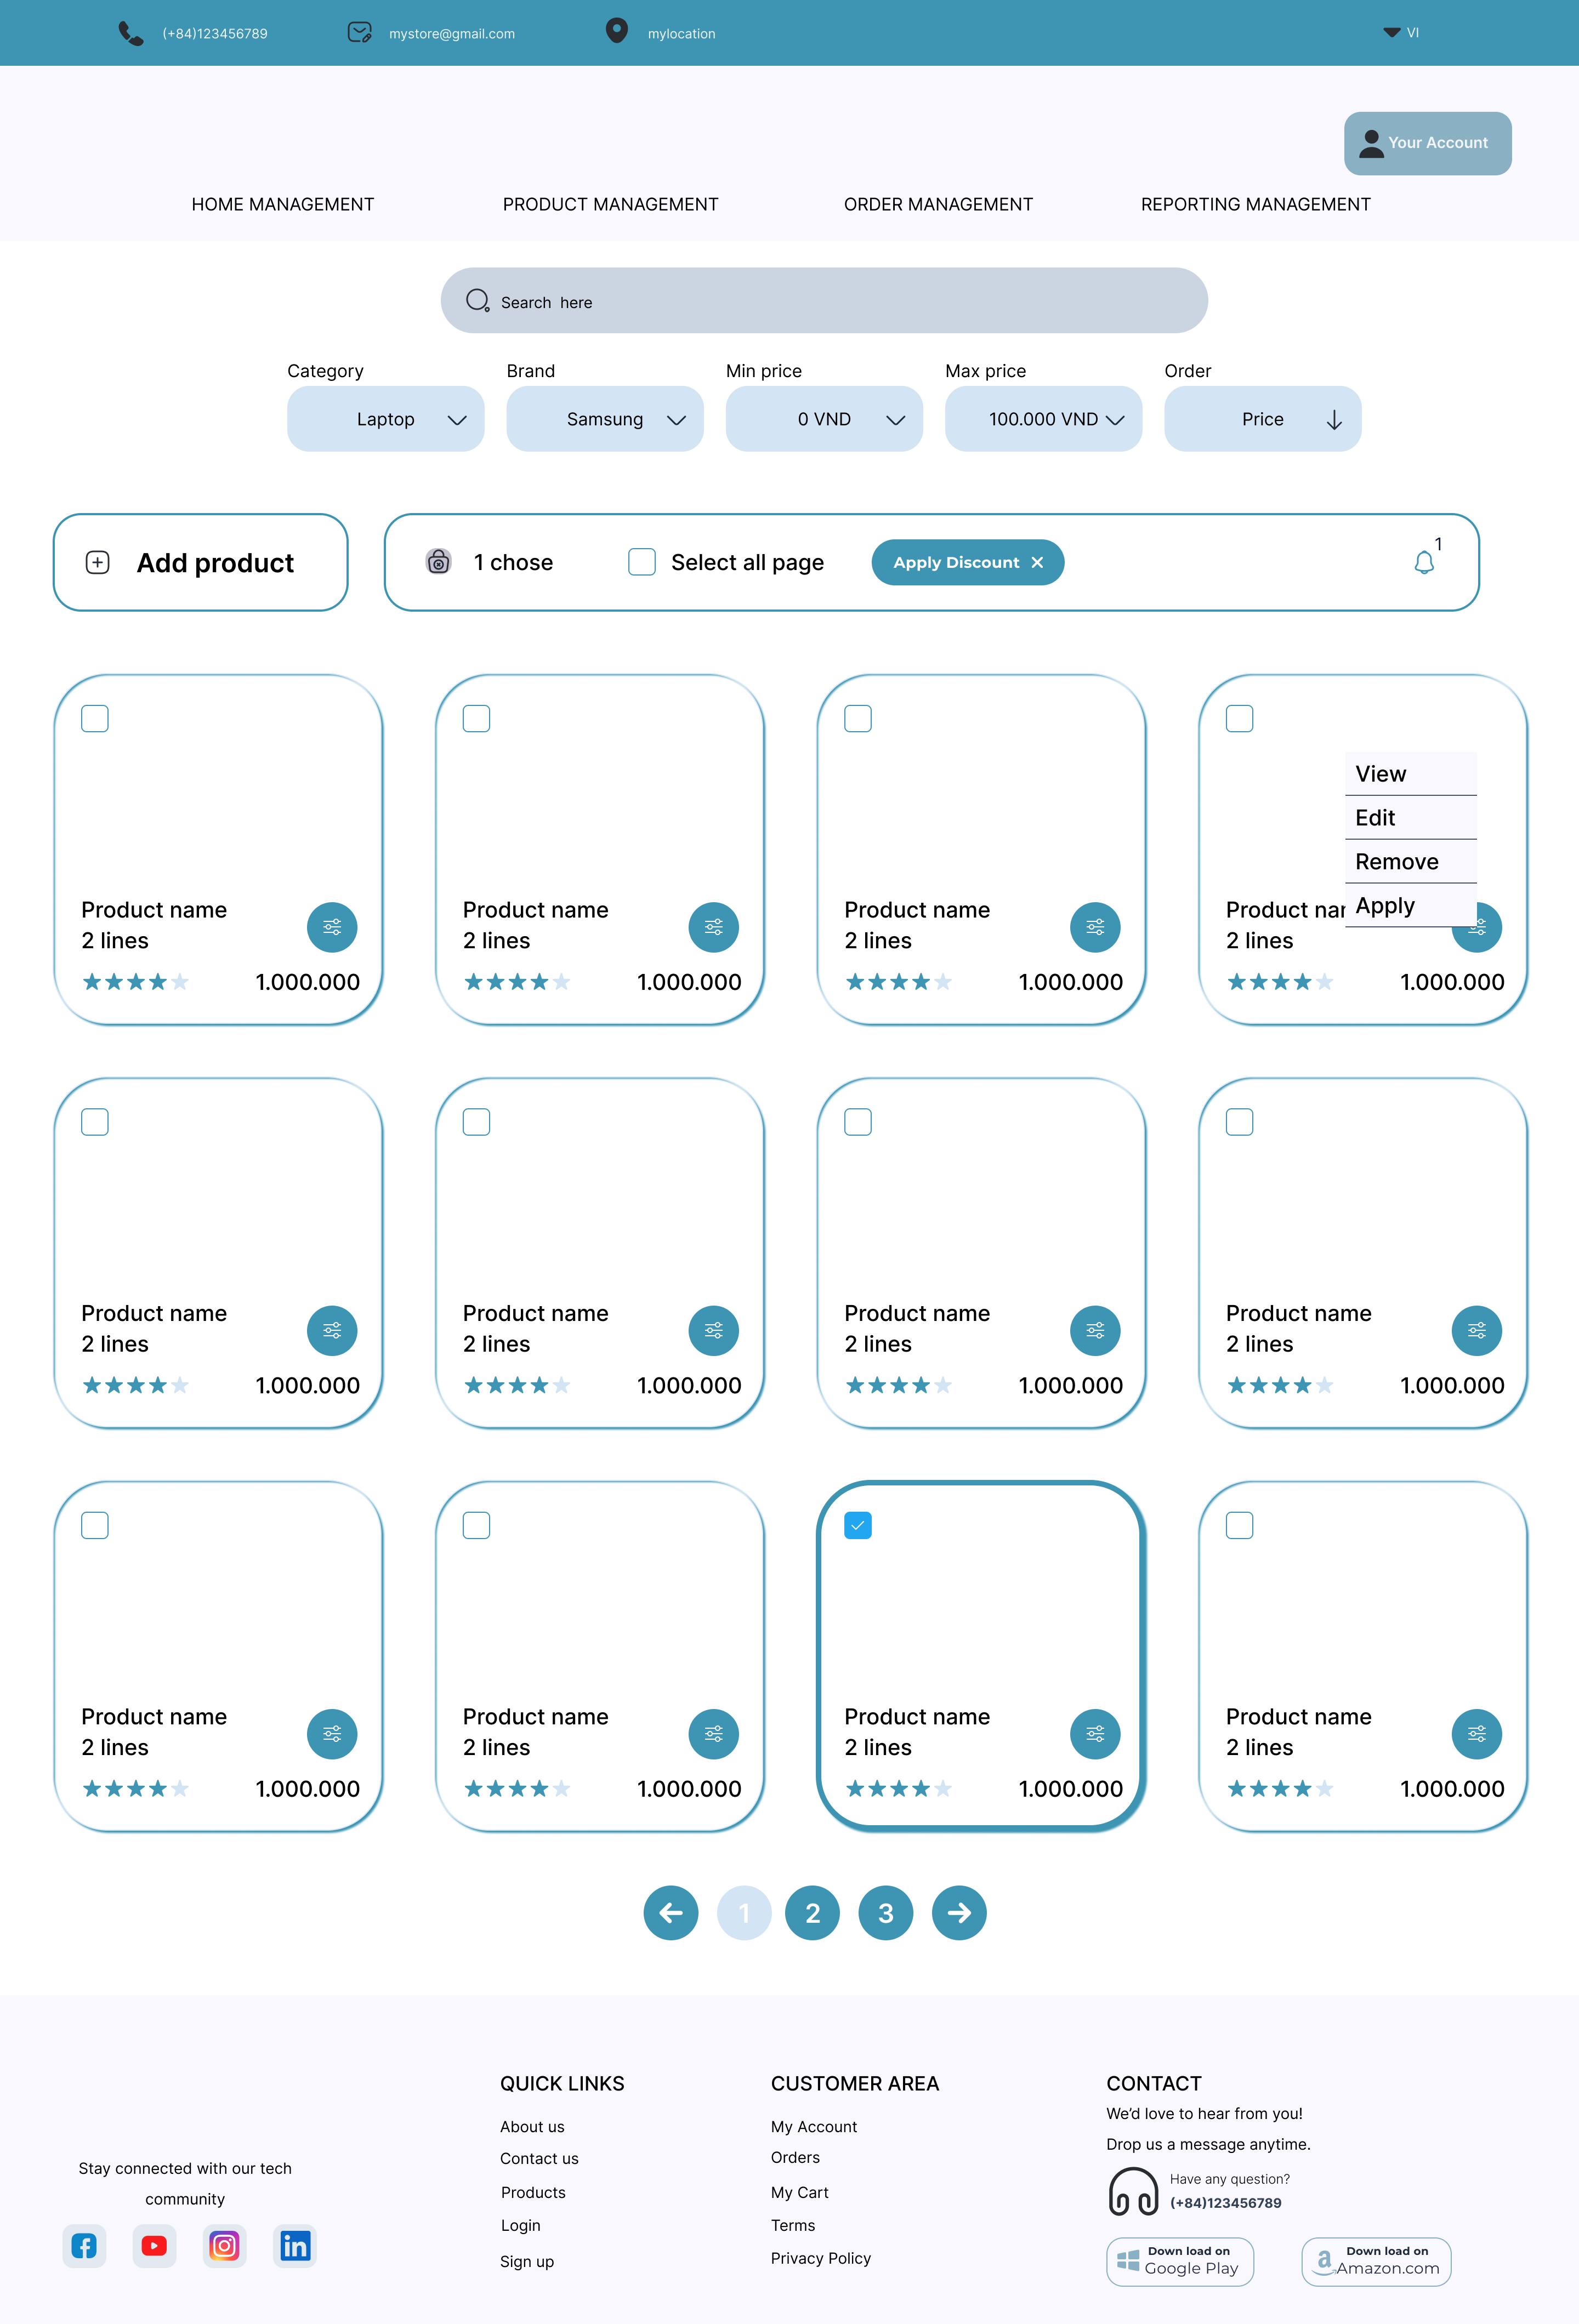
\includegraphics[width=1.0\linewidth]{images/ui/ui_admin_product.png}
   \vspace{0.5cm} \caption{Giao diện Quản lý sản phẩm (Admin)}
    \label{fig:ui_admin_product}
\end{figure}
Trang danh sách sản phẩm cho phép Admin thực hiện các thao tác CRUD (Thêm, Xem, Sửa, Xóa), quản lý tồn kho và cập nhật giá bán.

\begin{figure}[H]
    \centering
    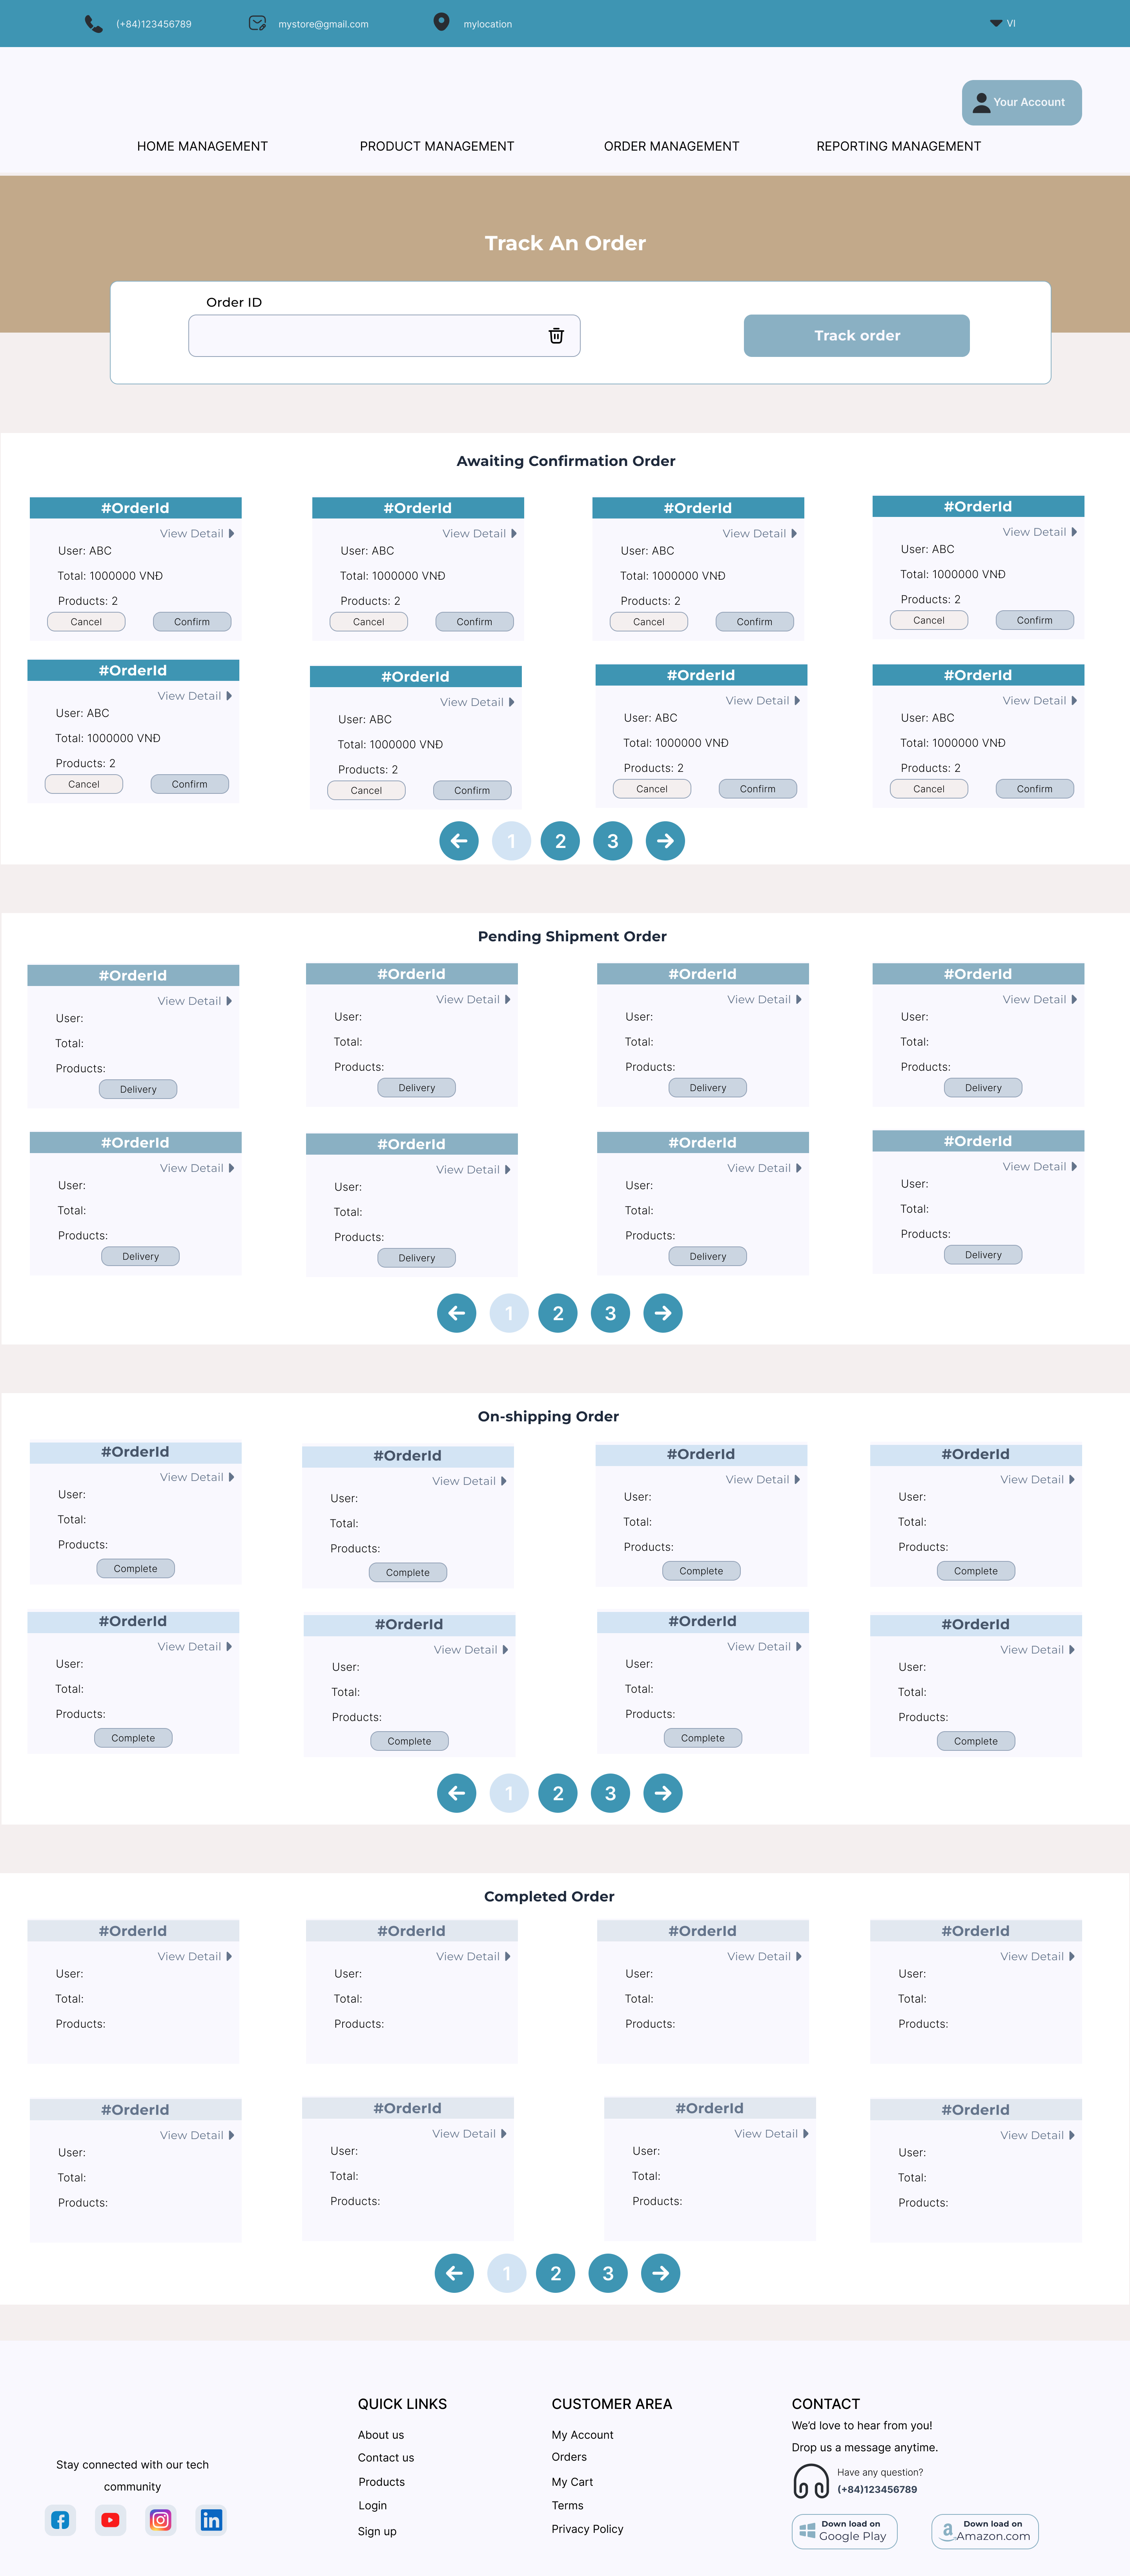
\includegraphics[width=0.6\linewidth]{images/ui/ui_order_management.png}
   \vspace{0.5cm} \caption{Giao diện Quản lý đơn hàng (Admin)}
    \label{fig:ui_admin_orders}
\end{figure}
Danh sách toàn bộ đơn hàng trên hệ thống, cho phép Admin lọc theo trạng thái để xử lý quy trình vận hành (Duyệt đơn, Đóng gói, Giao hàng).

\begin{figure}[H]
    \centering
    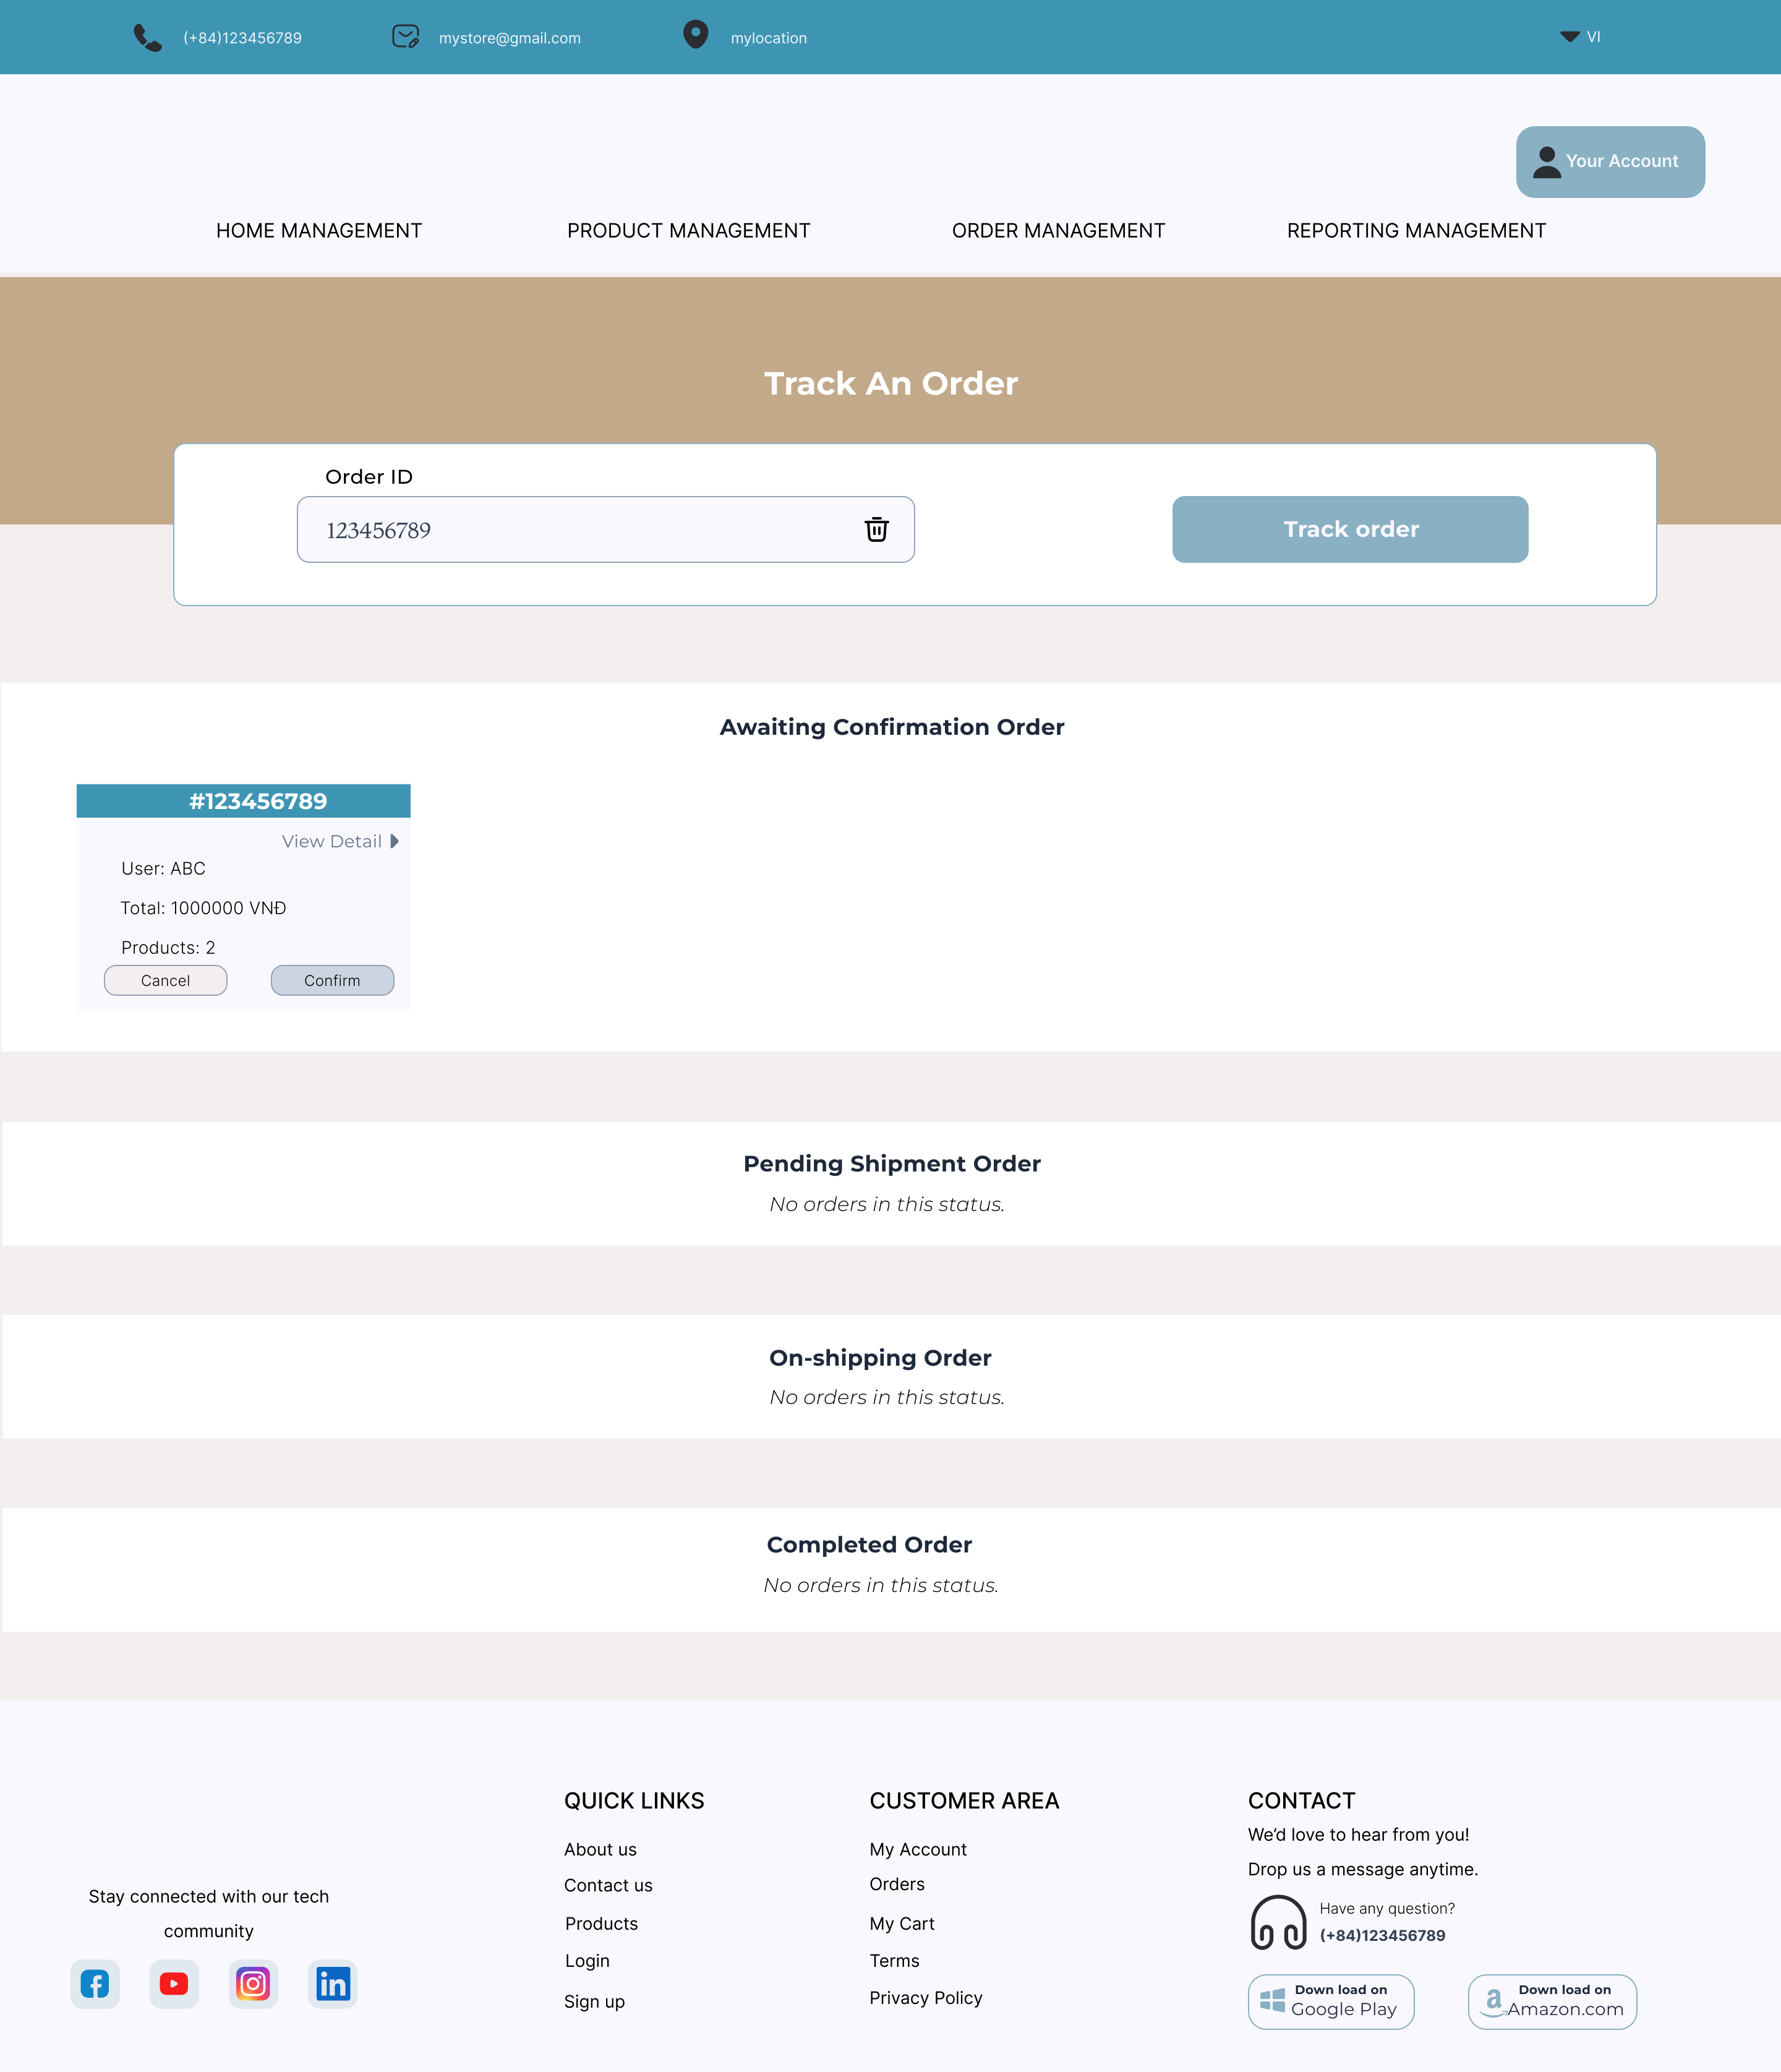
\includegraphics[width=1.0\linewidth]{images/ui/ui_order_management_track_one.png}
   \vspace{0.5cm} \caption{Giao diện Chi tiết xử lý đơn hàng}
    \label{fig:ui_admin_track_one}
\end{figure}
Giao diện chi tiết giúp Admin xem xét và cập nhật trạng thái thủ công cho từng bước của một đơn hàng cụ thể khi có sự cố phát sinh.